\documentclass[12pt]{article}
\usepackage{multirow}
\PassOptionsToPackage{a4paper,left=30mm,top=20mm,right=20mm,bottom=30mm}{geometry}
%\usepackage[backend=biber,style=numeric]{biblatex} % Use biblatex with numeric citations
\usepackage{cite}
\usepackage{hyperref}  
\usepackage{tikz}
\usetikzlibrary{positioning}
\usepackage{subcaption}
\usepackage{ulem} 
\usepackage{comment}
\usepackage{amsmath}
\usepackage{float} 
\setlength{\parskip}{0.5em}
% Enable clickable references
\usepackage{graphicx}        
\usepackage{array}
\usepackage[margin=0.8in]{geometry}
\usepackage{adjustbox}
\usepackage{makecell}
\usepackage{csvsimple}
\usepackage{amssymb}
\usepackage{setspace}

\onehalfspacing
\newcommand{\Sarp}[1]{{\textcolor{blue}{{SA: #1}} }}
\newcommand{\Sean}[1]{{\textcolor{red}{{Sean: #1}} }}
\newcommand{\todo}[1]{\textcolor{orange}{\texttt{TODO: #1}}}



\usepackage{cite} % For citation handling
\bibliographystyle{acm}  
 % without .bib extension

\title{FYP }
\author{Sean White}
\date{January 2025}

\begin{document}

\maketitle


\abstract{
\begin{itemize}
    \item Motivated by the need for fast and accurate models of gravitational waveforms, this project explores Gaussian Process Regression (GPR) as a way to model the waveform mismatch in black hole binary mergers.
    \item Begin by understanding GPR fundamentals on a low-dimensional toy problem following \cite{bible},.
    \item We extend this approach to a 4-dimensional and 7-dimensional parameter space, derived from the 8D intrinsic black hole parameter set.
    \item Multiple kernels (RBF, Matern, RationalQuadratic, Laplacian) and noise modelling techniques (homoscedastic, heteroscedastic) are compared.
    \item Using cross-validation and metrics \cite{metrics}, we find that several models are very accurate with the best models achieving .......
    \item We also apply MCMC to sample hyperparameter posteriors and understand how uncertain our predictions are. Emphasis maybe how MCMC is ideal but too computationally expensive 
    \item Visualise the GPR across its parameter space taking cross-cuts
    \item Finally our GPR provides a fast and accurate mismatch model that will help the work being carried out in \cite{Ogpaper}.
\end{itemize}
}


\section{Gravitational Waves Background}
\subsection{General Relativity intro}
\label{sec:GRintro}
Gravitational waves (GWs) are small fluctuations of spacetime that propagate at the speed of light. In the simplified linearized theory, we assume a flat Minkowski spacetime, and the small fluctuations around it are referred to as gravitational waves. The term ``waves'' is justified since, in an appropriate gauge (specific choices of coordinates), \(h_{\mu\nu}\) satisfies the wave equation. This is described in detail in Gravitational Waves, Vol. 1 by Maggiore~\cite[Sec~ 1.1]{GRbook}.
Formally we appproach this by expanding Einstein equations around the flat Minkowski metric $\eta _{a b}$ 
\begin{equation}
g_{ab} = \eta_{ab} + \epsilon\,h_{ab},
\qquad
\epsilon \ll 1,
\qquad
\eta_{ab} = \mathrm{diag}(-1, 1, 1, 1),
\end{equation}
where \(h_{ab}\) represents the perturbation. In the linearized regime of general relativity, the Einstein field equations simplify to
\begin{equation}
    \Box \bar{h}_{ab} = \frac{-16\pi G}{c^4} T_{ab}.
\end{equation}
However we are interested in this equation outside of the source (i.e $T_{ab} =0$) therefore we are left with 
\begin{equation}
    \Box \bar{h}_{ab} = 0, 
\end{equation}
with \(\Box\) the d’Alembertian operator in flat spacetime.
%

Although \(h_{ab}\) initially has 10 independent components (as a symmetric $4 \times 4$ tensor), 8 of these correspond to gauge freedom and constraints. After imposing the Lorentz and transverse-traceless (TT) gauge conditions, only two physical degrees of freedom remain: the plus (\(h_+\)) and cross (\(h_\times\)) polarizations~\cite[Sec.~1.2]{GRbook}.
This wave equation admits plane-wave solutions. For a wave propagating in the \(z\)-direction, the TT-gauge form of the perturbation is
\begin{equation}
h_{ab}^{(\mathrm{TT})} \;\propto\;
\begin{pmatrix}
0 & 0 & 0 & 0 \\
0 & h_+ & h_\times & 0 \\
0 & h_\times & -h_+ & 0 \\
0 & 0 & 0 & 0
\end{pmatrix}
e^{i(kz-\omega t)}.
\end{equation}

% One can visualize \(h_+\) and \(h_\times\) by studying how freely-falling test particles in
% the \(x\)--\(y\) plane move under each polarization: \(h_+\) distorts along \(x\) and \(y\)
% axes, whereas \(h_\times\) acts on diagonals at \(\pm45^\circ\). In realistic astrophysical
% sources, both polarizations are generally present.

\subsubsection*{Leading-Order Power Emission by Gravitational Waves}
\label{subsec:GW_power}

In general, the power emitted by a radiative field can be expressed schematically as
\begin{equation}
    \dot{E} = \sum_{\ell = 0}^{\infty} \left\langle \left| \left( \frac{\partial}{\partial t} \right)^{\ell+1} P_\ell(t) \right| \right\rangle.
\end{equation}
Here, \(P_{\ell}(t)\) represents the multipole moments of the radiating source. The \(\ell = 0\) term corresponds to the monopole moment, which in the gravitational case is the total mass of the system. Assuming mass is conserved, this term vanishes.
The \(\ell = 1\) term represents the dipole moment, which is also zero in the gravitational case due to conservation of linear momentum. Therefore, the leading-order contribution to gravitational-wave emission arises from the \(\ell = 2\) term, known as the quadrupole radiation.
This gives the leading-order expression for the power emitted in gravitational waves
%
\begin{equation}
\dot{E} = \frac{G}{5\,c^5}
\left\langle \dddot{Q}_{ij}\,\dddot{Q}^{\,ij} \right\rangle,
\end{equation}
%
where \(Q_{ij}\) is the mass quadrupole moment of the source. It is related to the mass moment \(M_{ij}\) by
%
\begin{equation}
Q_{ij} := M_{ij} - \frac{1}{3} \delta_{ij} M^k_{\ k},
\end{equation}
where \(M_{ij} = \int d^3x\, T^{00}x^i x^j\).



\subsubsection*{Quasi-circular Inspiral of two Point Masses}
\label{subsec:two_mass_example}
We will now consider a generic problem as illistrated in \cite{intoGRSarp} where two point masses, \(m_1 \ge m_2\), are in a quasi-circular orbit of separation \(R\),
each at distances \(r_1\) and \(r_2\) from their common center of mass (CoM), with
\(R = r_1 + r_2\). We place the orbit in the \(x\)--\(y\) plane so that mass~1 moves on
\(\mathbf{x}_1(t) = r_1(\cos\Omega t,\,\sin\Omega t)\) and mass~2 on
\(\mathbf{x}_2(t) = r_2(\cos(\Omega t+\pi),\,\sin(\Omega t+\pi))\). The system’s orbital
frequency is \(\Omega\). A short calculation yields
%
\begin{equation}
    Q^{ij} = 4 \Omega^3 \left(m_1 r_1^2 + m_2 r_2^2\right)
    \begin{pmatrix}
    \sin(2\Omega t) & -\cos(2\Omega t) \\
    -\cos(2\Omega t) & -\sin(2\Omega t)
    \end{pmatrix}.
\end{equation}
%
%
Introducing the reduced mass \(\mu = m_1 m_2/(m_1 + m_2)\), we get that the \(\ell=2\) power emission is
%
\begin{equation}\label{eq:E_dot_2}
\dot{E}_{\ell=2}
\;=\;
\frac{32}{5}\;\frac{G}{c^5}\;\Omega^6\,\mu^2\,R^4.
\end{equation}
Both \(\Omega\) and \(R\) are functions of time, but they evolve on a time scale (radiation reaction) much longer than the orbital time
scale and so when averaging over orbits we approximate them as constant. Applying Kepler’s law, \(\Omega^2 = GM/R^3\), and defining
\(\omega = 2\Omega\) as the GW frequency, we find
%
%
\begin{equation}
\dot{E}_{\ell=2}
\;=\;
\frac{32}{5}\;\frac{c^5}{G}
\left(\frac{G\,\mathcal{M}\;\omega}{2c^3}\right)^{10/3},
\quad
\text{where}
\quad
\mathcal{M} \;=\;\mu^{3/5}\,M^{2/5}
\label{eq:Energy}
\end{equation}
%
is known as the chirp mass where $M = m_1+m_2$ is the total mass.
%
%
$ \dot{E} $ represents the rate at which the system loses energy due to gravitational-wave emission.
This energy loss causes the binary orbit to shrink and the GW frequency to increase, 
with the chirp mass \(\mathcal{M}\) and frequency \(\omega\) capturing the key features of this inspiral.

% Quick comment about frequency extra I think
% Using conservation of energy and the \eqref{eq:Energy}, we find the gravitational-wave frequency evolves as:
% \begin{equation}
% \dot{f} \propto f^{11/3},
% \end{equation}
% highlighting that the GW frequency grows as the system radiates.
In general, an incoming GW manifests itself as a time series of GW strain given by
%
\begin{equation}
 h(t) = h_+(t) - i h_\times(t), \label{eq:GW_strain}
\end{equation}
%
where $ h_+, h_\times$ are the two physical degrees of the GW known as the polarizations.
For the case of the simple quasi-circular inspiral introduced above, 
the polarizations can be expressed in terms of the characteristic strain \( h_c(t) \) [see \cite[Sec.~4.1]{GRbook}]] 
which captures the amplitude of the waveform
\begin{subequations}
\begin{align}
h_+(t) &= h_c(t) \left( \frac{1 + \cos^2\iota}{2} \right) \cos[\Phi_N(t)],
\label{eq:hp_time}\\
h_\times(t) &= h_c(t) \cos\iota \sin[\Phi_N(t)],
\label{eq:hc_time}\\
h_c(t) &= \frac{4}{D} \left( \frac{G \mathcal{M}}{c^2} \right)^{5/3} \left( \pi f(t) \right)^{2/3}
\label{eq:char_strain}.
\end{align}
\end{subequations}
Here \(\iota = \cos^{-1}(\hat{n} \cdot \hat{L}) \) is the inclination angle between the line-of-sight unit vector \( \hat{n} \) and the orbital angular momentum unit vector \( \hat{L} \),
\( \mathcal{M} \) is the chirp mass, and
\( D \) is the distance to the source.
As the frequency \( f(t) \) increases, so too does \( h_c(t) \), giving rise to the characteristic chirping waveform.

\Sean{Confused on frequency domain, It is a fourier transform of this??? Maybe plot of chirping behaviour}
\Sarp{Yes, it is the Fourier transform using SPA. I'll show you where to find the relevant expressions.
See Maggiore Eqs.(4.34, 4.35)}


\subsubsection*{Introducing the Waveform Mismatch}
\label{subsec:mismatch_intro}
%
%
This simplified two-mass, circular-orbit model captures the main physical features of an inspiraling binary system such as the characteristic chirp behaviour. However, it omits several key physical effects such as orbital eccentricity and the spin of each mass. 
To quantify how these simplifications affect the accuracy of the waveform, we would compute the mismatch of
the simpler waveform, $h_\text{simple}$, to more faithful (accurate) waveforms. 
\Sarp{Maybe use $h_i$ for simple WF and $h_0$ for the faithful waveform?}
%
%
The mismatch between two signals is defined by \cite{mismatch, Ogpaper}
\begin{equation}
\label{eq:mismatch_def}
\mathcal{M} 
\;=\; 
1 \;-\;
\max_{\mathbf{\lambda_m}}
\frac{\langle h_{\text{simple}},\,h_{\text{accurate}}\rangle}
{\sqrt{\langle h_{\text{simple}},h_{\text{simple}}\rangle \,
\langle h_{\text{accurate}},h_{\text{accurate}}\rangle}},
\end{equation}
where \(\langle\cdot,\cdot\rangle\) is the inner product of both GW, 
\Sarp{You need to provide the equation for the inner product as well, it is an integral in the frequency domain that
is weighted by the detector's amplitude spectral density (sensitivity)}
and we maximise over a set of (intrinsic and/or extrinsic) model parameters \(\mathbf{\lambda_m}\) depending on the type of mismatch we wish to compute.
\Sarp{Maybe refer to the section where you introduce the parameters}
A mismatch \(\mathcal{M}\ll 1\) indicates that our simple waveform
faithfully represents the physical signal, whereas larger mismatches highlight missing
physics ( overly simplified).




\subsection{GW Approximation using Bayesian Methods}
\label{sec:GW_and_Bayes}

In Section~\ref{sec:GRintro} we focused on linearised theory and a simple Newtonian two-body inspiral model. This helped motivate the ideas behind gravitational wave generation and emisson.
However the gold standard for generating gravitational waveforms is to directly solve the full Einstein equations via numerical relativity (NR),
but, the computational cost is enormous, and therefore only a limited number of NR simulations are currently available.
Consequently, many analytic or semi-analytic GW models have been created that are calibrated to these NR simulations.
As each waveform model makes a various set of differing assumptions to others models, it introduces model-specific
errors and potentially biases.
We utilise the mismatch between signals discussed in Section~\ref{subsec:mismatch_intro} 
to quantify how faithful GW waveforms generated by a given model are to the NR simulations.

The standard approach to account for modelling errors when inferring the properties of binary black holes is to construct a mixture model, where results from numerous waveform models are combined.
Bayesian methods have been utilised here to build posterior distributions for each model over intrinsic model parameters (Mass, Spin vectors) given the data. Different approaches exist for combining these posteriors:
\begin{itemize}
    \item Standard Method: Combine all model-specific posterior distributions with equal weights, yielding a single mixture distribution that, in practice, may ignore large differences in model fidelity (\cite{linearcombination}).
    \item Evidence-Informed Method \cite{Bayesianapproach}: Weigh each model by its Bayesian evidence i.e., by how well it fits the observed data overall. This approach is commonly referred to in the gravitational-wave literature. 
\end{itemize}

Recent work by Hoy, Akcay and collaborators~\cite{Ogpaper} emphasized that some waveform models may be more faithful to full NR solutions in certain regions of parameter space (e.g., certain mass ratios or spin orientations),
while others do better in other regions. An evidence-based method that uses an overall Bayes factor does not account for local differences if, for example, one waveform is slightly worse globally but significantly better locally.
To address this limitation, Hoy et al.\cite{Ogpaper} introduced an approach which prioritizes whichever model is locally more accurate, thereby mitigating bias.
They showed that this new technique can use up to 30\% fewer computational resources while recovering the true parameters more faithfully compared to standard mixture methods.
This numerical relativity informed method used model mismatch to inform how accurate models were in certain parameter spaces and then using Bayesian methods choice models with better 
mismatch scores in different parameter spaces.


\subsection{Project Motivation}
Although the NR-informed method is conceptually appealing, it requires us to know (or at least to estimate) 
the mismatch of each model throughout the parameter space of interest. Because
NR simulations are costly, we cannot generate an exhaustive library of NR waveforms
everywhere. This is where the work summarized in this report contributes.

We propose to build a GPR model that interpolates the mismatch as a function of parameters. Specifically, from a finite set of computed mismatches (obtained at a limited but carefully chosen set of parameter points), we train a GPR. The trained model can then predict the mismatch in the untested regions of parameter space. This approach circumvents the need for high-resolution NR simulations at every point of interest,
offering an efficient and scalable alternative. The Gaussian Process framework is advantageous because it not only provides a smooth interpolation but also yields uncertainty estimates for its predictions.
 As more NR data become available, the GPR can be updated or retrained, systematically improving the global mismatch predictions.

 In summary, by modeling the mismatch between approximate waveforms and NR waveforms via GPR, we can better implement the mismatch-driven approach introduced by Hoy et al.~\cite{Ogpaper}. This strategy reduces bias from using just a single “global best” model and leverages a sparse but valuable set of NR simulations to yield more accurate gravitational-wave parameter estimation.
\begin{comment}
\newpage
A motivating example for this is outlined below.
\begin{figure}[h] 
    \centering
\includegraphics[width=1.1\textwidth]{Images/image.png} % 120% of text width
    %\caption{}
    %\label{fig:example-image}
\end{figure}

the black contours here represent a ratio of the mismatch between two different models for Gravitational Waveforms. Models used: model1: IMRPHENOMXPHM, model2: SEOBNRV5PHM, model3: IMRPHENOMTPHM. The left graph contours give the $\frac{mismatch(model1)}{mismatch(model2)}$ and right gives $\frac{mismatch(model3)}{mismatch(model2)}$. A mismatch ratio greater than 1 indicates that model 2 is closer to the NR simulations.
\end{comment}

\subsection{Data Description}
\label{sec:data_description}
We have discussed what the mismatch between wave signals is and why we want to model the mismatch between GW's from NR and GW's from analytical models.
Our proposed GPR method will take as inputs the intrinsic parameters of the binary black hole and will output the mismatch predictions.
The inrinsic parameter space of a binary black hole is 8 dimensional visualised in Figure~\ref{fig:gr_diagram}. This accounts for two masses and two spin vectors both in 3 dimensions. 
To generate this mismatch data we calculated the mismatch between waveform model \textsc{SEOBNRv5PHM}\todo{cite} and the NR surrogate \textsc{NRSur7dq4}\todo{cite} using eqn~\eqref{eq:mismatch_def} for a set of 250 intrinsic parameters 
such that it covers 5 different mass ratios and a grid of concentric ellipses in the spin projection space.
This 250 element set is then repeated for 4 different masses.
Each mismatch is further an average of 294 mismatches computed over a grid of 3 different extrinsic parameters.
See Hoy et al. for further details.
%

We reduce our eight-dimensional parameter space (two masses \(M_1\) and \(M_2\), and two spin vectors in three dimensions \(\mathbf{S} = (S_x, S_y, S_z)\)) to four parameters:
\begin{align}
    \begin{aligned}
    M_{\mathrm{tot}} & = M_1 + M_2, \\
    \eta & = \frac{q}{(1 + q)^2},
    \end{aligned}
    \hspace{1.5cm}
    \begin{aligned}
    \chi_{\parallel} &= \frac{\left|\mathbf{S}_{1,\parallel} + \mathbf{S}_{2,\parallel}\right|}{M_{\mathrm{tot}}^2}, \\
    \chi_{\perp} &= \frac{\left|\mathbf{S}_{1,\perp} + \mathbf{S}_{2,\perp}\right|}{M_{\mathrm{tot}}^2}.
    \end{aligned}
\end{align}
Here, \( q = \frac{M_2}{M_1} \) is the mass ratio, and \( \eta \) is the symmetric mass ratio. The parameters \( \chi_{\parallel} \) and \( \chi_{\perp} \) correspond to the magnitudes of the combined spin vectors projected parallel and perpendicular to the orbital angular momentum, respectively.
\begin{figure}[H]
    \centering
    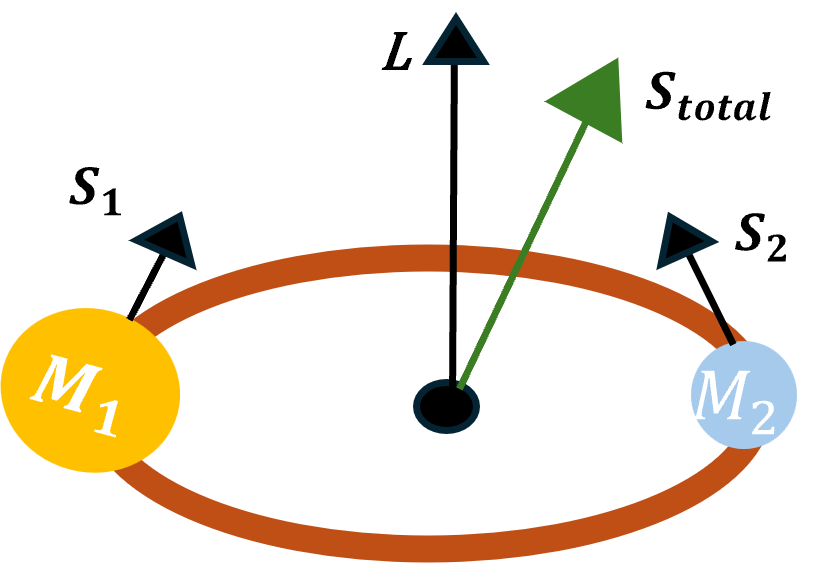
\includegraphics[width=0.4\textwidth]{LatexPlots/GRdiagram.png}
    \caption{GR diagram \todo{Write a better caption!}}
    \label{fig:gr_diagram}
\end{figure}
To assist in training our GPR model, we begin by scaling the input parameters. The total mass is scaled to lie in the interval \([0, 1]\), with four discrete values. For each total mass, the five values for the symmetric mass ratio are scaled to span the interval \([-1, 1]\). 
We also transform the spin data \((X_{\parallel}, X_{\perp})\) onto a uniform grid of size \(10 \times 25\), with:
\[
x \in \{0.1, 0.2, \ldots, 1\}, \qquad y \in \left\{-\frac{\pi}{2},-\frac{\pi}{2}+\frac{\pi}{24},\ldots, \frac{\pi}{2}\right\}.
\]
\begin{equation}
(x, y, z, w) = \text{transformed}(X_{\perp}, X_{\parallel}, \eta, M_{\text{tot}}),
\end{equation}
where \(x\), \(y\), \(z\), and \(w\) are the scaled inputs used in our GPR framework.

\begin{figure}[H]
    \centering
    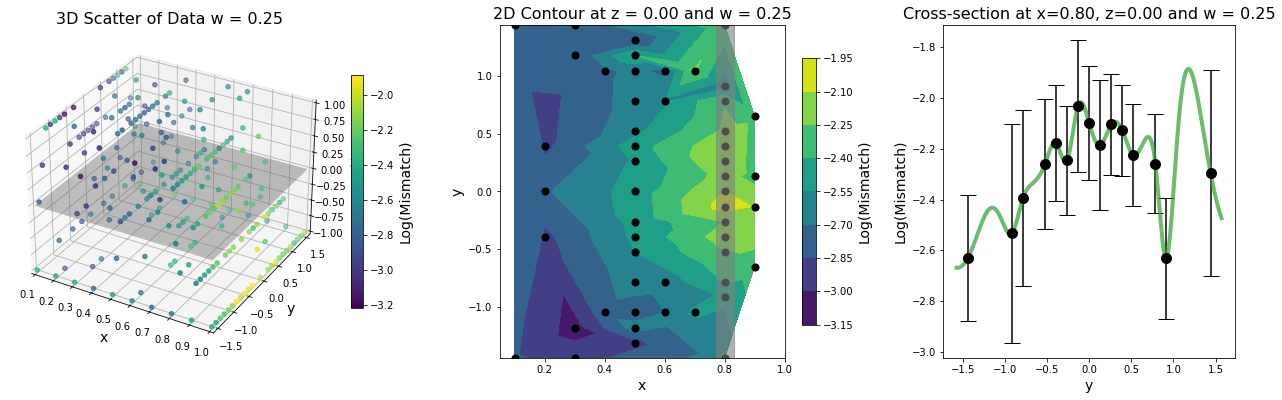
\includegraphics[width=1\textwidth]{LatexPlots/final_gps_plots/data_visual.png}
    \caption{
    Visualisation of the input data across reduced dimensions. 
    Left: A 3D scatter plot of all data points for fixed total mass \(w = 0.25\) ($M_\text{tot}=37.5 M_\odot$). 
    Centre: A 2D slice of the data at rescaled symmetric mass ratio \(z = 0\) ($q=0.404$), interpolated over spin components.
    Right: A 1D cut through the data at \(x = 0.8\) showing variation across \(y\). 
    When using raw data, interpolation is needed between samples, but GPR provides an analytic model that can be directly evaluated without interpolation.
    }
    \label{fig:visualising_data}
\end{figure}








\section{Gaussian Process Regression \textbf{GPR} Background}
\subsection{Introduction and Roadmap}

In the following subsections, I discuss the foundational concepts of Gaussian Process Regression \textbf{(GPR)} in four main steps:
\begin{enumerate}
    \item \textbf{Gaussian Processes Regression Background:} Section~\ref{sec: GP_backgroound} introduces Gaussian Processes and explains how their priors and posteriors are constructed from finite sets of points.
    \item \textbf{Kernel Functions:} In Section~\ref{sec: Kernels}, I explore how kernels encode the basic assumptions about smoothness and structural properties of the underlying function. I look at how kernel hyper-parameters effect the shape of samples from our prior distribution.
    \item \textbf{Noise Modeling:} Section~\ref{sec: Handlingnoise} covers several approaches for incorporating observational noise into the GP framework. I look at how noise effects the samples from our prior distribution.
    \item \textbf{Hyperparameter Optimization:} Finally, in Section~\ref{sec: Hyper_parameters}, I discuss how kernel and noise hyper-parameters can be optimised resulting in a posterior distribution that better explains our data.
\end{enumerate}

\subsection{Gaussian Proces Regression Background}
\label{sec: GP_backgroound}

\subsubsection*{Definition of a Gaussian Process}
\label{sec: Definition_of_GP}

A Gaussian Process \textbf{(GP)} defines a probabilistic model over all possible functions rather than assuming a single function to be true
\begin{equation}
f(X) \sim \mathcal{GP} (\mu(X), k(X, X')).
\label{eq: Initial_GP_distribution}
\end{equation}

\noindent
where \( \mu(X) \) is the mean function, specifying the expected function value at each \( X \):
\begin{equation}
    \mu(X) = {E}[f(X)],
    \label{eq: meandef}
\end{equation}

\noindent
 \( k(X, X') \) is the covariance function (kernel), encoding the relationships between function values at different points:
\begin{equation}
    k(X, X') = \text{Cov}(f(X), f(X')).
    \label{eq: kerneldef}
\end{equation}

\noindent
Since the input space is continuous, the GP represents an infinite-dimensional distribution. 
In practice, we approximate the process by evaluating the GP at a finite set of inputs.
These function values are then assumed to follow a multivariate normal Gaussian distribution.

\noindent
Mathematically, for a finite set of input points

\begin{equation}
X = \{X_1, X_2, \dots, X_n\},
\end{equation}
 the corresponding function values
\begin{equation}
f = \{f(X_1),f(X_2),...,f(X_n), \}
\end{equation}
follow a multivariate normal distribution
\begin{equation}
f \sim \mathcal{N}\left(\mu(X), K(X, X)\right).
\label{eq: Multivariate_distribution}
\end{equation}

\noindent
Each sample from this multivariate distribution represents a function evaluated at \( n \) different points.

\subsubsection*{The Prior Distribution}
\label{sec: prior_dist}

Before observing any data, we assume a joint Gaussian distribution over both training and test points. Let \( X \) denote training inputs and \( X_* \) test inputs. 
The joint prior over their function values is
\begin{equation}
\begin{bmatrix}
f(X) \\
f(X_*)
\end{bmatrix}
\sim \mathcal{N}
\left(
\begin{bmatrix}
\mu(X) \\
\mu(X_*)
\end{bmatrix},
\underbrace{
\begin{bmatrix}
K(X, X) & K(X, X_*) \\
K(X_*, X) & K(X_*, X_*)
\end{bmatrix}
}_{\mathcal{C} = \text{Covariance Matrix}}
\right).
\label{eq: Multivariate prior}
\end{equation}

\noindent
The corresponding joint probability density function (pdf) is given by:

\begin{equation}
    p(f, f_*) = \frac{1}{(2\pi)^{n/2} \sqrt{|\mathbf{C}|}} \exp\left( 
    - \frac{1}{2}\left(\begin{bmatrix}f \\f_*\end{bmatrix}-
    \begin{bmatrix}\mu(X) \\\mu(X_*)\end{bmatrix}\right)^T
    \mathbf{C}^{-1}\left(
    \begin{bmatrix}f \\f_*\end{bmatrix}-
    \begin{bmatrix}\mu(X) \\\mu(X_*)\end{bmatrix}\right)\right)
\end{equation}
    

\noindent
After accounting for the mean, the resulting distribution is entirely determined by its kernel function.
The kernel governs how the model generalizes to unseen data. There are many kernel choices, each encoding different structural assumptions about the function, such as smoothness, periodicity, or linearity.
In the next section we examine the different kernel choices available and the assumptions that each kernel encodes about our function structure, such as smoothness and periodicity.



\subsection{Kernel Functions}
\label{sec: Kernels}
The kernel function encodes our assumptions about the relationship between input points in a Gaussian Process (GP).
It defines the covariance between any two function values and thereby determines the smoothness, periodicity, or other properties of the functions drawn from the GP prior.
Fundamentally, kernels reflect the idea of similarity: input points \( x \) and \( x' \) that are close together are assumed to have highly correlated outputs \( f(x) \) and \( f(x') \),
while distant inputs are assumed to produce less correlated values. This notion of similarity, as emphasized in \cite[p.~79]{bible}, is central to how Gaussian processes learn from and generalize beyond training data.

\vspace{1em}
\noindent
In Figure~\ref{fig: samples_from_GP_prior}, we illustrate the effect of the kernel on the GP prior.
We draw three functions from the multivariate Gaussian prior defined in Equation~\ref{eq: Multivariate prior}, using a zero mean and an RBF kernel.
The first subplot shows these samples, while the second subplot visualizes the corresponding covariance matrix as a heatmap.
The matrix reveals that correlations are strongest when input points are close together (near the diagonal) and decay as the distance between inputs increases.
This is evident also from the samples as we can see nearby points often move in similar directions, while distant points diverge more significantly.

\vspace{1em}
\noindent
The final three subplots highlight how this distance-based correlation manifests in the joint distribution of pairs of function values.
For closely spaced inputs, such as \( (x, x') = (0, 0.1) \), the joint distribution of \( (f(0), f(0.1)) \) forms a narrow elliptical contour,
indicating strong correlation (approximately 0.9). As the distance increases, such as in the pairs \( (0, 0.5) \) and \( (0, 1) \), the ellipses widen, reflecting weaker correlation. This visualization reinforces the intuition that kernel functions govern how input proximity translates to output similarity.

\begin{figure}[H]
    \centering
       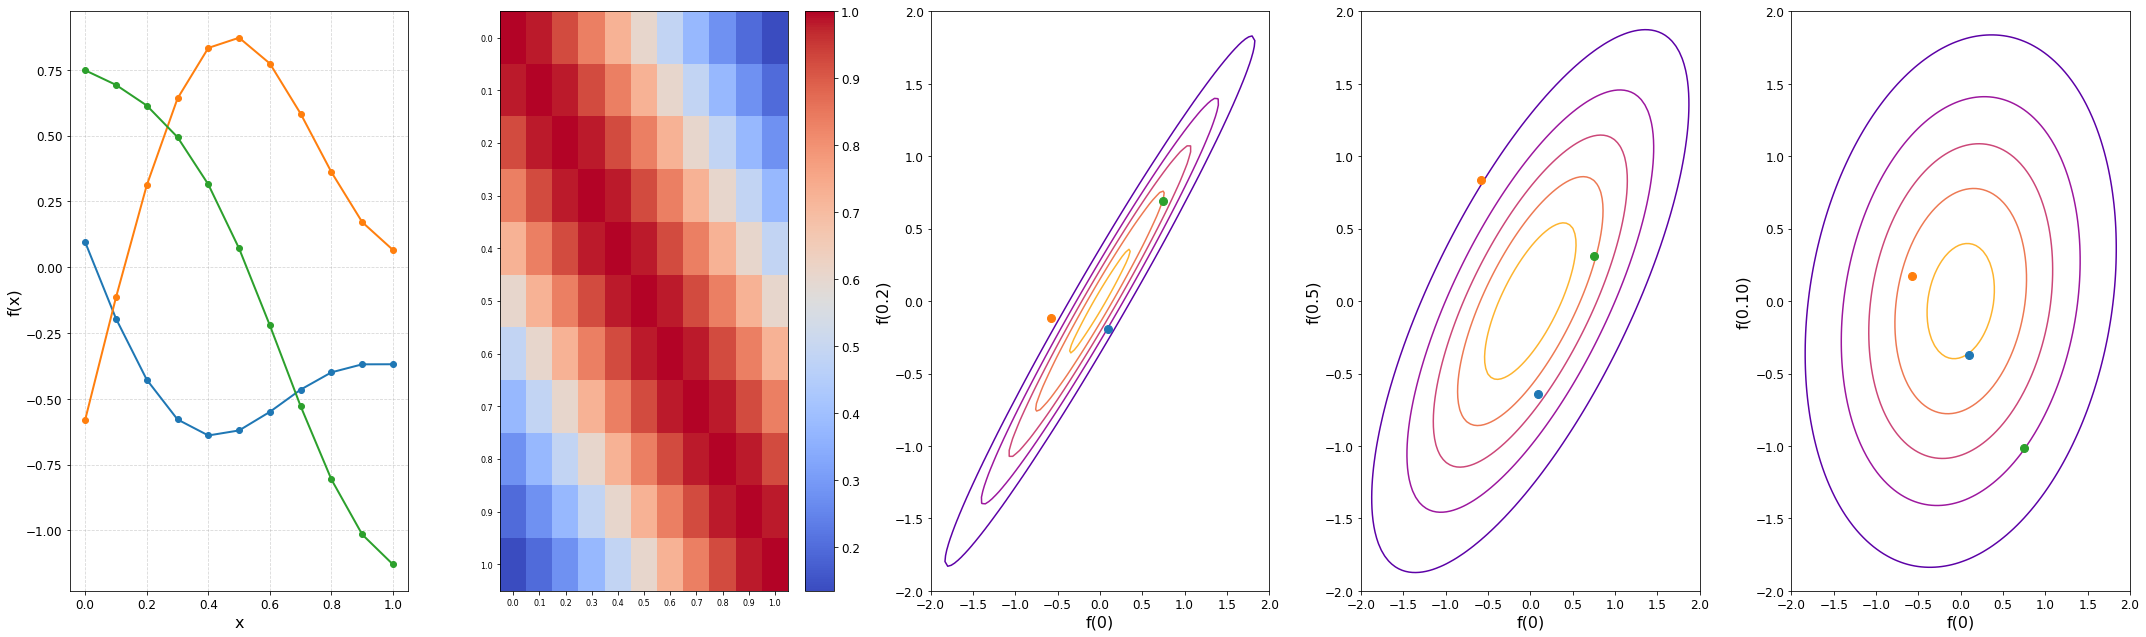
\includegraphics[width=1\textwidth]{LatexPlots/1dplots/Kernel_background.png}
        \caption{Sampling from the GP prior with zero mean and an RBF kernel ($\ell = 0.5$, $\sigma_f^2 = 1$). 
        The first plot shows three sample functions drawn from the prior distribution. 
        The second plot visualizes the covariance matrix as a heatmap, revealing the strength of correlations between inputs.
        The final three subplots display joint distributions between selected input pairs, illustrating how output correlation diminishes with increasing input distance.}
    \label{fig: samples_from_GP_prior}
\end{figure}


\noindent
We have discussed how the kernel function encodes the covariance structure of the GP prior. This structure depends on the choice of kernel. According to [\cite{bible}]
kernels can be divided into two major sub-groups, stationary kernels and non-stationary kernels. 
Stationary kernels depend only on the relative (often radial) distance between inputs \(\|x - x'\|\) and are invariant to translations 
in the input domain. By contrast, non-stationary kernels depend explicitly on 
the absolute values of \(x\) and \(x'\), allowing the function’s properties—such as smoothness 
or amplitude—to vary across the domain. For more detailed discussion on building, combining, and customizing these kernels, 
see \cite{kernelcookbook} and \cite[Ch.~4]{bible}.

\bigskip

\noindent
In Table~\ref{tab:kernel-examples}, we provide an overview of several common kernel types, 
showing both their functional form and samples drawn from the corresponding GP priors. 
While each kernel imposes a distinct structural pattern on the functions—such as smoothness, periodicity, or linearity—they are all similarly influenced by shared hyperparameters like the lengthscale. 
In addition, many kernels include unique internal parameters that further shape the behaviour of the modeled functions. 
In the following subsections, we explore each of these kernels in detail and discuss the role of their associated hyperparameters.


\begin{table}[H]
    \centering
    \renewcommand{\arraystretch}{4} % Slightly tighter rows
    \setlength{\tabcolsep}{2pt} % Tighter columns
    \small % Smaller text to fit content

    \begin{tabular}{|>{\centering\arraybackslash}m{2cm}|*{6}{>{\centering\arraybackslash}m{2.3cm}|}} 
        \hline
        \textbf{Kernel name:} & \textbf{RBF (SE)} & \textbf{Rational Quadratic} & \textbf{Periodic} & \textbf{Matern} & \textbf{Laplace} & \textbf{Linear (Dot Product)} \\ 
        \hline
        \textbf{Plot of $k(x, x')$:} & 
        \adjustbox{valign=c}{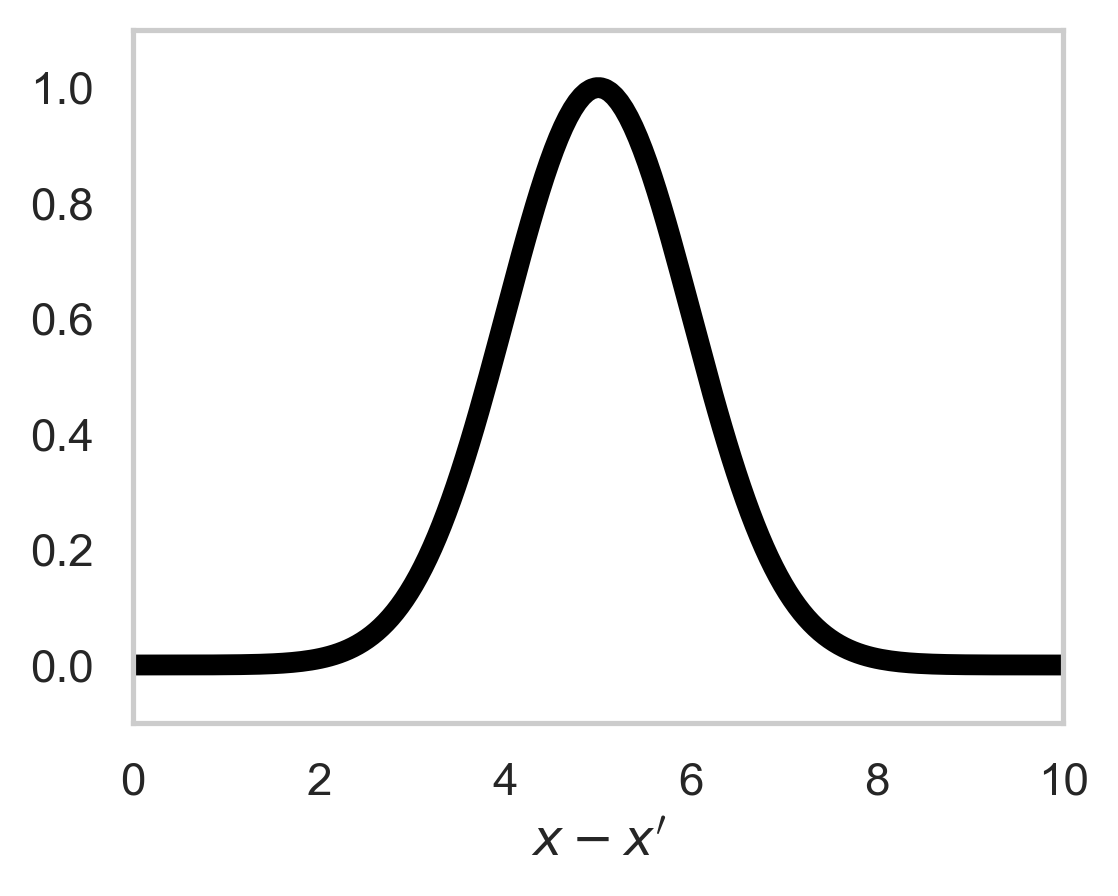
\includegraphics[width=2.25cm]{LatexPlots/1dplots/Kernel_RBF_SE.png}} & 
        \adjustbox{valign=c}{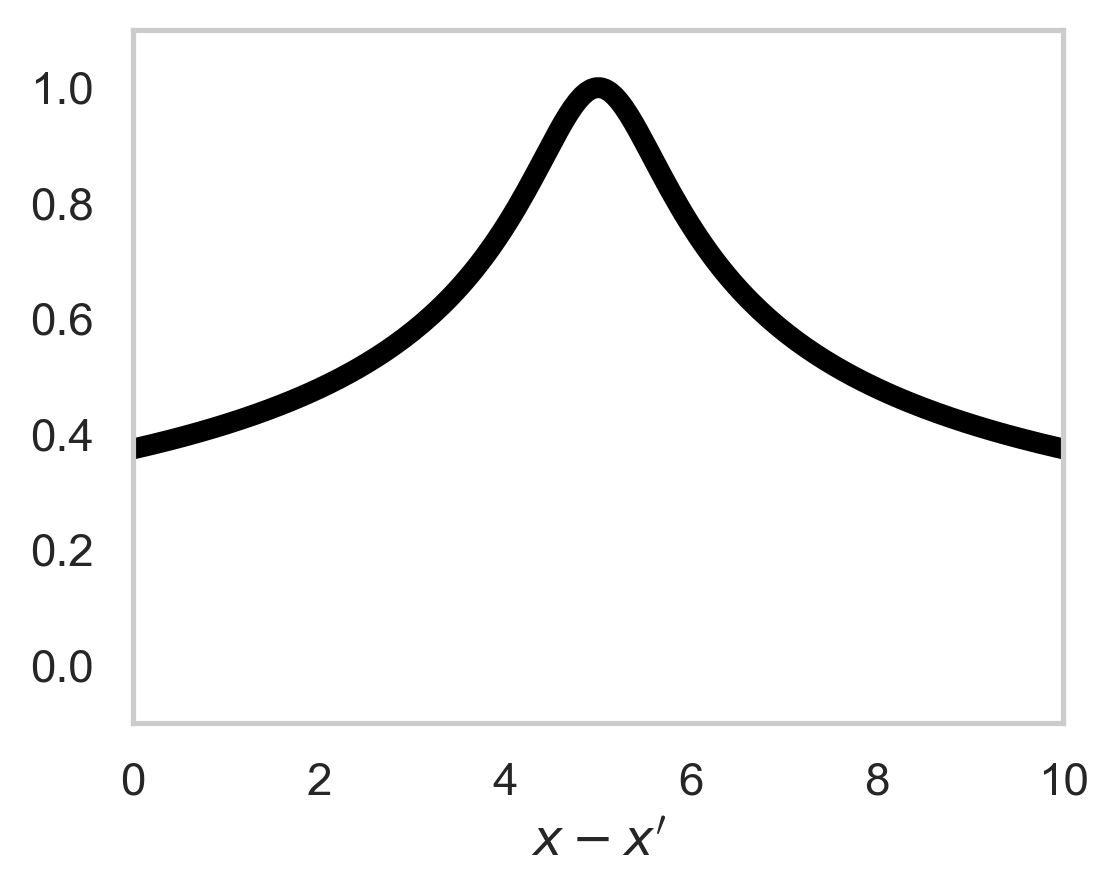
\includegraphics[width=2.25cm]{LatexPlots/1dplots/Kernel_Rational_Quadratic.png}} & 
        \adjustbox{valign=c}{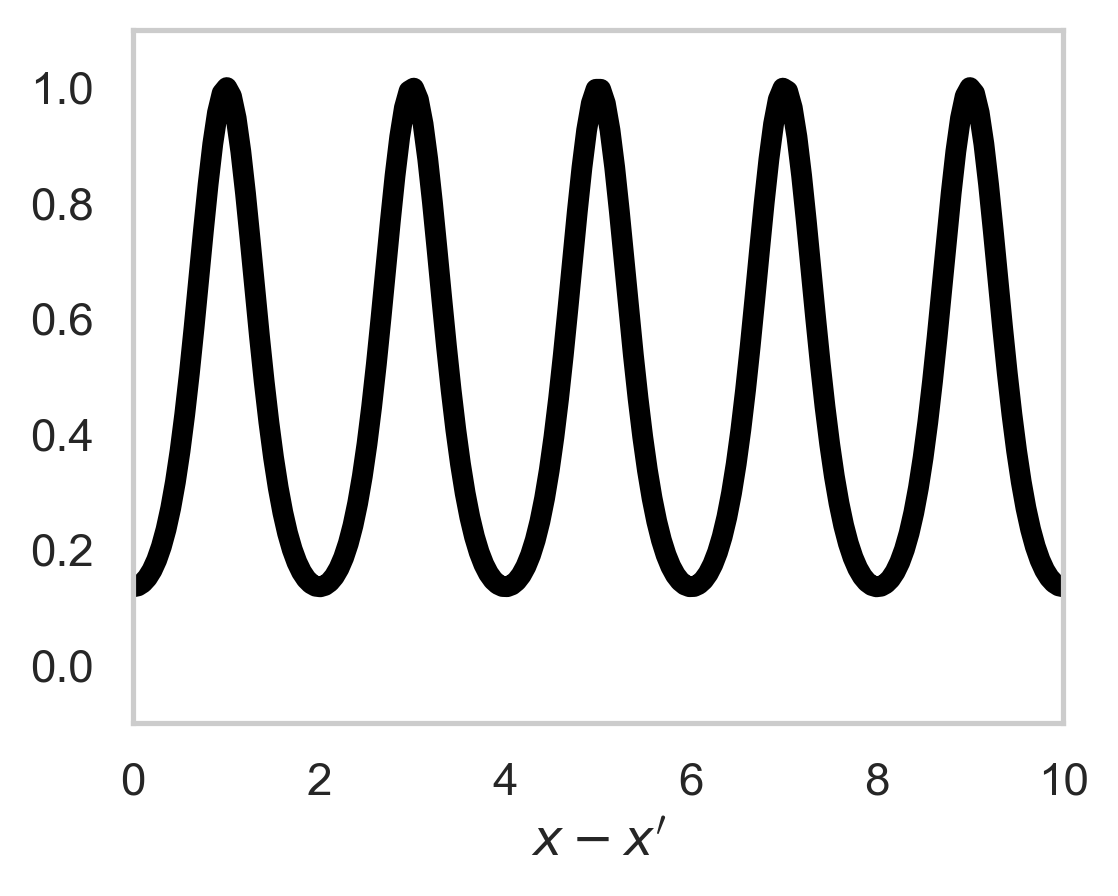
\includegraphics[width=2.25cm]{LatexPlots/1dplots/Kernel_Periodic.png}} & 
        \adjustbox{valign=c}{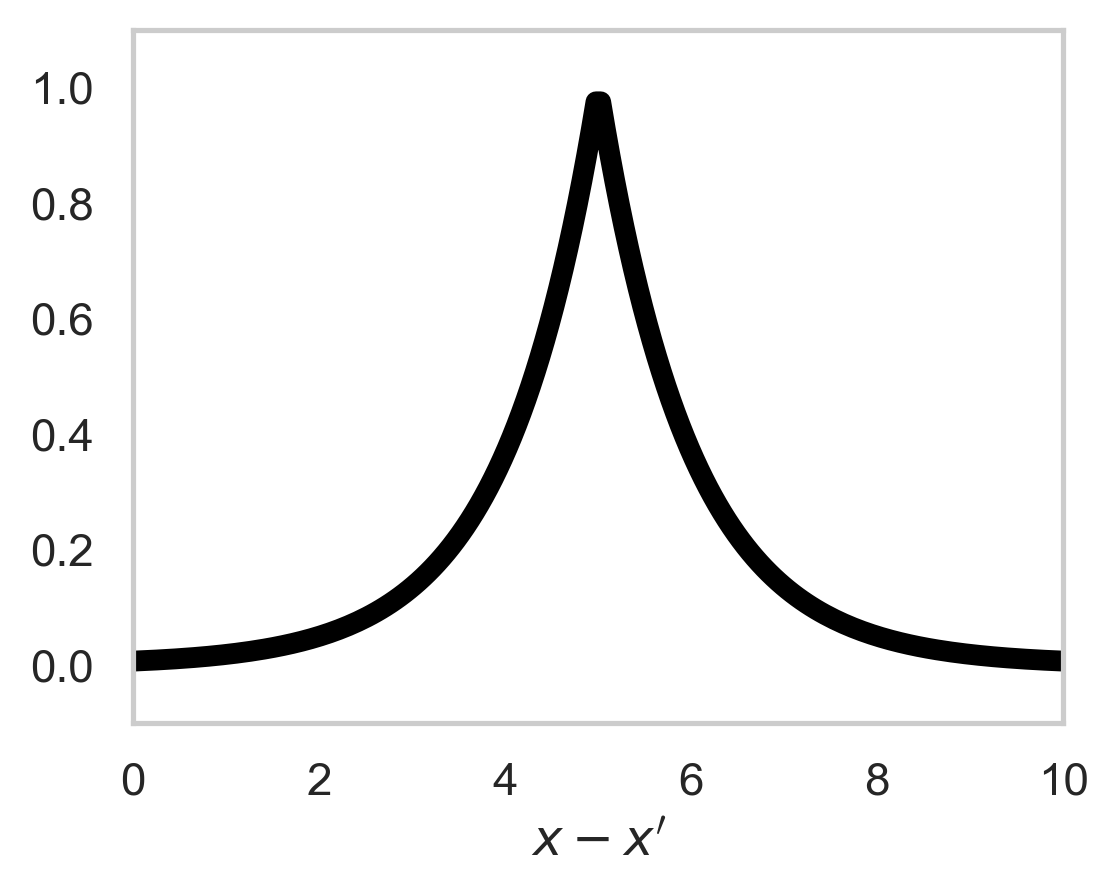
\includegraphics[width=2.25cm]{LatexPlots/1dplots/Kernel_Matern_nu05.png}} & 
        \adjustbox{valign=c}{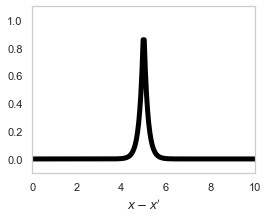
\includegraphics[width=2.25cm]{LatexPlots/1dplots/Kernel_Laplace_Exponential.png}} & 
        \adjustbox{valign=c}{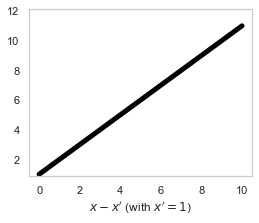
\includegraphics[width=2.25cm]{LatexPlots/1dplots/Kernel_Linear_Dot_Product.png}} \\ 
        \hline
        \textbf{GP Prior Samples:} & 
        \adjustbox{valign=c}{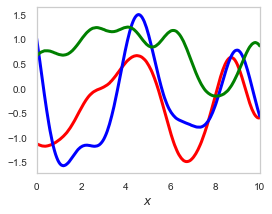
\includegraphics[width=2.25cm]{LatexPlots/1dplots/KernelSample_RBF_SE.png}} & 
        \adjustbox{valign=c}{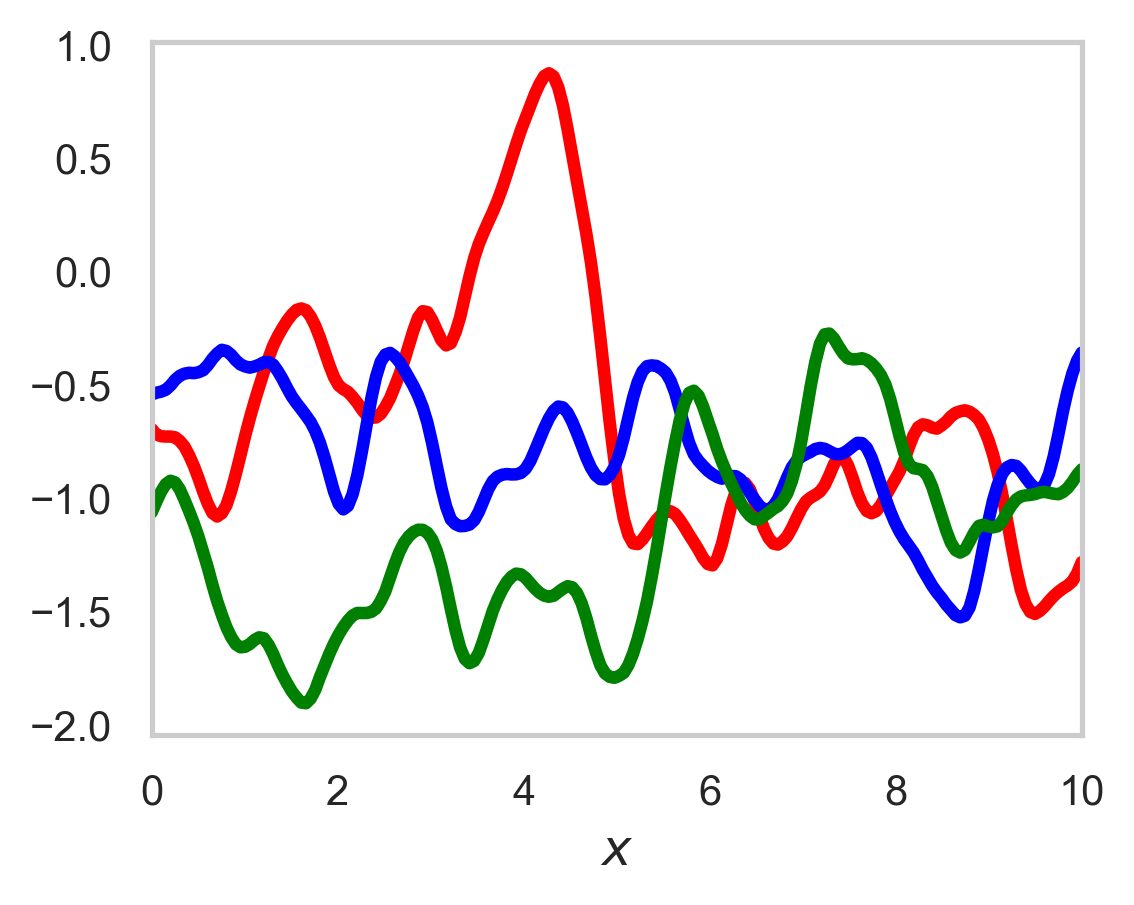
\includegraphics[width=2.25cm]{LatexPlots/1dplots/KernelSample_Rational_Quadratic.png}} & 
        \adjustbox{valign=c}{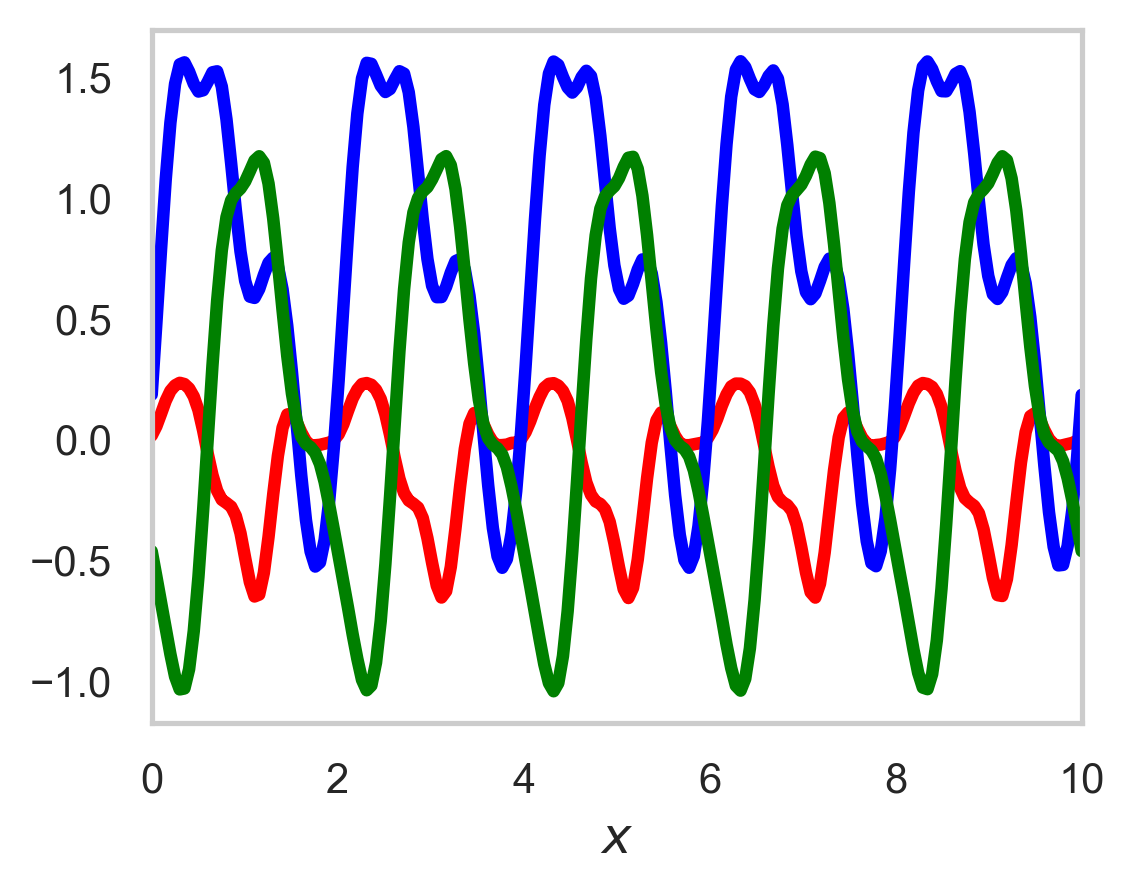
\includegraphics[width=2.25cm]{LatexPlots/1dplots/KernelSample_Periodic.png}} & 
        \adjustbox{valign=c}{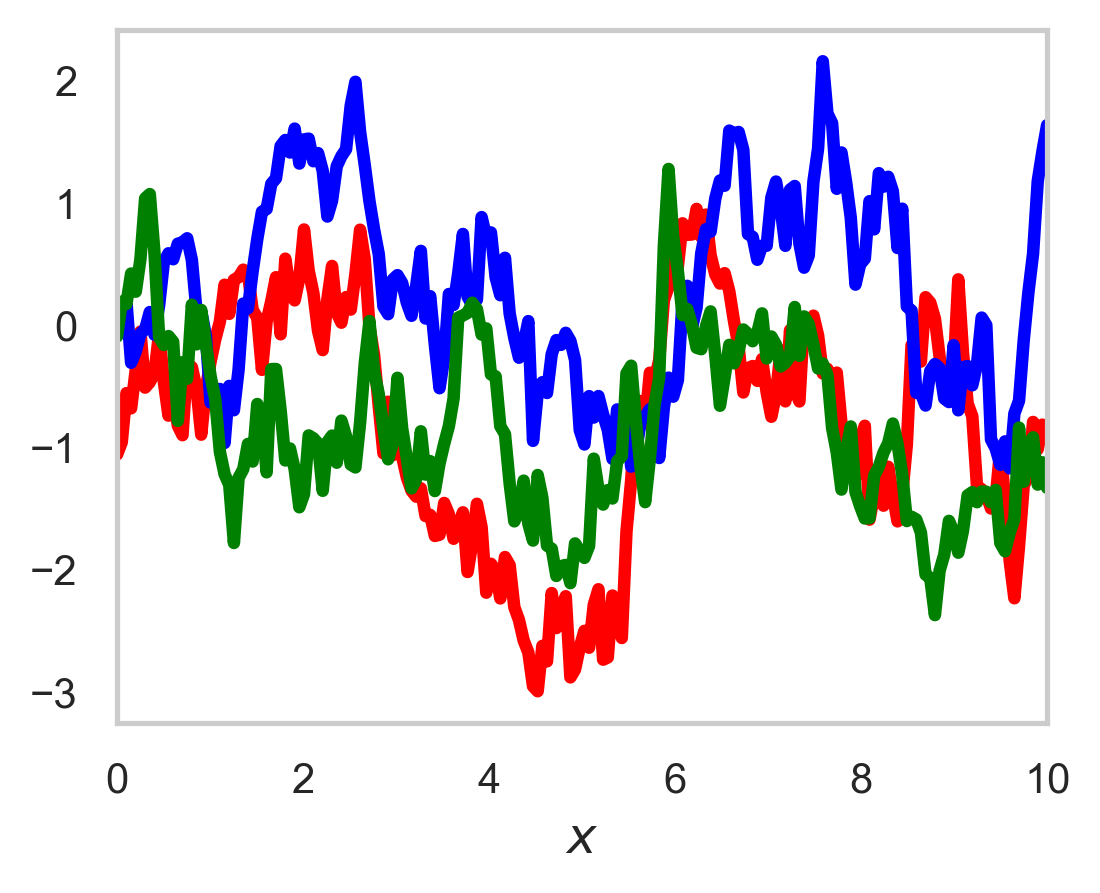
\includegraphics[width=2.25cm]{LatexPlots/1dplots/KernelSample_Matern_nu05.png}} & 
        \adjustbox{valign=c}{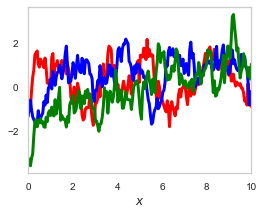
\includegraphics[width=2.25cm]{LatexPlots/1dplots/KernelSample_Laplace_Exponential.png}} & 
        \adjustbox{valign=c}{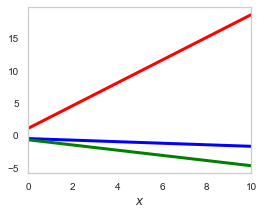
\includegraphics[width=2.25cm]{LatexPlots/1dplots/KernelSample_Linear_Dot_Product.png}} \\ 
        \hline
        \textbf{Key Hyperparameters} &
        $\ell$ (Lengthscale) &
        \shortstack{$\ell$ \\ $\alpha$ (Scale-mix)}&
        \shortstack{$\ell$ \\ $p$ (Period)} &
        \shortstack{$\ell$ \\ $\nu$ (Smoothness)} &
        $\gamma$ (Decay rate) &
        None or variance \\ 
        \hline
        \textbf{Structure type:} & 
        Local variation & 
        Multi-scale local variation & 
        Repeating structure & 
        Rough to smooth & 
        Rougher variation & 
        Linear functions \\ 
        \hline
    \end{tabular}
    \caption{
        Visual comparison of common kernel functions and their effect on Gaussian process priors. 
        Each column shows the kernel shape $k(x, x')$, samples from the corresponding GP prior, and a summary of the structure it imposes. 
        All kernels were evaluated using a lengthscale parameter $\ell = 1$ (except where noted). 
        For the Matern kernel, $\nu = 0.5$; Laplace kernel, $\gamma = 6$; Rational Quadratic kernel, $\alpha = 0.25$; and Periodic kernel, period $p = 2$.
        Detailed formula and graphs for each kernel are provided in the appendix \ref{appendix:B}.
        }
    \label{tab:kernel-examples}
\end{table}

\noindent
\Sean{Update}
Note: In practice, we scale each kernel by a signal variance hyperparameter \(\sigma_f^2\), which governs the overall vertical variation in the function.
This scaling is applied consistently across all kernel types and is discussed further in the \ref{sec: Handlingnoise}.

\noindent
From Table~\ref{tab:kernel-examples}, we observe that the RBF, Rational Quadratic, Matern, Laplace, and Periodic kernels are all examples of stationary kernels (i.e depend on $|x-x'|$). 
Many of these—such as the RBF, Matern,Rational Quadratic and Laplace—exhibit ``bell-shaped'' structures: inputs \(x\) and \(x'\) that are close together yield high covariance,
which then decays as the distance \(\|x - x'\|\) increases.The Periodic kernel, while also stationary, has a unique structure. Instead of decaying monotonically with distance, 
it assigns high covariance to inputs that are separated by integer multiples of a fixed period \(p\). This leads to a repeating pattern of similarity,
making the kernel ideal for modeling functions which are periodic.

\noindent
We have examined multiple kernel types and their properties.We will now briefly visualise and examine the effect of the lengthscale hyperparameter and 
the signal variance hyperparameter on the GP prior. We will use the RBF kernel as an example, but the same principles apply to other kernels.



\begin{figure}[H]
    \centering
        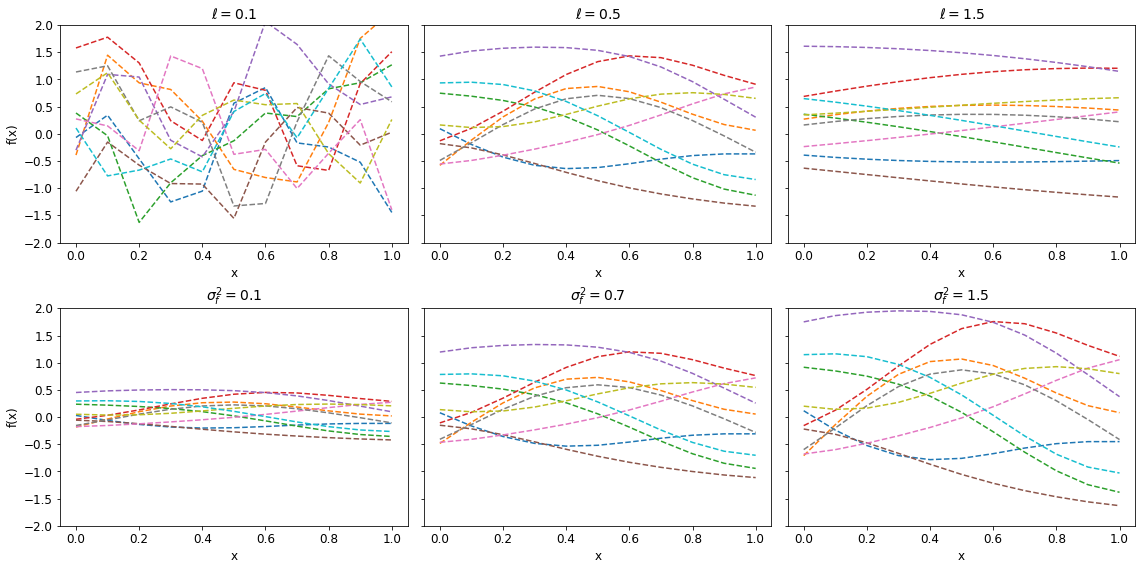
\includegraphics[width=\textwidth]{LatexPlots/1dplots/Kernel_hyperparams.png}
        \caption{Sampling from the GP prior with mean 0 and covariance given by the RBF kernel.
        The first plot shows the effect of the lengthscale hyperparameter \(\ell\) on the GP prior.We fix the signal variance to 1.
        The second plot shows the effect of the signal variance hyperparameter \(\sigma_f^2\) on the GP prior.We fix the lengthscale to 0.5.}
    \label{fig: GPprior_hyperparams}
\end{figure}

\Sean{Comment on how each effects prior. Below is waffle from a while ago could potentially add}

% \noindent
% It is evident that the choice of kernel hyperparameters has a significant impact on the shape of the posterior mean and its uncertainty.
% The RBF kernel with noise is given by:
% \[
% k(x, x') = \sigma_f^2 \exp\left( -\frac{(x - x')^2}{2\ell^2} \right) + \sigma_n^2 I,
% \]
% where $\ell$ controls the length scale, $\sigma_f^2$ represents the signal variance, and $\sigma_n^2$ denotes the noise level.

% \noindent
% From Figure~\ref{fig: GPprior_hyperparams}, we observe that a very small length scale $\ell \approx 0$ leads to overfitting:
% the GP closely tracks the training data, with sharp fluctuations between points. This occurs because the kernel's covariance rapidly decays with distance,
% making function values at different inputs nearly uncorrelated unless they are extremely close. As a result, the model fits the noise and exhibits a jagged appearance.
% In contrast, a large length scale such as $\ell \approx 3$ causes over-smoothing. Distant points remain highly correlated,
% producing a nearly linear mean function that fails to capture local variations. A moderate length scale ($\ell = 0.109$ in this case)
% provides a balance—producing a smooth yet flexible mean function that captures trends in the data without overfitting.

% \noindent
% Regarding the signal variance $\sigma_f^2$, we find that a very small value (e.g., $\sigma_f^2 \approx 0.01$) causes the GP mean to flatten,
% as the prior assumes the function to vary very little. As the variance increases (e.g., $\sigma_f^2 = 1.2$ and $\sigma_f^2 = 10$), the credible intervals widen slightly,
% but the overall mean function shape remains relatively stable. This suggests that posterior inference over $\sigma_f^2$ may exhibit considerable uncertainty, a point we explore further using MCMC sampling in Section \ref{sec: MCMC}.


% \noindent
% Lastly, varying the noise level $\sigma_n^2$ primarily affects the width of the credible interval, 
% while the mean function remains largely unchanged. As $\sigma_n^2$ increases, the model accounts for higher observation noise, 
% and uncertainty in the predictions increases accordingly. This relationship appears approximately linear in the visualizations.


\Sean{Could mention something about credible interval here, Maybe next section}
% \textbf{Credible Interval Behavior:} In Gaussian Process regression, the predictive variance at a new input $x^*$ is given by
% \[
% k(x^*, x^*) - k(x^*, X)(K_{XX}^{-1})k(X, x^*).
% \]

% With an RBF kernel, $k(x^*, X)$ will be near-zero if $x^*$ is farther than a few $\ell$'s away from all training inputs $X$. 
% For small $\ell$, this situation happens frequently – any point outside a tiny neighborhood of training data effectively has $k(x^*, X) 
% \approx 0$, so its predictive variance is roughly
% \[
% k(x^*, x^*) = \sigma_f^2
% \]
% (the prior variance). Thus, the 95\% credible interval reverts to roughly $\pm 2\sigma_f$ in large gaps or outside the data range.
% For large $\ell$, on the other hand, $k(x^*, X)$ remains sizable over a much broader range, reducing the variance term. The uncertainty
% only approaches the prior level far outside the data (several $\ell$'s away). In effect, a large $\ell$ flattens the covariance function
% so that the GP “remembers” the training set far out, maintaining narrower error bars over a wider domain.



\subsubsection*{Adding Data: Prior to Posterior}
\label{sec: priortoposterior}

We have discussed how our prior distribution is dependent on the choice of kernel and the hyper-parameters of said kernel. In this section
we will discuss how we can update our prior distribution \ref{eq: Multivariate prior} to achieve our new prediction distribution distribution from which we can make
inferences. One of the key strengths of Gaussian Processes is that, given observations at training inputs \(X\) and setting kernel hyper-parameters \(\theta\)
we can make predictive inferences about the function value at any new test location \(x_*\).
By applying the standard conditional Gaussian formulas (see appendix \Sean{Must clean up this derivation in appendix} \ref{appendix:A} for the full derivation),
the posterior distribution of \(f(x_*)\) given \(\{X, f(X)\}\) is Gaussian and given by:
%
\begin{subequations}
    \begin{equation}
    p\bigl(f(x_*) \mid f(X), X, X_*,\theta \bigr) 
    \sim \mathcal{N}\!\left(m(x_*),\;\sigma^2(x_*)\right),
    \label{eq: predictive_dist}
    \end{equation}
    \vspace{-8ex}
    \begin{align}
    m(x_*) 
    &= \mu(x_*) + k(x_*, X)\,k(X, X)^{-1}\left[f(X) - \mu(X)\right],
    \label{eq: predictive_mean} \\
    \sigma^2(x_*) 
    &= k(x_*, x_*) - k(x_*, X)\,k(X, X)^{-1}\,k(X, x_*).
    \label{eq: predictive_variance}
    \end{align}
\end{subequations}    
% 
In these expressions:
\begin{itemize}
    \item \( \mu(\cdot) \) is the mean function ( We take this to be zero since we centre the data prior to prediction),
    \item \( k(X, X) \) is the covariance matrix among the observed training points,
    \item \( k(x_*, X) \) is the vector of cross-covariances between the test point \(x_*\) and the training inputs,
    \item \( k(x_*, x_*) \) is the prior variance at the test point itself.
\end{itemize}

\noindent
We now have an analytic function that can be evaluated to find the mean function value and variance at any input point.
This is a very useful property that Gaussian Processes possess. Figure~\ref{fig: priortoposterior} shows how we update our
distributions based on the training points. We initially plot samples taken from the prior distribution (Equation~\ref{eq: Multivariate prior}). 
After conditioning this distribution on one training point and obtaining the new predictive posterior distribution (Equation~\ref{eq: predictive_dist}), 
we see that the predictive mean passes exactly through the training point, has small variance around it, and then fans out farther away. 
Conditioning on two training points at opposite ends of our input domain creates an ellipse-shaped credible interval whose largest radius 
appears midway between the two training points. With more training points, the predictions align progressively closer to the true function 
and the variance becomes smaller.

\noindent
Note that this example uses a one-dimensional, noise-free function and a basic RBF kernel with fixed hyperparameters (\(\ell = 1\), \(\sigma^2 = 0.5\)). 
In practice the choice of Kernel function plays a pivotal role in the assumptions we make about the shape and general behaviour of our model. In the next section
we examine the different kernel choices available and the assumptions that each kernel encodes about our function structure, such as smoothness and periodicity.



\begin{figure}[H]
    \centering
    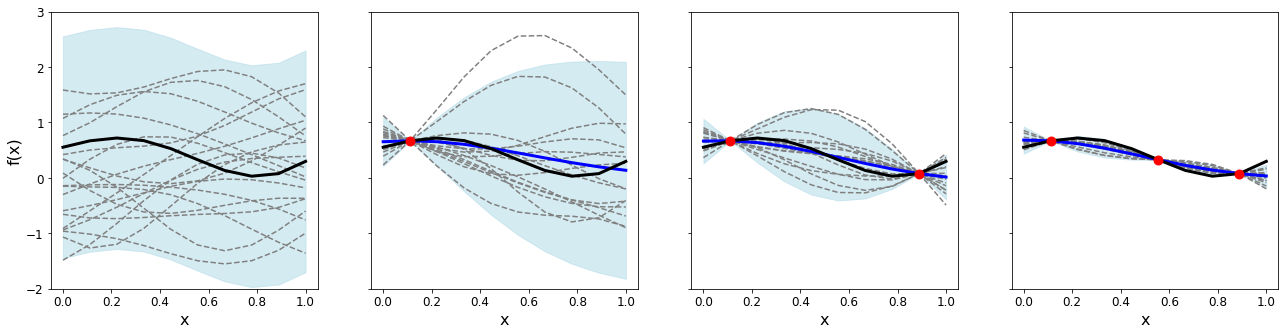
\includegraphics[width=\textwidth]{LatexPlots/1dplots/priortoposterior.png}
    \caption{1D Gaussian Process Regression: Prior to Posterior. This sequence shows how the GP prior transforms into a posterior as more data points are added. 
    The RBF kernel was used with hyper-parameters: $l = 1$, $\sigma^2 = 0.5$.The black line represents the true function. The blue is the mean of each posterio distribution. 
    The light blue shaded region is the credible interval and the grey lines are the samples drawn from each posterior/prior. }
    \label{fig: priortoposterior}
\end{figure}
\Sean{can add a potential link to animation here illustrating the nice distribution formed at each point}




\subsection{Handling Noise in our Data}
\label{sec: Handlingnoise}

So far, our discussion has assumed noise-free observations. However, real-world data is rarely clean, measurements often include some form of uncertainty. To make our Gaussian Process models more applicable to this real-world data,
we now explore how to incorporate noise into the GP framework.

\bigskip

\noindent
We assume that each observation includes the true function value plus Gaussian noise:
\begin{equation}
y_i = f(x_i) + \epsilon_i, \quad \epsilon_i \sim \mathcal{N}(0, \sigma_{n,i}^2),
\end{equation}
where \( \sigma_{n,i}^2 \) is the noise variance associated with input \( x_i \). This allows us to model both homoscedastic and heteroscedastic noise under a unified notation.

\bigskip

\noindent
Under this model, we have the following Gaussian assumptions:
\begin{align}
f &\sim \mathcal{N}(0, K), &&\text{(prior over the true function)} \\
y &\sim \mathcal{N}(0, K + \Sigma), &&\text{(distribution over noisy observations)},
\label{eq: prior_distribution_noise}
\end{align}
where \( \Sigma = \mathrm{diag}(\sigma_{n,1}^2, \sigma_{n,2}^2, \dots, \sigma_{n,n}^2) \) is the noise covariance matrix.

\bigskip
\noindent
This now updates our previous posterior mean and variance (eq: \ref{eq: predictive_mean} and \ref{eq: predictive_variance}) to a revised posterior:
%
%
\begin{subequations}
\begin{align}
    P(f_*|X,X_*,\theta,y) &\sim \mathcal{N}(m(f_*), \text{Var}(f_*))
    \label{eq: predictive_distribution_noise},\\
m(f_*) &= K_*^T (K_y)^{-1} y,
\label{eq: predictive_mean_noise}\\
\text{Var}(f_*) &= K_{**} - K_*^T (K_y)^{-1} K_*,
\label{eq: predictive_variance_noise}
\end{align}
\end{subequations}
%
%
where \(K_y\) depends on how we handle our noise. There are three main cases of how we handle our noise

\subsubsection*{Homoscedastic Noise} 

In the homoscedastic case, we assume that all observations have the same noise level, meaning the noise variance is constant across the dataset:
\[
\sigma_{n,i}^2 = \sigma_n^2 \quad \forall i.
\]
This simplifies the noise covariance matrix \( \Sigma \) to a scalar multiple of the identity matrix:
\[
\Sigma = \sigma_n^2 I.
\]
The total covariance matrix of the observed data becomes:
\[
K(X, X) + \sigma_n^2 I = 
\begin{bmatrix}
k(x_1, x_1) + \sigma_n^2 & \cdots & k(x_1, x_n) \\
\vdots & \ddots & \vdots \\
k(x_n, x_1) & \cdots & k(x_n, x_n) + \sigma_n^2
\end{bmatrix}.
\]
Our prior distribution now becomes:
\begin{equation}
y \sim \mathcal{N}(0, K+\sigma_n^2 I)
\label{eq: prior_withnoise}
\end{equation}
where $\sigma_n^2$ is a new parameter which effects the shape of the distribution. In figure \ref{fig: GPprior_hyperparams} we 
explored how the internal kernel hyper-parameters effect the shape of the sampes from our prior distribution. We now examin how the noise (i.e $\sigma_n^2$) effects samples from our prior distribution from \ref{eq:  predictive_distribution_noise}.
Our predictive distribution remains as in \ref{eq: predictive_distribution_noise}

\begin{figure}[H]
    \centering
        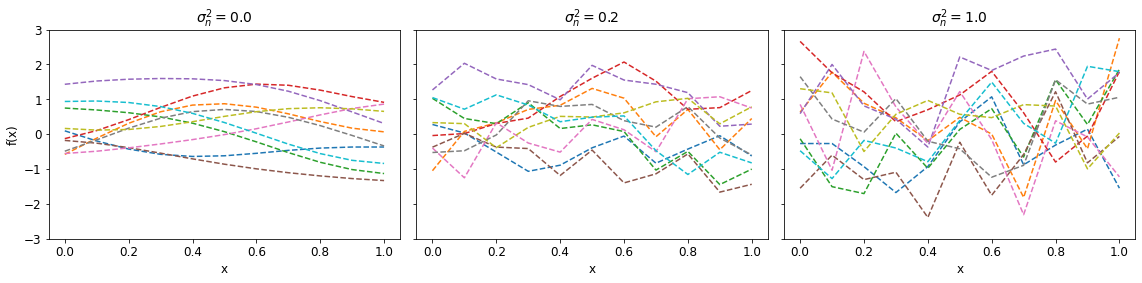
\includegraphics[width=\textwidth]{LatexPlots/1dplots/Kernel_noise.png}
        \caption{Sampling from the GP prior with mean 0 and covariance given by the RBF kernel.
        The plot shows the effect of the noise hyperparameter \(\sigma_n^2\) on the GP prior.We fix the signal variance to 1 and length scale to 0.5.}
    \label{fig: kernel_noise}
\end{figure}
\noindent
Our posterior distribution is as in eqn \ref{eq:  predictive_distribution_noise} with \(K_y = K(X, X) + \sigma_n^2 I \) for some constant \(\sigma_n\)


\subsubsection*{Heteroscedastic Noise}  
\textbf{Known Noise:}
%
In this case, the noise variance changes across the input space—some observations are noisier than others. If we know the individual noise variances \( \sigma_i^2 \) for each training input \( x_i \), we incorporate them by adding a diagonal noise matrix to the kernel:
\[
K(X, X) + \Sigma = 
\begin{bmatrix}
k(x_1, x_1) + \sigma_1^2 & \cdots & k(x_1, x_n) \\
\vdots & \ddots & \vdots \\
k(x_n, x_1) & \cdots & k(x_n, x_n) + \sigma_n^2
\end{bmatrix},
\]
where \( \Sigma = \text{diag}(\sigma_1^2, \sigma_2^2, \dots, \sigma_n^2) \).
In this case the noise is not found as a hyper-parameter but instead just added to the diagonal of the covariance matrix.
Our posterior distribution is as in eqn \ref{eq:  predictive_distribution_noise} with \(K_y =K(X, X) + \Sigma \) where \(\Sigma\) is the known noise of our data. 

\vspace{1em}
\noindent
\textbf{Learning Noise over the Input Space:}
%
If the noise variance is unknown but varies across the input space, we can model it as a function. 
This is done by building a kernel that captures both smooth, global trends and rough, local fluctuations. 
In practice, this means building an additive kernel made up of sub-kernels.For example, as seen in Table~\ref{tab:kernel-examples}, some kernels like the Matern, Laplacian, or Rational Quadratic capture local variations well (interpreted as noise),
while others like the RBF capture broader, smoother structure. By combining these, we can allow one kernel component to model the general structure of the function, and the other to model the heteroscedastic noise behavior. 
Our posterior distribution is as in eqn \ref{eq:  predictive_distribution_noise} with :

\begin{equation}
    K_y = \theta_1 K_1(X, X) + \theta_2 K_2(X, X),
    \label{eq:additive_kernel}
\end{equation}
where \( K_1 \) and \( K_2 \) are distinct kernels chosen to capture different aspects of the data. 
The coefficients \( \theta_1 \) and \( \theta_2 \) are parameters that control the relative contribution of each kernel component.

\subsubsection*{Monte Carlo Sampling of Noise}  

This technique can be applied in both homoscedastic and heteroscedastic noise settings. Rather than explicitly modelling observation noise by adding a noise term to the kernel matrix, we instead account for uncertainty by perturbing the observed outputs with sampled noise.
Assuming Gaussian noise, we generate multiple noisy versions of the observed data by sampling from our noise distribution defined by the known noise. For each of these sampled datasets, we compute a Gaussian Process posterior, and then average the predictions to obtain a final predictive distribution that integrates over observation noise.
This Monte Carlo-style approach allows uncertainty in the outputs to be naturally incorporated into the predictions without modifying the covariance structure directly. A full mathematical description of this method is provided in Appendix~\ref{appendix:monte_carlo}.

%
%
\subsubsection*{Comparing Noise Models}
From Figure~\ref{fig:noise_comparison} we see how different noise assumptions influence samples drawn from the Gaussian Process prior. 
In the homoscedastic case (left), our samples exhibit consistent fluctuations across the entire domain due to a constant noise variance applied uniformly to all inputs. 
The heteroscedastic case (middle) introduces input-dependent noise, this results in regions of smoothness followed by abrupt variations—reflecting the fact that each output has its own associated noise level.
Finally, in the Monte Carlo noise sampling approach (right), we generate multiple samples by adding different levels of noise to our prior distribution on our true function values.
This highlight all the plausible functions consistent with the observed data and captures the full range of uncertainty introduced by noisy observations.

\begin{figure}[H]
    \centering
    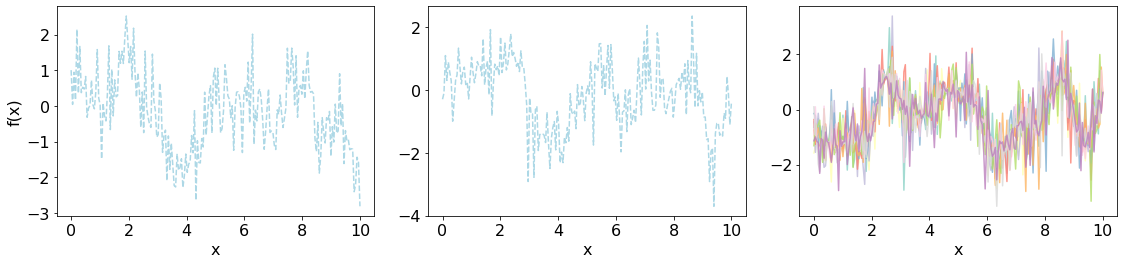
\includegraphics[width=\textwidth]{LatexPlots/1dplots/GPR_noise_comparison.png}
    \caption{Samples drawn from a zero-mean Gaussian Process prior with varying noise assumptions.
    \textbf{Left:} Homoscedastic noise, where a constant noise variance \(\sigma_n^2 = 0.5\) is added uniformly across all inputs.
    \textbf{Middle:} Heteroscedastic noise, where individual noise variances \(\sigma_i^2\) are known and drawn from \(\mathcal{N}(0, 0.5)\), resulting in a diagonal noise covariance.
    \textbf{Right:} Monte Carlo sampling of noisy observations, where multiple noisy realizations are generated from \(\mathcal{N}(f(x), \epsilon^2)\)}
    \label{fig:noise_comparison}
\end{figure}




\subsection{Hyper-parameters}
\label{sec: Hyper_parameters}
Until now, all predictive distributions such as Equations~\ref{eq: predictive_distribution_noise} and~\ref{eq: predictive_dist} have been conditioned on fixed kernel hyperparameters. As demonstrated in Figures~\ref{fig: GPprior_hyperparams} and~\ref{fig: kernel_noise}, these hyperparameters have a significant influence on the structure and behaviour of the Gaussian Process, shaping both the prior and posterior distributions. 
In practice, these hyperparameters are not known and must be inferred from the data. To do so, we aim to find the set of hyperparameters that best explain the observed data by maximising the log marginal likelihood, a method detailed in [Ch5\cite{bible}.]

\noindent
As outlined in Section~\ref{sec: Handlingnoise} we have different methods of handling noise resulting in different hyper-parameters to be optimised. We will focus on the general case here which can be easily manipulated for each spefici method.
From Equation~\ref{eq: prior_withnoise}, we have:
\[
y \sim \mathcal{N}(0, K + \Sigma I),
\]
where \( K \) is the kernel matrix computed from the training inputs \( X \), and \( \Sigma\) is the noise variance.

\noindent
This implies that the marginal likelihood which is the probability of the observed outputs \( y \) given the inputs \( X \) and hyperparameters \( \theta \)) is given by the multivariate Gaussian density. 

\[
p(y \mid X, \theta) = \frac{1}{(2\pi)^{n/2} |K_y|^{1/2}} \exp\left( -\frac{1}{2} y^\top K_y^{-1} y \right)
\]
where \( K_y = K + \Sigma I \), and \( \Sigma \) may be constant or input-dependent depending on the noise model used.
\noindent
The hyperparameters are given by:
\[
\theta = \left\{ \sigma_f^2, \ell, \text{(other internal kernel params)}, \sigma_n^2 \,\, \text{(if noise is modelled as a hyperparameter)} \right\}.
\]
\noindent
Taking the logarithm of this expression yields the \textit{log marginal likelihood}:
\begin{equation}\label{eq: 5}
\log p(y \mid X, \theta) = -\frac{1}{2} y^\top K_y^{-1} y - \frac{1}{2} \log |K_y| - \frac{n}{2} \log 2\pi
\end{equation}
\noindent
Our goal is to maximise this log marginal likelihood with respect to the hyperparameters \( \theta \), which typically includes the kernel lengthscale, signal variance, and noise variance. Once optimal values are found, we can use them to make accurate posterior predictions.
\Sean{Explain the below Figure~\ref{figure: Optimising Hyper-params}}
\begin{figure}[H]
    \centering
    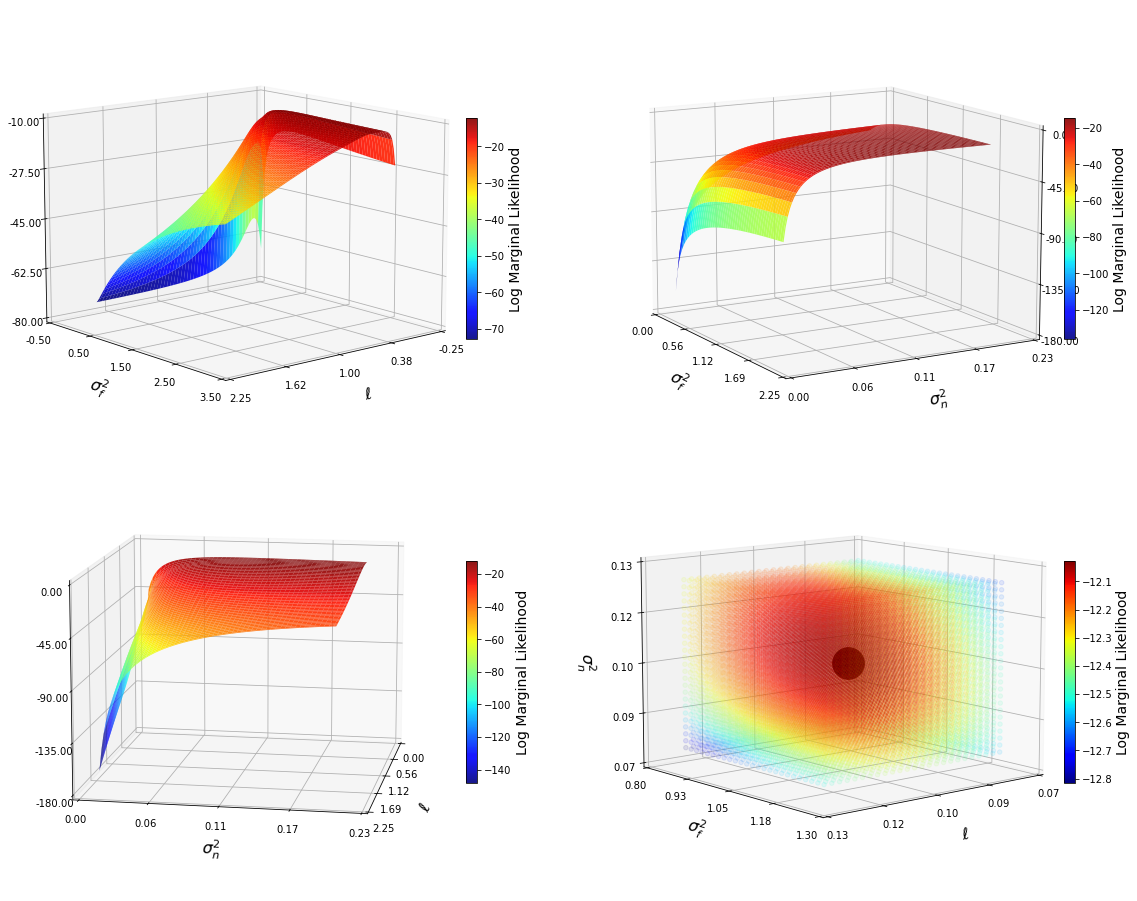
\includegraphics[width=0.8\textwidth]{LatexPlots/1dplots/LogLikeallparams.png}
    \caption{For a GPR with noise where we have the noise as a hyper-parameter we are forced to optimise a length hyper-parameter, a variance hyper-parameter and a noise hyper-parameter. 
    Here we have kept one parameter constant on each graph and compared the log likelihood space varying the other two parameters. 
    In the upper left panel the noise is set to $\sigma^2_n= 0.1$, in the upper right panel the length is set at $ \ell=0.5$, in the lower left panel the variance is set at $\sigma^2_f=1.5$. 
    In the final panel we plot a 3-dimensional scatter plot and illustrate the point estimate given by the optimisation algorithm as the black dot. This point is located at
    $(\sigma^2 = 1.16, l = 0.109$ noise$ = 0.105)$.}
   \label{figure: Optimising Hyper-params}
\end{figure} 


\section{Quantifying Uncertainty}
\label{sec: MCMC}
We have previously discussed the role of kernels and how their hyperparameters influence the shape of both the prior and posterior predictive distributions. As shown in Figure~\ref{figure: Optimising Hyper-params}, optimising hyperparameters does not necessarily yield a single “best” solution. 
Instead, there often exists a region of hyperparameter values that explain the data equally well, resulting in a flat or multi-modal log marginal likelihood surface.
Up to this point, the models considered have relied on point estimates—selecting the hyperparameters that maximise the log marginal likelihood and using them directly for prediction. 
While convenient, this approach ignores the underlying uncertainty across hyperparameters that achieve similarly high likelihood scores. To account for this, we now aim to construct a posterior distribution over the hyperparameters, thereby enabling us to quantify and visualise uncertainty in their values.

\noindent
Whereas previously we maximised the log marginal likelihood (see Equation~\ref{eq: 5}) to obtain a point estimate, we now turn to a fully Bayesian treatment. We seek the posterior distribution over hyperparameters \( \theta \), 
given the data \((X, y)\), expressed as:

\begin{equation}
p(\theta \mid y, X) = \frac{p(y \mid X, \theta) \, p(\theta)}{p(y \mid X)}
\end{equation}
where:
\begin{itemize}
    \item \( p(y \mid X, \theta) \) is the likelihood of the data given the hyperparameters,
    \item \( p(\theta) \) is the prior distribution over the hyperparameters,
    \item \( p(y \mid X) = \int p(y \mid X,\theta)p(\theta)d\theta \) is the marginal likelihood, serving as a normalising constant.
\end{itemize}
Since \( p(\mathbf{y} \mid X) \) is often intractable (unable to analytically intergate), we sample from the unnormalised posterior using MCMC:
\begin{equation}
p(\theta \mid \mathbf{y}, X) \propto p(\mathbf{y} \mid X, \theta) \, p(\theta)
\end{equation}
%
%
Using MCMC, we generate samples \( \{\theta^{(s)}\}_{s=1}^S \sim p(\theta \mid y, X) \) from this posterior.
From these samples we can then build a KDE to help visualise the distribution of our hyper-parameters. An example of this is done in figure~\ref{fig:MCMCresults}.
\begin{figure}[H]
    \centering
    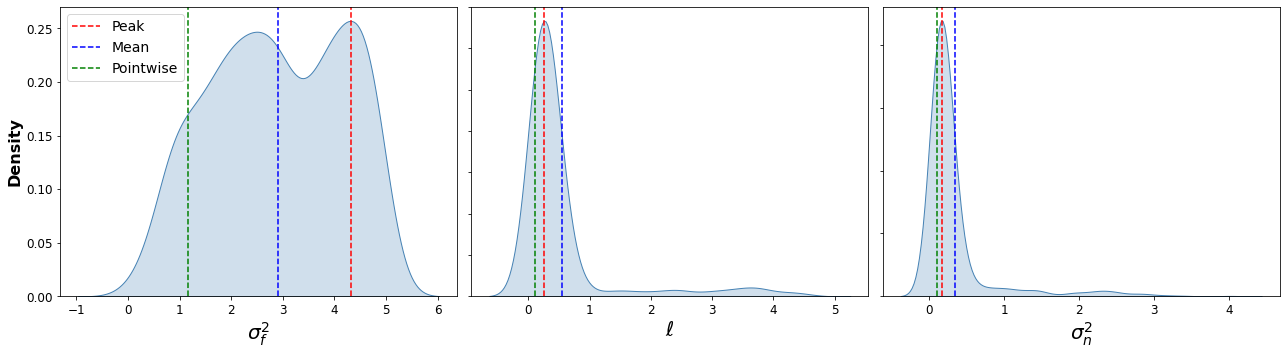
\includegraphics[width=\textwidth]{LatexPlots/1dplots/MCMCdistribution.png}
    \caption{
    Results from an MCMC run using a Gaussian Process Regression model with an RBF kernel and a WhiteKernel to model noise. We plot the Kernel density estimates of the posterior distributions for each hyperparameter, constructed from the sampled chains in our MCMC sampling. 
    the vertical red, blue and green lines indicate peak, mean, and pointwise estimates respectively.}
    \label{fig:MCMCresults}
\end{figure}
\noindent
We observe in Figure~\ref{fig:MCMCresults} that the posterior for the signal variance hyperparameter is nearly bimodal, with significant differences between the mean, mode, and point estimates. 
In these cases, relying on a single point estimate would lose critical information about model uncertainty.
To address this, we incorporate hyperparameter uncertainty directly into the predictive distribution by marginalising over the posterior \( p(\theta \mid y, X) \).
%
\begin{equation}
p(f_* \mid \mathbf{y}, X, X_*) = \int p(f_* \mid \mathbf{y}, X, X_*, \theta) \, p(\theta \mid \mathbf{y}, X) \, d\theta.
\end{equation}
Since this integral is also often intractable we approximate the marginalised predictive distribution via MCMC samples \( \{\theta^{(s)}\}_{s=1}^S \):
%
\begin{equation}
p(f_* \mid \mathbf{y}, X, X_*) \approx \frac{1}{S} \sum_{s=1}^{S} p(f_* \mid \mathbf{y}, X, X_*, \theta^{(s)}).
\end{equation}
%
The resulting mean and variance are computed using the law of total variance:
%
\begin{equation}
\mathbf{E}[f_*] \approx \frac{1}{S} \sum_{s=1}^{S} \mu^{(s)}(f_*), \quad
\text{Var}[f_*] \approx \frac{1}{S} \sum_{s=1}^{S} \left[ \sigma^{2(s)}(f_*) + \left(\mu^{(s)}(f_*)\right)^2 \right] - \left( \mathbf{E}[f_*] \right)^2.
\end{equation}
This procedure allows the final predictive distribution to reflect both data noise and model uncertainty.


\section{Multi-Dimensional GPR}

To model functions with multiple input dimensions, a common and flexible approach is to construct kernels that operate over each input dimension individually, 
and then combine them using a product. For example, multiplying RBF kernels defined on each input dimension yields a multi-dimensional RBF kernel.
A specific case of this is the RBF-ARD (Automatic Relevance Determination) kernel, which assigns a separate lengthscale parameter \( \ell_d \) to each input dimension \( d \):

\[
k(\mathbf{x}, \mathbf{x}') = \sigma_f^2 \exp\left( -\frac{1}{2} \sum_{d=1}^D \frac{(x_d - x'_d)^2}{\ell_d^2} \right)
\]

\begin{figure}[H]
    \centering
    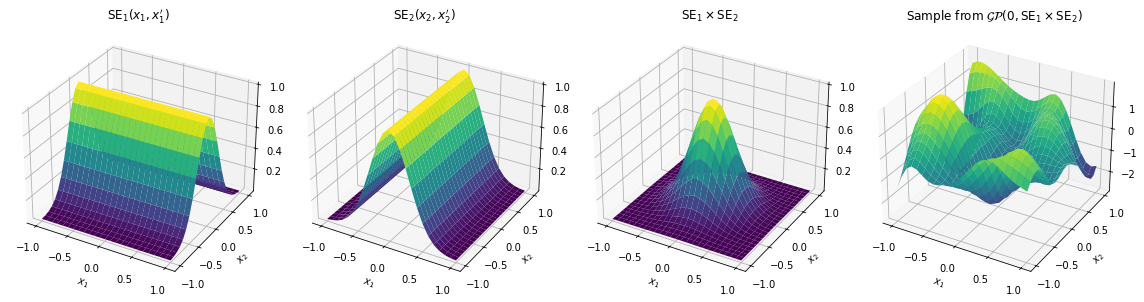
\includegraphics[width=\textwidth]{LatexPlots/final_gps_plots/2dkernels.png}
    \caption{
    Visualisation of constructing a two-dimensional kernel by multiplying two one-dimensional RBF kernels, each operating on a separate input dimension. Both kernels use a length scale of \(\ell = 0.3\). 
    The resulting product kernel models smooth interactions across both dimensions, and a sample drawn from the corresponding GP prior is shown.}
    \label{fig:2dkernels}
\end{figure}


\section{Method}
\begin{figure}[H]
    \centering
   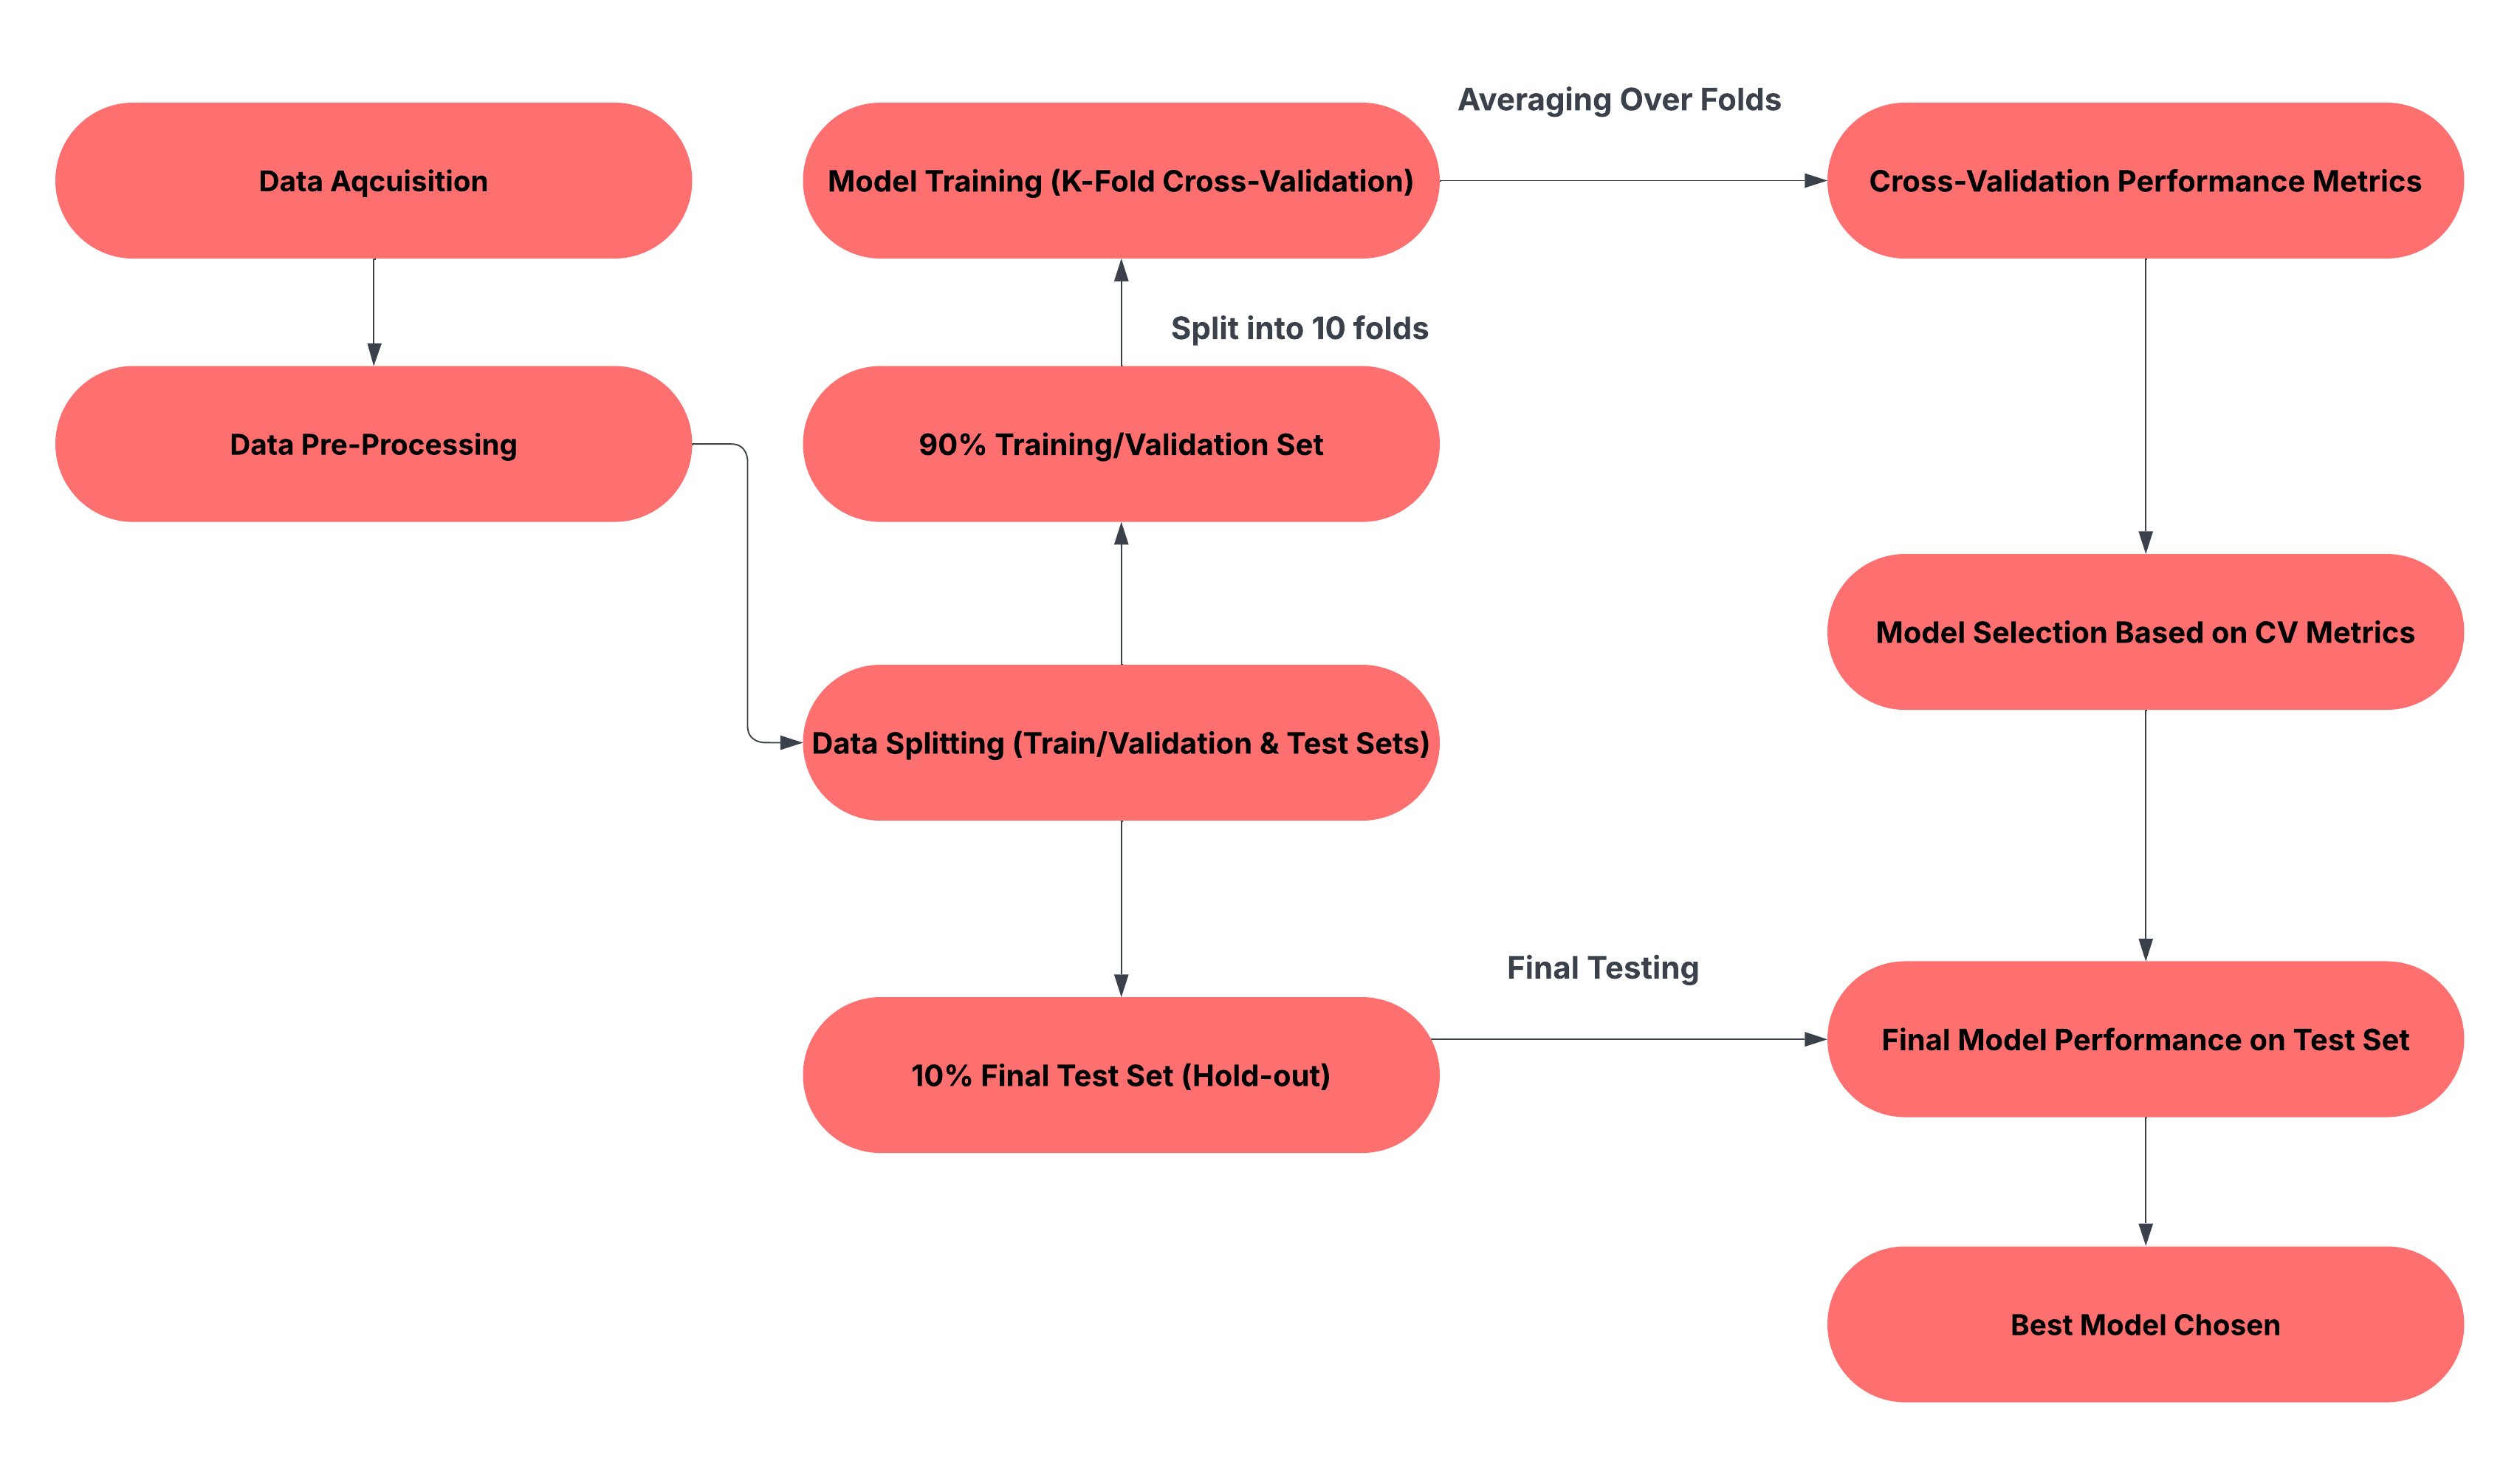
\includegraphics[width=0.8\textwidth]{LatexPlots/Flowchart.png}
    \caption{Method Flow Chart}
    \label{fig:flowchart}
\end{figure}
\subsection{The Models}
\label{subsec:Models}
To build a robust Gaussian Process Regression (GPR) model, I constructed a comprehensive set of model configurations by combining the kernels described in Section~\ref{sec: Kernels} with the noise-handling techniques introduced in Section~\ref{sec: Handlingnoise}. 
A full summary is provided in Table~\ref{tab:model_summary}. Below, we outline the different classes of models explored:

\noindent
\textbf{Homoscedastic Noise Models}
\begin{itemize}
    \item \textbf{White Kernel:} Noise is modelled as a global hyperparameter using the \texttt{WhiteKernel} class added to each kernel. After initial examination I found that the results of optimising the noise hyper-parameter varied massively with the noise bounds. 
    To get a full picture of the noise hyper-paraters I implemented three variants of this model with different noise bounds:
    \begin{itemize}
        \item \texttt{whitenoerror}: loose bounds \((10^{-6}, 10^6)\),
        \item \texttt{whiteminmaxerror}: bounds set using the 5th and 95th percentiles of the known standard deviations,
        \item \texttt{whitemeanerror}: bounds centered around the mean known uncertainty.
    \end{itemize}
\end{itemize}
%
%

\noindent
\textbf{Heteroscedastic Noise Models}
\begin{itemize}
    \item \textbf{Known Noise:} The \texttt{fixedalpha} model assumes noise variance is known at each input and adds this directly into the kernel diagonal using the \texttt{alpha} argument of \texttt{GaussianProcessRegressor}.
    \item \textbf{Monte Carlo Sampling:} The \texttt{montecarlo} model accounts for our observed mismatch values not being the true values and so builds posteriors for noisy and averages over these. 
    \item \textbf{Additive Kernel Structures:} The \texttt{combinekernel} models use additive combinations of kernels to capture both smooth and variable structures in the mismatch data. From our examination of the kernels in Section~\ref{sec: Kernels} we have seen that the RBF producs smooth curves while kernels like the Matern, Rational Quadratic and the Laplace produce more variational fits.
            From Examining our data in Section~\ref{sec:data_description} we noticed smooth general shapes with local variations. This was the motivation to make an additive Kernel of the form 
    \begin{equation}
        k(x, x') = \theta_1k_{\mathrm{RBF}}(x, x') + \theta_2k_{\mathrm{extra}}(x, x'),
    \end{equation}
    where \(k_{\mathrm{extra}}\) is one of Matern, RationalQuadratic, or Laplacian. We constrain the RBF Kernel to large \(\ell\) parameters with an optimisation range of \((0.5,100)\) since this will force the RBF Kernel to model the general smooth shape over inputs
    and then we give the additional kernel much smaller \(\ell\) bounds so that it captures the local variation. \(\theta_1\) and \(\theta_2\) capture the weighting of each kernel.
\end{itemize}
%
%

\noindent
\textbf{Hybrid Model}
\begin{itemize}
    \item \textbf{Hybrid Noise:} The \texttt{hybrid} model includes both fixed known noise and a trainable noise parameter. The fixed component helps where the noise is known (training inputs), while the learnable part generalizes to unseen regions.
\end{itemize}
%
For each configuration, the kernel hyperparameters were optimised by maximising the log marginal likelihood, as described in Section~\ref{sec: Hyper_parameters}.
%
%
%

\begin{table}[h!]
    \renewcommand{\arraystretch}{1.3}
    \centering
    {\fontsize{10}{9.5}\selectfont
    \begin{tabular}{|l|l|l|l|}
    \hline
    \textbf{Model Label} & \textbf{Noise Type} & \textbf{Noise Optimisation Bounds} & \textbf{Kernels} \\
    \hline
    \texttt{whitenoerror} & Homoscedastic & \((10^{-6}, 10^6)\) & All kernels \\
    \texttt{whiteminmaxerror} & Homoscedastic & 5\% lower and 95\% upper error & All kernels \\
    \texttt{whitemeanerror} & Homoscedastic & \((0.7\mu_{\text{error}}, 1.3\mu_{\text{error}})\) & All kernels \\
    \hline
    \texttt{fixedalpha} & Heteroscedastic & -- & All kernels \\
    \texttt{montecarlo} & Heteroscedastic & Sampling & All kernels \\
    \texttt{combinekernel} & Heteroscedastic & -- & RBF + Matern \\
    \texttt{combinekernel} & Heteroscedastic & -- & RBF + RationalQuadratic \\
    \texttt{combinekernel} & Heteroscedastic & -- & RBF + Laplace \\
    \hline
    \texttt{hybrid} & Hybrid & \((10^{-6}, 10^6)\) & All kernels \\
    \hline
    \end{tabular}}
    \caption{Summary of the Gaussian Process Regression models evaluated.
     "All kernels" refers to the RBF, Matern, Rational Quadratic, ExpSine Squared and the Laplace kernels discussed in Section~\ref{sec: Kernels}.}
    \label{tab:model_summary}
\end{table}

\subsection{Model Evaluation Metrics}
\label{sec:metrics}
To assess the performance of each Gaussian Process Regression model, I used six evaluation metrics. These metrics were discussed and chosen in \cite{metrics} for the specific reason that they offer a robust metrics that capture different information about the model. In this paper they divide the metrics into two types Average Expected Error \textbf{AEE} metrics and correlation metrics. 

\subsubsection*{AEE Metrics}
\begin{itemize}
    \item \textbf{Root Mean Squared Error (RMSE)} \( \left(\sqrt{\frac{1}{N} \sum (y_i - \hat{y}_i)^2} \right)\): Measures the average distance between true values and the prediction. Since at each point the error is squared the RMSE has a heavier penalty for larger errors.
    \item \textbf{Mean Absolute Error (MAE)} \( \left( \frac{1}{N} \sum |y_i - \hat{y}_i|\right) \):  The MAE measures the average absolute difference between predicted and true values. It is less sensitive to larger errors than the RMSE since it is not quadratically scaled.
    \item \textbf{Figure of Merit (FOM)} \( \left( \frac{\text{RMSE}}{\sigma}\right) \): This is the ratio of our RMSE to the standard deviation. It can be interpreted as the average expected error scaled by the spread of the data. 
    Lower FOM values indicate higher model accuracy, as they imply that the model's predictive error is small compared to the variation in the data. A value near zero reflects excellent predictive performance, while larger values suggest less accurate predictions.
\end{itemize}

\subsubsection*{Correlation Metrics}
\begin{itemize}
    \item \textbf{Coefficient of Determination}\(\left(\mathbf{R^2}\right)\)\( \left(1 - \frac{\sum (y_i - \hat{y}_i)^2}{\sum (y_i - \bar{y})^2}\right) \): Finds 1 - the ratio of how well the mean predicts the true values compared to the model predictions. Measures how much better our model is at predicting than a baseline mean prediction.
    
    \item \textbf{Adjusted} \(\mathbf{R^2 \left( \bar{R^2}\right)}\)\( \left( 1 - (1 - R^2) \cdot \frac{n - 1}{n - p - 1} \right) \): Updates our \( R^2 \) value to take account the number of predictors compared to the number of observed points. This helps to prevent over-fitting because trivially if we used \(p=n\) predictors we should get perfect results but our model would be drastically over-fitted.
    
    \item \textbf{Pearson Correlation Coefficient}\( \left(\frac{\text{cov}(y, \hat{y})}{\sigma_y \sigma_{\hat{y}}} \right) \):  Quantifies the linear relationship between true and predicted values.
\end{itemize}
In \cite{metrics} the author concluded that lower AEE metrics (close to 0) correspond to higher regressor accuracy, and higher correlation metrics (closer to 1) correspond to better predictions. We set out to evaluate our models with these metrics.

\subsection{Model Training, Testing and Comparisons}
%
%
\Sarp{This may need to be re-written in the passive tense}
To ensure that each of my models was not overly dependent on a particular dataset and to mitigate overfitting, I implemented K-fold cross-validation, evaluating the metrics outlined in Section~\ref{sec:metrics} on each validation fold. This approach is supported by Rasmussen and Williams in \cite[Ch.5]{bible}, where cross-validation is discussed as a method for model selection.
I divided the full dataset into a 90--10 split, where 90\% of the data was used for 10-fold cross-validation, and the remaining 10\% was held out as an untouched test set for final evaluation.
During cross-validation, each model was trained on 9 out of the 10 folds and evaluated on the remaining fold, with the process repeated such that every fold served as the validation set once. For each fold, model predictions were compared against the true values using the six metrics described in Section~\ref{sec:metrics}.
To analyse model stability and consistency, I visualised the distribution of each metric across folds using box plots for each model type. Additionally, I plotted the mean performance for every metric across all folds and model types.

\Sean{Explain Better}Each model was then ranked for each metric individually (e.g., lower is better for AEE, higher is better for correlation), and these rankings were averaged across all metrics to produce an overall ranking table. To understand relationships between metrics, I constructed a dendrogram based on the correlation of their model rankings, enabling the identification of clusters of similar metrics
and those with differing behaviours. Finally, to ensure robust generalisation, I used the most distinct metrics identified from the dendrogram to create a scatter plot and selected a subset of models that consistently performed best across these dimensions.

 \subsubsection*{Final Testing}
In the final stage, each of the shortlisted models was retrained on the full 90\% cross-validation training set and evaluated on the held-out 10\% test set. Model predictions were compared to the true values using the same six metrics, and performance was visualised to identify the most accurate and robust candidates.
Two final models were selected: one with the overall best test performance, and a second with simpler hyperparameters to serve as a baseline for comparison and to help guard against overfitting. For both models, I performed Markov Chain Monte Carlo (MCMC) sampling as demonstrated in Section~\ref{sec: MCMC}
to construct posterior distributions over their hyperparameters, allowing for a visual and probabilistic assessment of hyperparameter uncertainty.
 

\subsubsection*{Implementation Details}
All models were implemented in Python. Gaussian Process Regression was carried out using the \texttt{GaussianProcessRegressor} class from the \texttt{scikit-learn} library, with hyperparameter optimisation performed using the default \texttt{optimizer="fmin\_l\_bfgs\_b"} routine. 
For MCMC sampling, I used the \texttt{emcee} package. Interpolation was performed using \texttt{scipy.interpolate}. To ensure reproducibility, I consistently set the random seed to 42 throughout all experiments. \todo{cite your git repo}
%
%
%
\section{Results}
\subsubsection*{Cross-Validation Performance}

After running cross-validation for all model types discussed in Section~\ref{subsec:Models}, we summarize the results in Figure~\ref{fig:broad_comparison}. A few notable observations emerge. Firstly, the \texttt{montecarlo} noise modeling method performs poorly.
This may be due to the fact that the noise associated with our data is relatively large. When sampling different noise levels, this results in a mixture of large- and small-noise systems whose effects, when averaged, tend to cancel out—leading to overly generalised predictions.
We also find that interestingkly incorporating the true noise in our GP results in worse performance than learning the noise as a hyperparameter.
This is evidenced by the relatively poor results from \texttt{fixedalpha}, and the slightly improved, but still limited, performance of \texttt{hybrid}.
We conclude that learning the noise via a hyperparameter is the most effective approach for our models. \Sean{Comment in conclusion}
\begin{figure}[H]
    \centering
    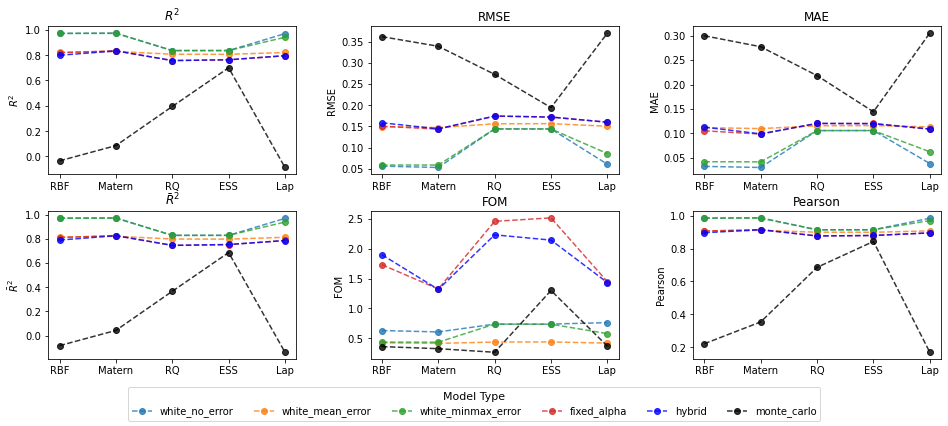
\includegraphics[width=\textwidth]{LatexPlots/CV_plots/metrics_compared.png}
    \caption{Comparison of the average performance of each model type and for each kernel across all 10 folds of the training/validation data for each metric. Note: The \texttt{combinedkernel} approach is excluded here for clarity, but is included in all subsequent evaluations.}
    \label{fig:broad_comparison}
\end{figure}
The average rank of each model across all metrics is shown in Table~\ref{tab:rankingtable}. The heatmap in Figure~\ref{fig:CV_sidebyside} (left) illustrates each model's ranking by metric. We can observe that the rankings are fairly consistent across metrics.
To examine this further we plot a dendrogram of their pairwise distances between metric ranking results in Figure~\ref{fig:CV_sidebyside} (middle). From this, we observe that the FOM produces noticeably different rankings compared to the other metrics. The most divergent metrics appear to be FOM, \(R^2\), and MAE.
To explore this further, we plot a scatter diagram in Figure~\ref{fig:CV_sidebyside}(right) with \(R^2\) on the x-axis, FOM on the y-axis, and MAE shown as the color scale. This highlights a clear group of the top 8 models, which form a distinctly optimal cluster. These are examined in more detail in the following section.
\begin{figure}[H]
    \centering
    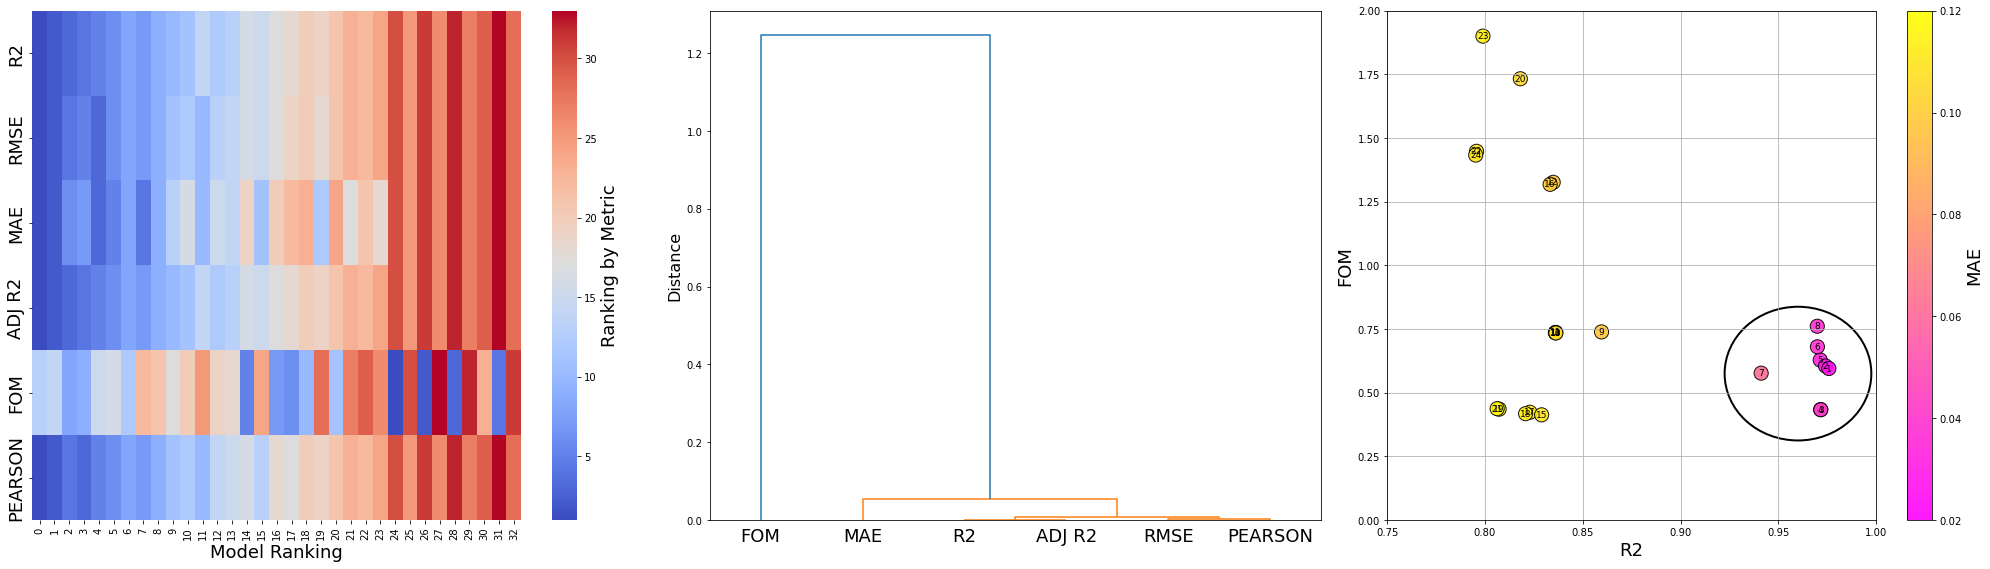
\includegraphics[width=\textwidth]{LatexPlots/CV_plots/ranking_visualisation.png}
    \caption{Left: Heatmap showing each model’s rank across the evaluation metrics. The x-axis lists models according to their ranking in Table~\ref{tab:rankingtable}, and the y-axis shows the metrics. The color bar represents rank (blue indicates better rank, red indicates worse). 
    Middle: Dendrogram showing hierarchical clustering of metrics based on how similarly they rank models. The vertical axis denotes correlation distance—smaller values indicate higher agreement between metric rankings.
    Right: Scatter plot of all models with \(R^2\) on the x-axis, FOM on the y-axis, and MAE represented by the color of each point. Models are indexed by their rank from Table~\ref{tab:rankingtable}.}
    \label{fig:CV_sidebyside}
\end{figure}



\subsubsection*{Training on 90\% of Data}
After identifying the top 8 models forming a high-performing cluster in Figure~\ref{fig:CV_sidebyside} (right),
 we retrained these models using the full 90\% of the data previously used for cross-validation. The optimized hyperparameters for these final models are detailed in Table~\ref{tab:final_gpr_hyperparams}. 
To evaluate generalization performance, we tested each model on the remaining 10\% of unseen data and visualized their results in Figure~\ref{fig:comparing_metrics}.
 The left panel shows a heatmap of model rankings across six metrics, and the right panel presents a scatter plot of $R^2$ vs FoM, with color indicating RMSE. 
 Model ranks are annotated in the scatter to highlight relative performance.
As shown, the rankings remain fairly consistent across metrics, with some variation in the FoM. The best performing models on the test set are \texttt{RBFMat}, \texttt{Matnoerr}, and \texttt{RBFnoerr} are ranked 1st, 2nd, and 3rd respectively.
These models achieve the strongest trade-offs between predictive accuracy and uncertainty calibration, making them the most promising candidates for deployment.
\begin{figure}[H]
    \centering
    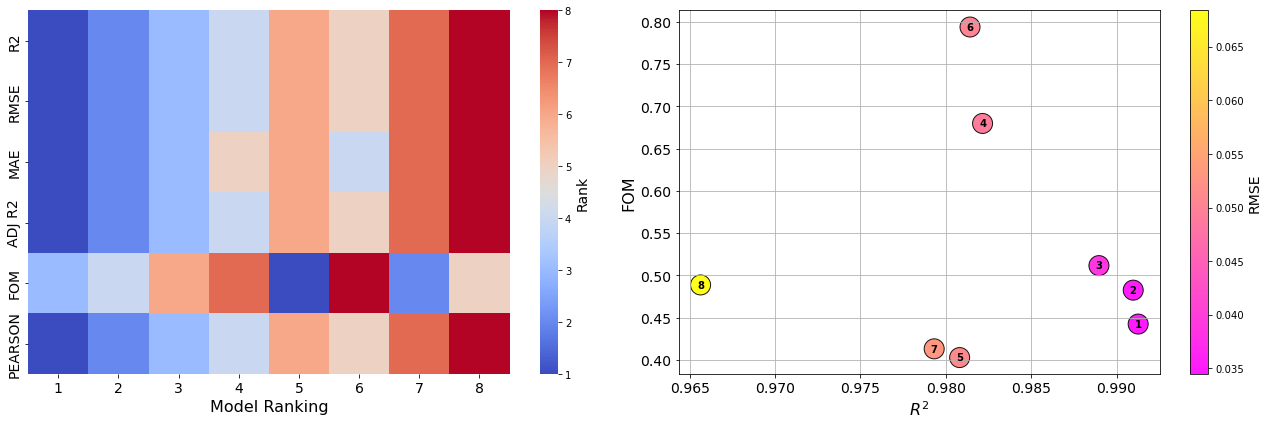
\includegraphics[width=\textwidth]{LatexPlots/final_gps_plots/metric_of_finalists_comparison.png}
    \caption{Left: Heatmap of top 8 model rankings by metric indexed by ranking.
    Right: Scatter of FOM against \(R^2\) with the colour bar representing the RMSE.
    The Rankings are given in Table~\ref{tab:finalmadelsrankingtable}.}
    \label{fig:comparing_metrics}
\end{figure}
From these visualizations, we observe that while all models perform well, they differ in how they handle local noise.
Let's examine the \texttt{RBFMat} model. It remains smooth where the data is clean but responds sharply in regions containing outliers or local irregularities.
This behaviour is reflected in its optimized hyperparameters (Table~\ref{tab:final_gpr_hyperparams}). The RBF component has long characteristic length scales (around 1.0--1.5) and a large scale factor ($2.34$),
which captures the global smooth structure of the data. Meanwhile, the Matern component has much shorter length scales (mostly $< 0.5$) and a smaller scale ($0.207$), allowing it to respond to local variability—effectively modeling input-dependent noise.
In contrast, models using a single kernel with a \texttt{WhiteKernel} for noise (e.g., \texttt{Mat\_noerr}, \texttt{RBF\_noerr}) appear smoother overall. These models result in smaller length scales and relatively small noise variances ($\sigma_n^2 < 0.01$).
When using tighter optimisation bounds for noise in the \texttt{min\_maxerr} models, we observe from Table~\ref{tab:final_gpr_hyperparams} that the noise hyperparameter consistently sits at or near the lower bound. 
This suggests that the GP is compensating for noise directly through the kernel, not through the explicit noise model. This provides further credibility to the \texttt{RBFMat} combined model, where the noise appears to be effectively captured within the \texttt{Matern} kernel.
Finally, examining Laplacian-based kernel models (\texttt{Laplace\_noerr} and \texttt{Laplace\_minmaxerr}), which only have a single hyperparameter ($\gamma$), they still perform reasonably well but tend to produce more linear predictions. This is likely due to their limited flexibility compared to other kernels.
Based on our metrics calculated and visualised in Figure~\ref{fig:comparing_metrics} and our qualitative examination of the crosscuts in Figure~\ref{fig:crosscuts_bestmodels}, we conclude that the \texttt{RBFMat} model offers the best trade-off between flexibility, interpretability, and robustness.
However, since the \texttt{RBFMat} combined kernel model optimises 10 hyperparameters, there is a risk we are overfitting to the data. Therefore, we retain the \texttt{Mat\_noerr} model for comparative purposes, as it offers a smooth fit with fewer hyperparameters.

\begin{figure}[H]
    \centering
    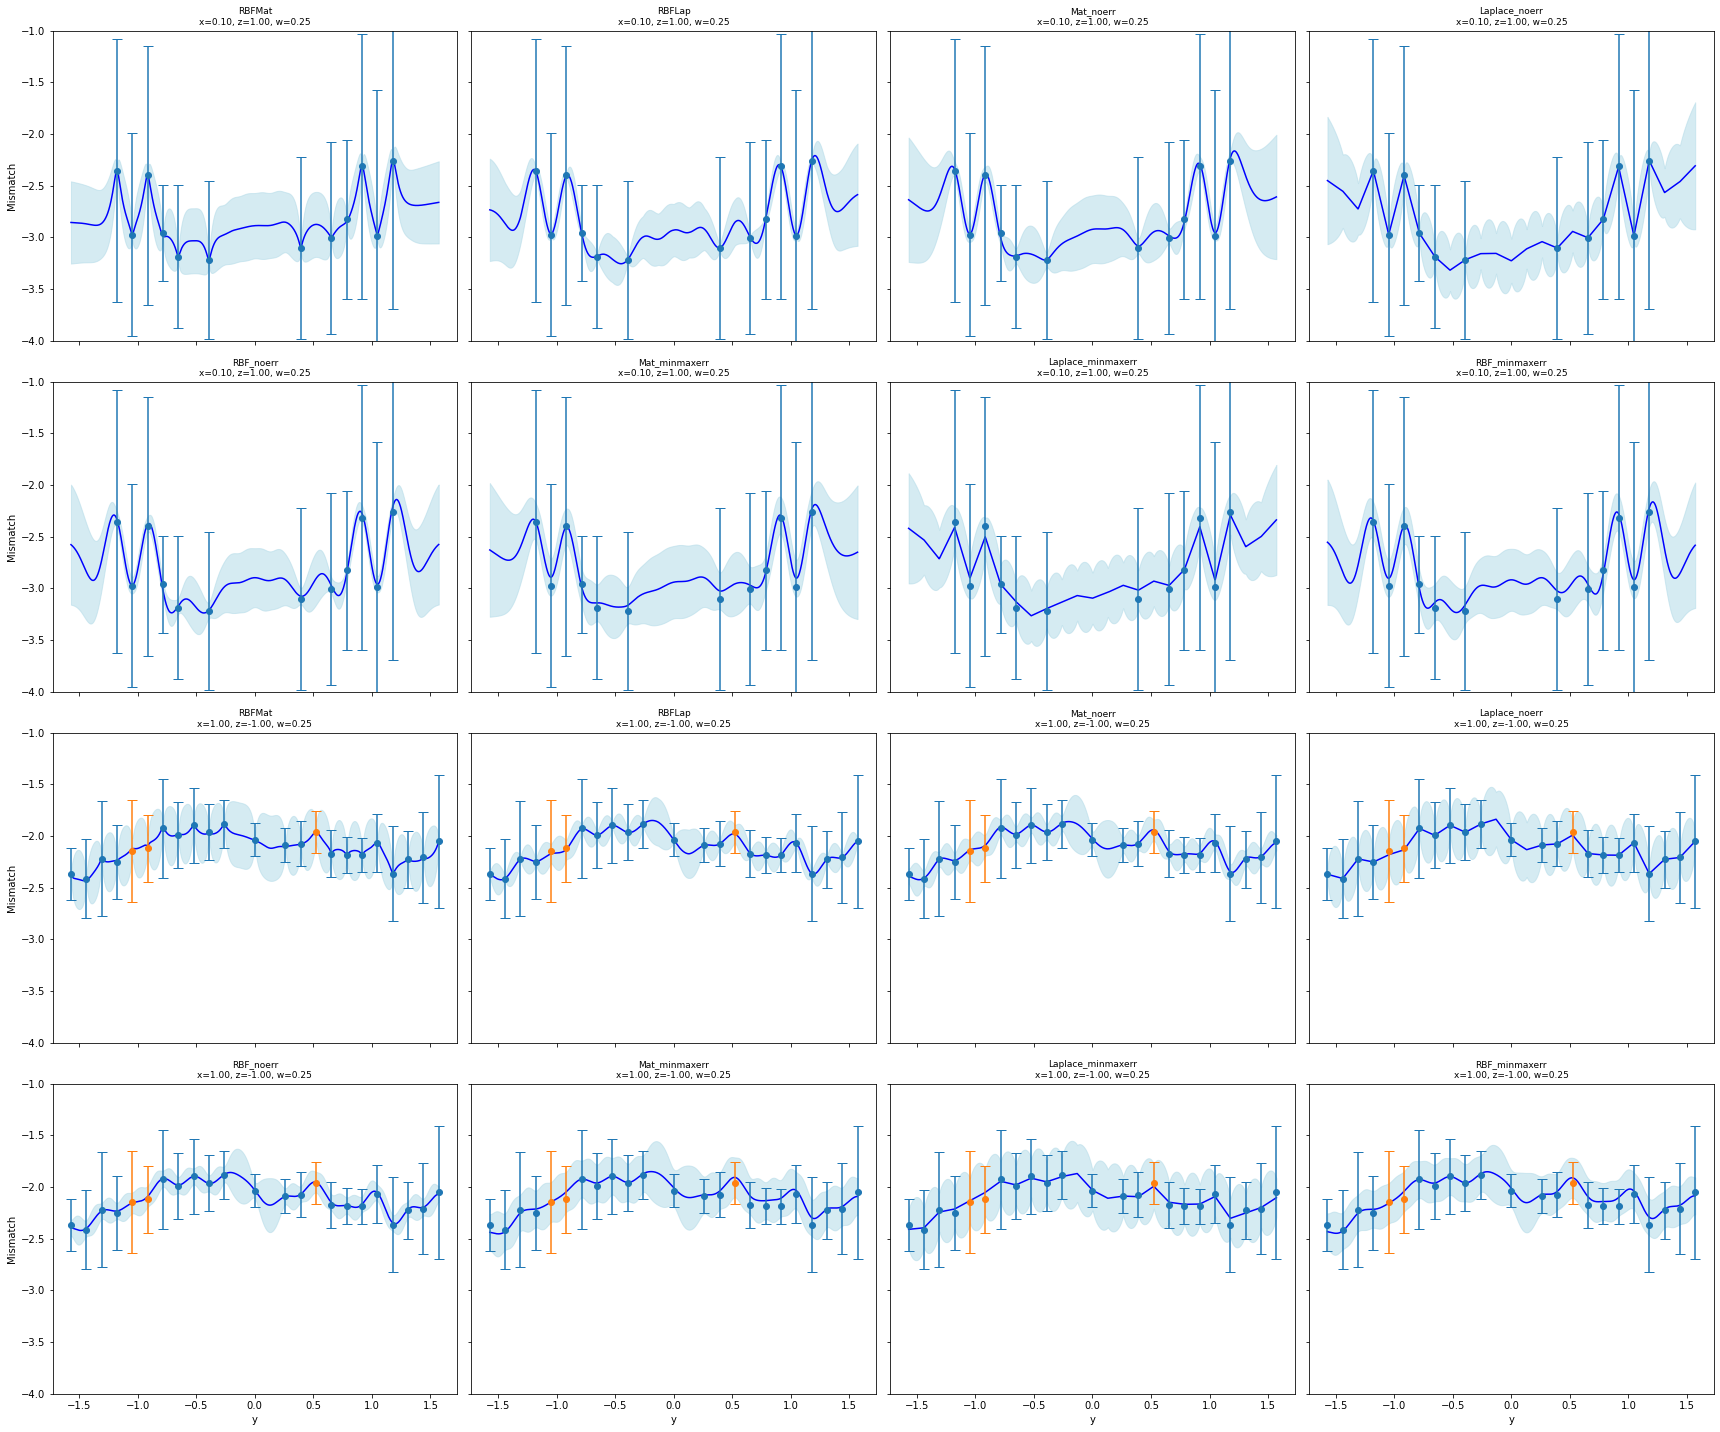
\includegraphics[width=1\textwidth]{LatexPlots/final_gps_plots/gps_crosscuts_bestmodels.png}
    \caption{Comparing Cross-cuts of best models. See text for details. Recall that $z=1\ (z=-1)$ corresponds
    to mass ratio of $q=1\ (q=1/4)$, and similarly $w=0.25$ corresponds to $M_\text{tot}=37.5M_\odot$.}
    \label{fig:crosscuts_bestmodels}
\end{figure}

\begin{table}[H]
\centering
\caption{\todo{Explain what scale 1/2 mean} Optimized Hyperparameters for Final GPR Models}
\footnotesize  % Smaller than normalsize, slightly larger than scriptsize
\renewcommand{\arraystretch}{1.15}  % Slightly tighter row spacing
\setlength{\tabcolsep}{4pt}  % Reduce column padding
\label{tab:final_gpr_hyperparams}
{\fontsize{7}{9.5}\selectfont
\begin{tabular}{|c|c|c|c|c|c|c|}
\hline
\textbf{Model} & \textbf{Kernel 1} & \textbf{Scale 1} & \textbf{Length Scales 1} & \textbf{Kernel 2} & \textbf{Scale 2} & \textbf{Length Scales 2 / Noise} \\
\hline
\texttt{RBFMat} & RBF & $2.34$ & $[1.00, 1.51, 1.38, 1.36]$ & Matern ($\nu = 0.75$) & $0.207$ & $[0.0996, 0.0582, 0.414, 2.31]$ \\
\texttt{RBFLap} & RBF & $0.354$ & $[0.10, 0.10, 1.18, 2.91]$ & Laplacian ($\gamma = 0.964$) & $0.292$ & --- \\
\texttt{Mat\_noerr} & Matern ($\nu = 1.75$) & $0.926$ & $[0.227, 0.20, 1.15, 2.85]$ & White & --- & $\sigma_n^2 = 0.00637$ \\
\texttt{Laplace\_noerr} & Laplacian ($\gamma = 0.358$) & $7.24$ & --- & White & --- & $\sigma_n^2 = 10^{-6}$ \\
\texttt{RBF\_noerr} & RBF & $0.728$ & $[0.112, 0.112, 0.958, 1.6]$ & White & --- & $\sigma_n^2 = 0.00728$ \\
\texttt{Mat\_minmaxerr} & Matern ($\nu = 1.75$) & $1.14$ & $[0.27, 0.22, 1.34, 4.73]$ & White & --- & $\sigma_n^2 = 0.0439$ \\
\texttt{Laplace\_minmaxerr} & Laplacian ($\gamma = 0.284$) & $6.60$ & --- & White & --- & $\sigma_n^2 = 0.0439$ \\
\texttt{RBF\_minmaxerr} & RBF & $0.821$ & $[0.12, 0.115, 1.19, 2.52]$ & White & --- & $\sigma_n^2 = 0.0439$ \\
\hline
\end{tabular}}
\end{table}


\subsubsection*{MCMC}
\textbf{MCMC on \texttt{RBFMatern}}
\begin{figure}[H]
    \centering
    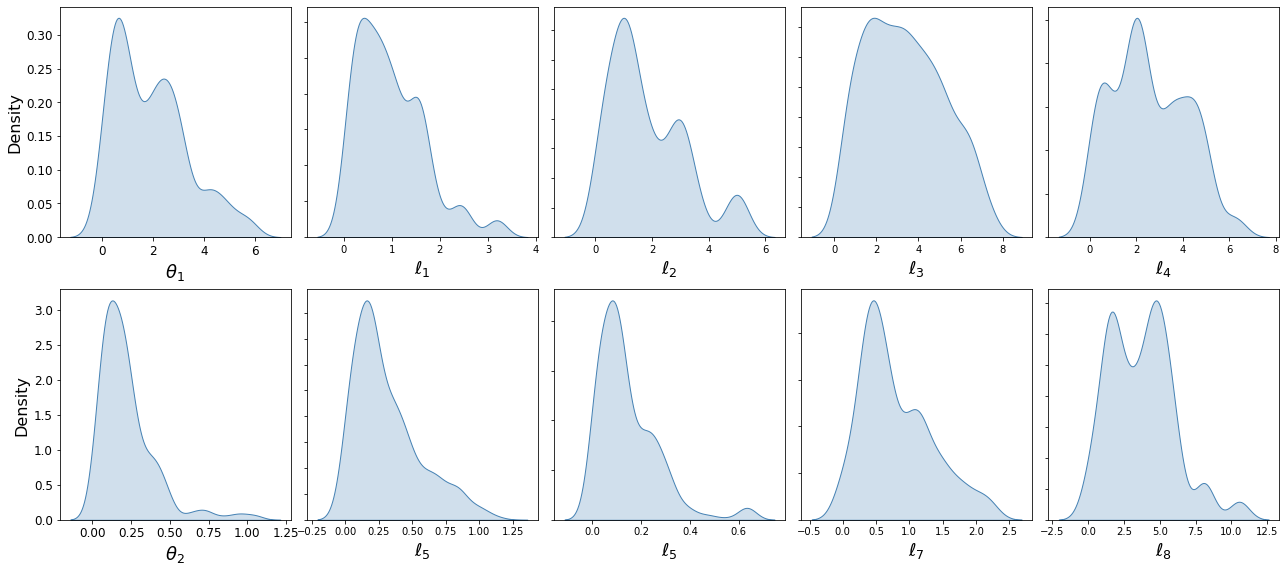
\includegraphics[width=1\textwidth]{LatexPlots/final_gps_plots/MCMCRBFMat.png}
    \caption{MCMC on \texttt{RBFMatern} combined kernel model}
    \label{fig:MCMCRBFMatern}
\end{figure}

\textbf{MCMC on \texttt{Maternnoerr}}
\begin{figure}[H]
    \centering
    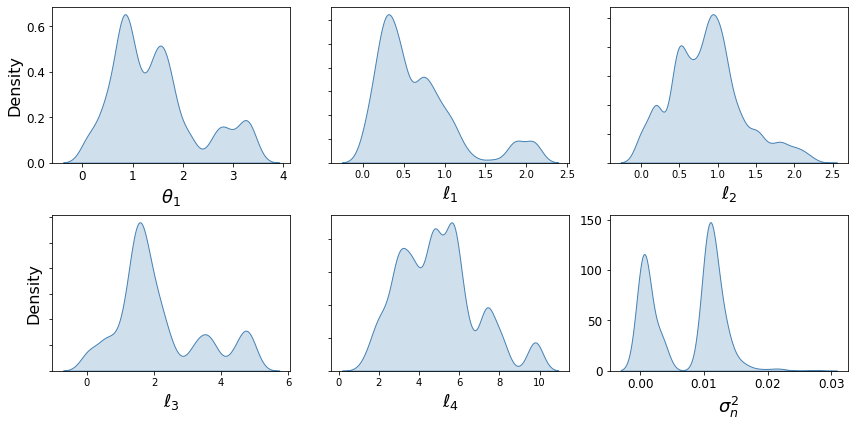
\includegraphics[width=1\textwidth]{LatexPlots/final_gps_plots/MCMCWhiteMat.png}
    \caption{MCMC on \texttt{Maternoerr} model}
    \label{fig:MCMCMaternnoerr}
\end{figure}


\section{Conclusion}
\begin{itemize}
    \item successfully developed accurate models
    \item Evaluated a wide variety of kernels
    \item Used MCMC to visuale hyper-parameters posteriors
    \item Compared 4d to 7d model how did reducing the parameters space effect the model, loose much information??
    \item Potential Scaling issues
\end{itemize}


\section{Discussion}
\begin{itemize}
    \item In future would like to build a model with kernel uncertainty built into model, full gpr
    \todo{Add the 7D discussion here}
    \item Combined GPR , including multiple posteriors weighted
    \item Use other GPR methods, sparse GPR \Sean{(read and bried comment)}
    \item Maybe using physical constraints somewhat in the model
\end{itemize}

\appendix

\section{Appendix A: Derivation of Predictive Distribution}
\label{appendix:A}
Using Bayes' Theorem applied to continuous probabilities, we have:
\[
p(f_* | f) = \frac{p(f_*, f)}{p(f)}.
\]
we have:
$$p(f_*,f) = \frac{1}{2\pi\sqrt{\mathbf{|C|}}}\exp \left(-\frac{1}{2} 
\begin{bmatrix} f \\ f_*  \end{bmatrix}^T\mathbf{C^{-1}}\begin{bmatrix} f  \\ f_* \end{bmatrix}\right)$$
and 
\[
p(f) = \frac{1}{\sqrt{2\pi} |K|^{1/2}}
\exp \left(-\frac{1}{2} f^T K^{-1} f \right).
\]

\noindent
\textbf{Legend}
\begin{itemize}
    \item \textbf{Covariance matrices:}
    \begin{itemize}
        \item \( K = K(X, X) \): Covariance matrix of the training inputs.
        \item \( K_{**} = K(X_*, X_*) \): Covariance matrix of the test inputs.
        \item \( K_* = K(X, X_*) = K(X_*, X)^\top \): Cross-covariance between training and test inputs.
    \end{itemize}
    
    \item \textbf{Joint covariance matrix:}
    \[
    C = \begin{bmatrix}
    K & K_* \\
    K_*^\top & K_{**}
    \end{bmatrix}
    \]
    
    \item \textbf{Determinant of \( \mathbf{C} \):}
    \[
    |\mathbf{C}| = K K_{**} - K_* K_*^\top
    \]
    
    \item \textbf{Inverse of \( \mathbf{C} \):}
    \[
    \mathbf{C}^{-1} = \frac{1}{|\mathbf{C}|}
    \begin{bmatrix}
    K_{**} & -K_* \\
    -K_*^\top & K
    \end{bmatrix}
    \]
    
    \item \textbf{Mean functions:}
    \[
    m(X) = m(X_*) = 0
    \]
\end{itemize}



\section{Appendix B: Kernel Formulas}
\label{appendix:B}
\subsubsection*{Radial Basis Function (RBF) Kernel}
\[
k(x, x') = \sigma_f^2 \exp\left( -\frac{(x - x')^2}{2\ell^2} \right)
\]
This kernel assumes smooth and infinitely differentiable functions, modeling local variations.


\subsubsection*{Rational Quadratic Kernel}
\[
k(x, x') = \sigma_f^2 \left( 1 + \frac{(x - x')^2}{2 \alpha \ell^2} \right)^{-\alpha}
\]
This kernel can be seen as a scale mixture of RBF kernels, allowing for multi-scale behavior.


\subsubsection*{Periodic Kernel}
\[
k(x, x') = \sigma_f^2 \exp\left( -\frac{2}{\ell^2} \sin^2\left( \frac{\pi (x - x')}{p} \right) \right)
\]
This kernel models repeating structures with period \( p \).

\subsubsection*{Matern Kernel}
\[
k(x, x') = \sigma_f^2 \frac{2^{1-\nu}}{\Gamma(\nu)} \left( \frac{\sqrt{2\nu} |x - x'|}{\ell} \right)^\nu K_\nu\left( \frac{\sqrt{2\nu} |x - x'|}{\ell} \right)
\]
The Matern kernel allows for controlling the smoothness of functions via the parameter \( \nu \).


\subsubsection*{Laplace (Exponential) Kernel}
\[
k(x, x') = \sigma_f^2 \exp\left( -\gamma |x - x'| \right)
\]
Equivalent to the Matern kernel with \( \nu = \frac{1}{2} \), this kernel models rougher functions.


\subsubsection*{Linear (Dot-Product) Kernel}
\[
k(x, x') = \sigma_b^2 + x^\top x'
\]
This kernel grows with the similarity (inner product) between inputs, and it allows the function to vary globally. Since it depends directly on the values of \( x \) and \( x' \), not just their difference, it is non-stationary. It is particularly useful for modeling linear trends.


\section{Appendix C: Graphs of 4d finalist GPs}
\label{appendix:C}


\begin{figure}[H]
    \centering
    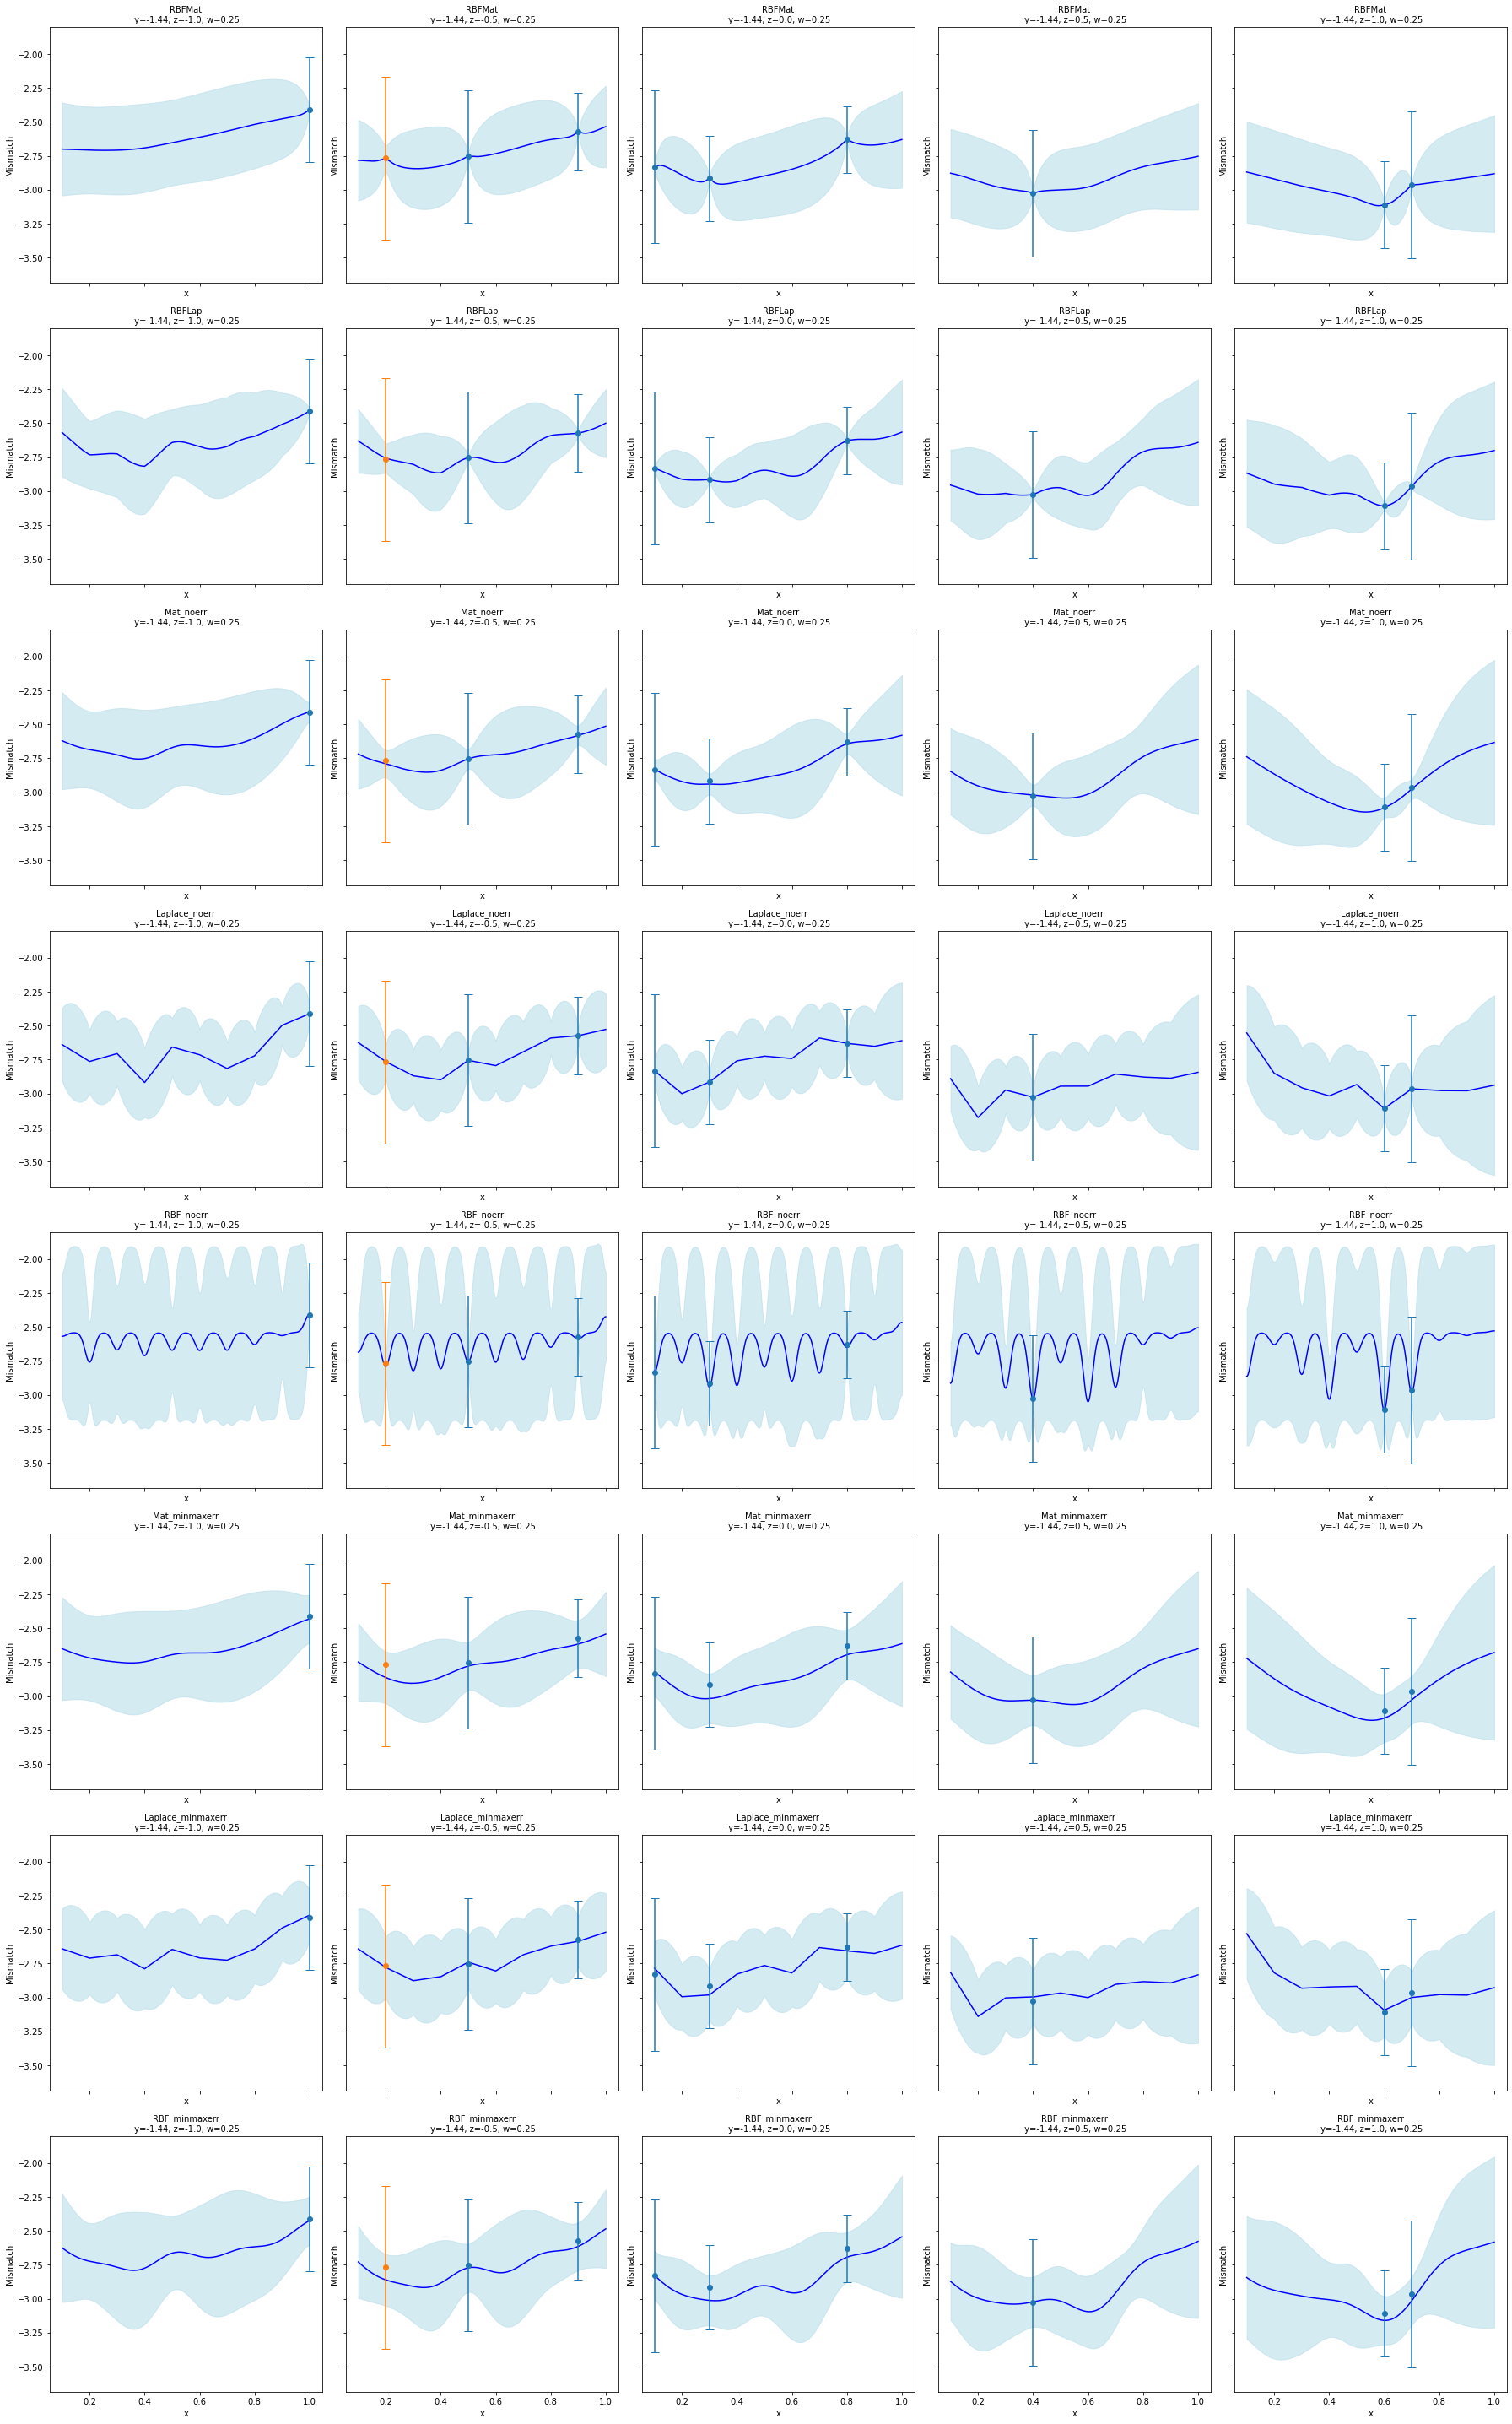
\includegraphics[width=0.8\textwidth]{LatexPlots/final_gps_plots/final_gps_ycuts.png}
    \caption{\todo{Improve caption} All 8 gps with cutting their y-axis}
    \label{fig:best8_ycuts}
\end{figure}


\begin{figure}[H]
    \centering
    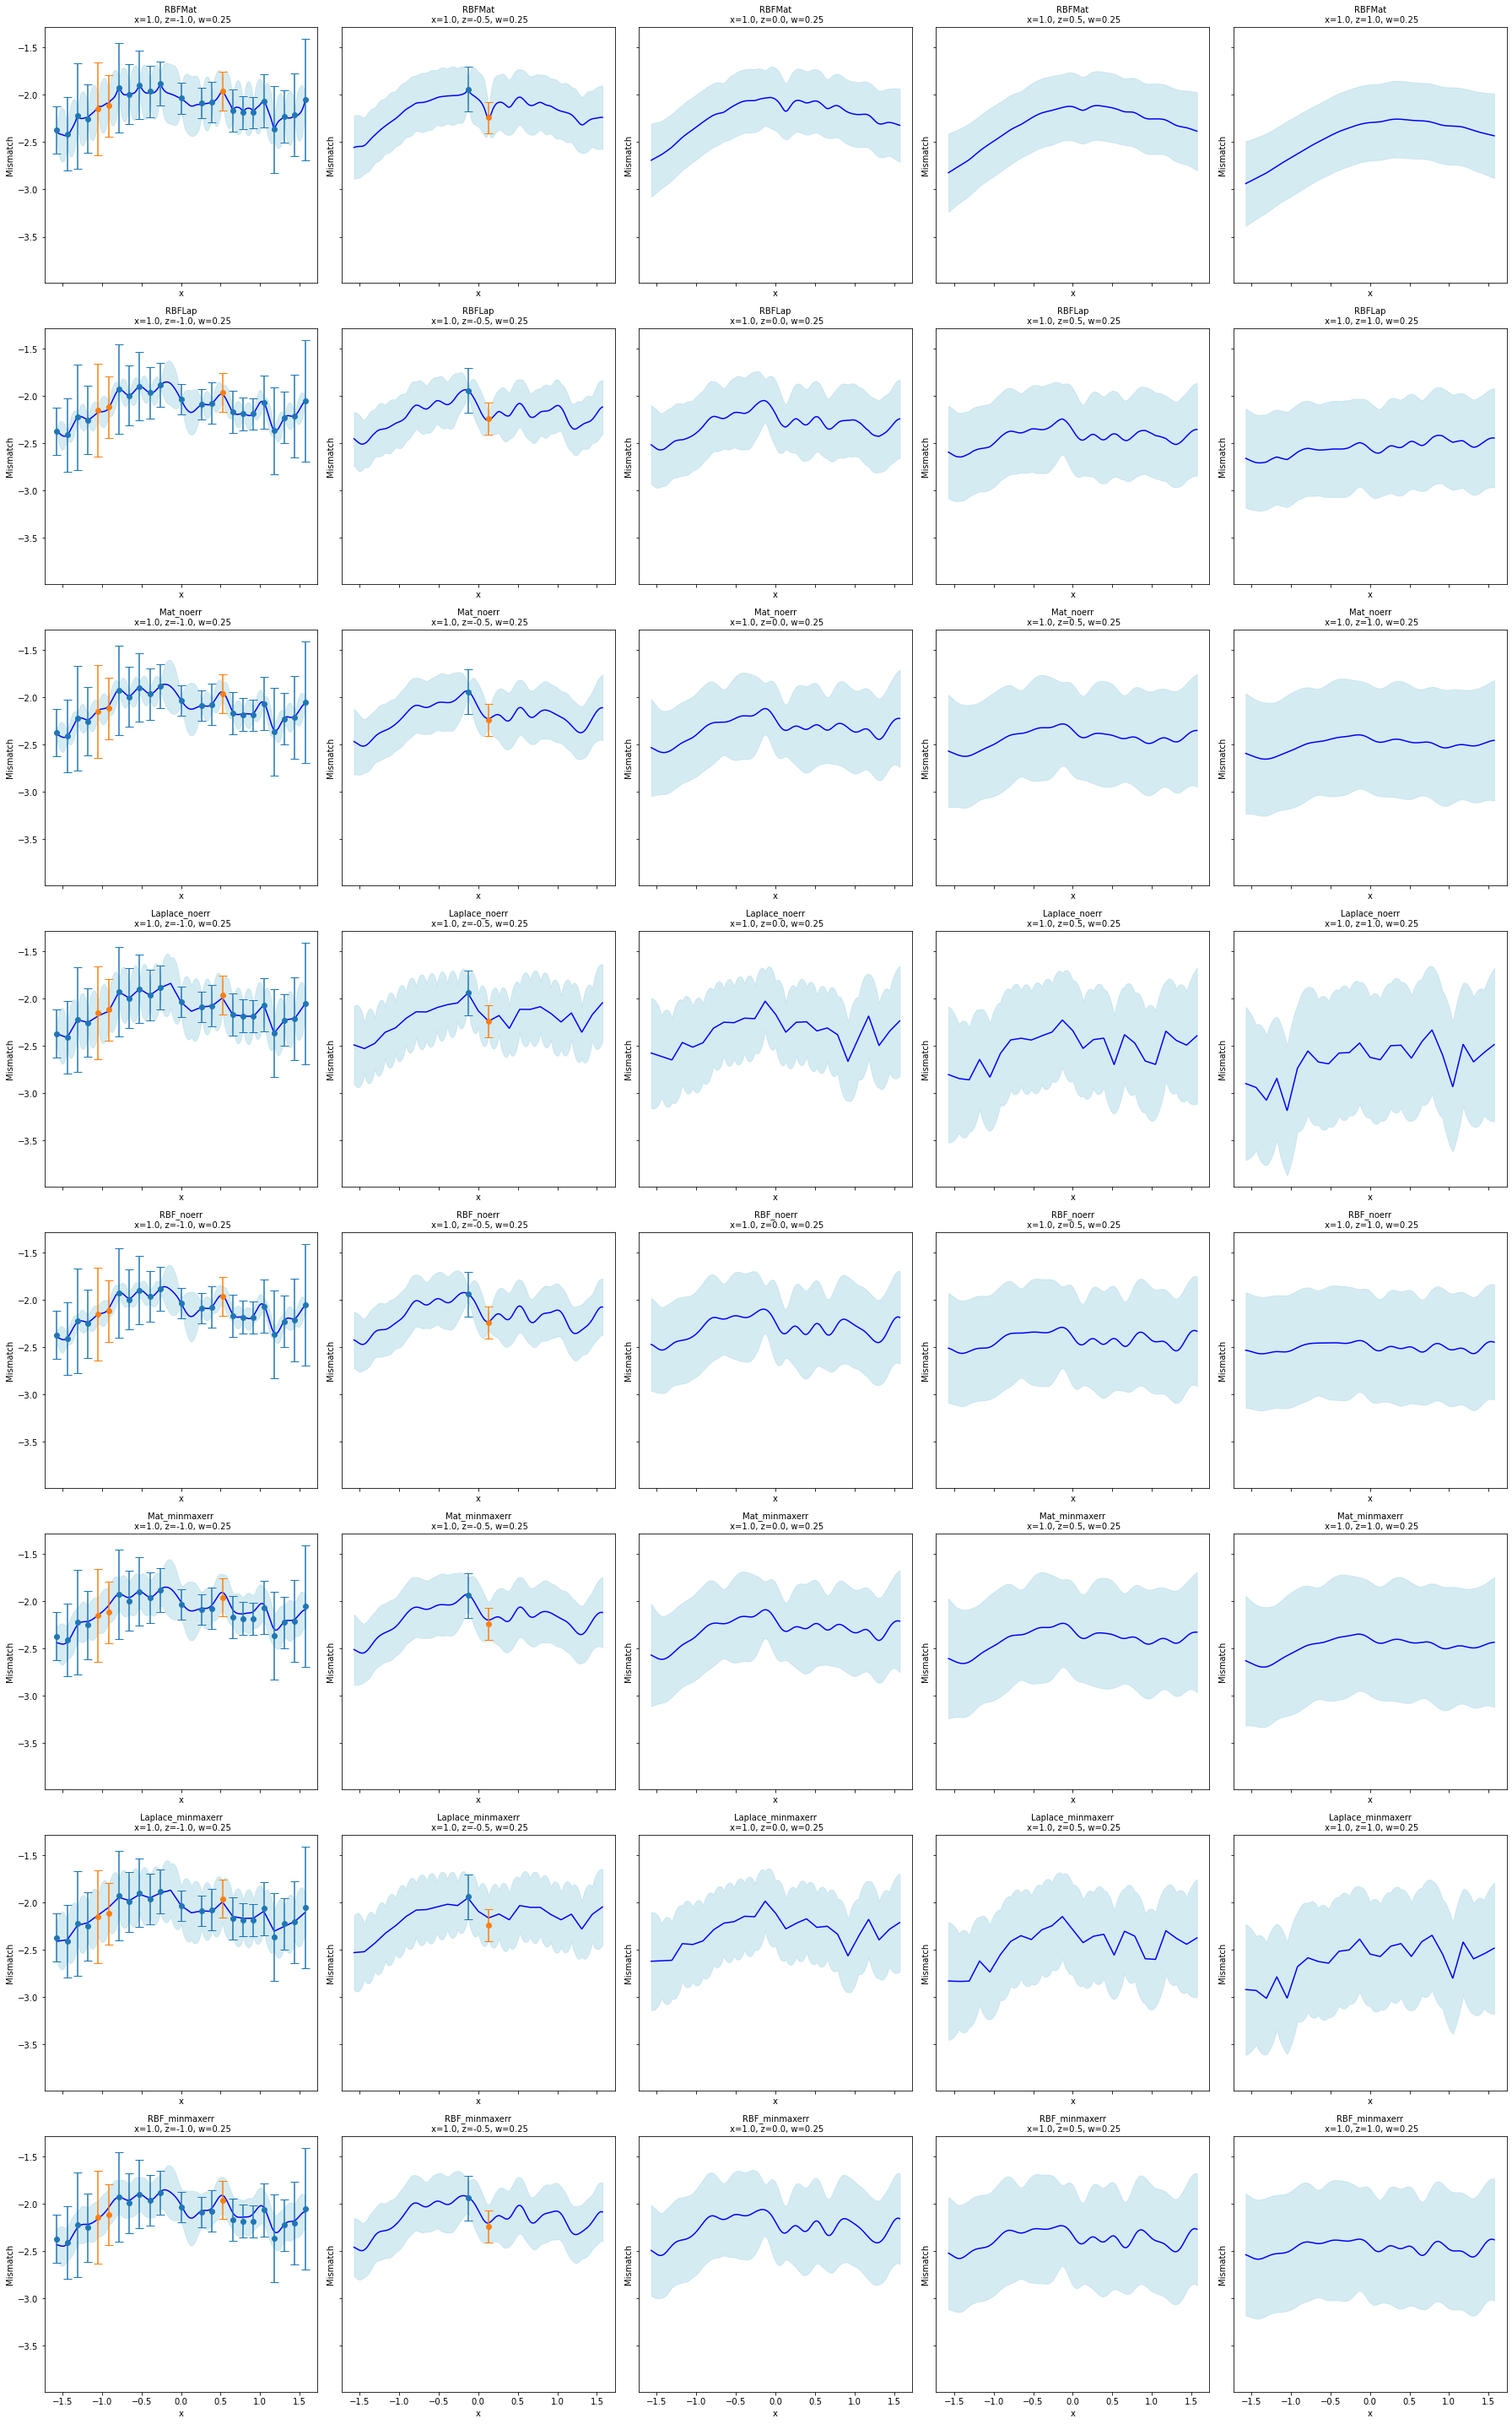
\includegraphics[width=0.8\textwidth]{LatexPlots/final_gps_plots/final_gps_xcuts.png}
    \caption{All 8 gps with cutting their x-axis}
    \label{fig:best8_xcuts}
\end{figure}

\begin{figure}[H]
    \centering
    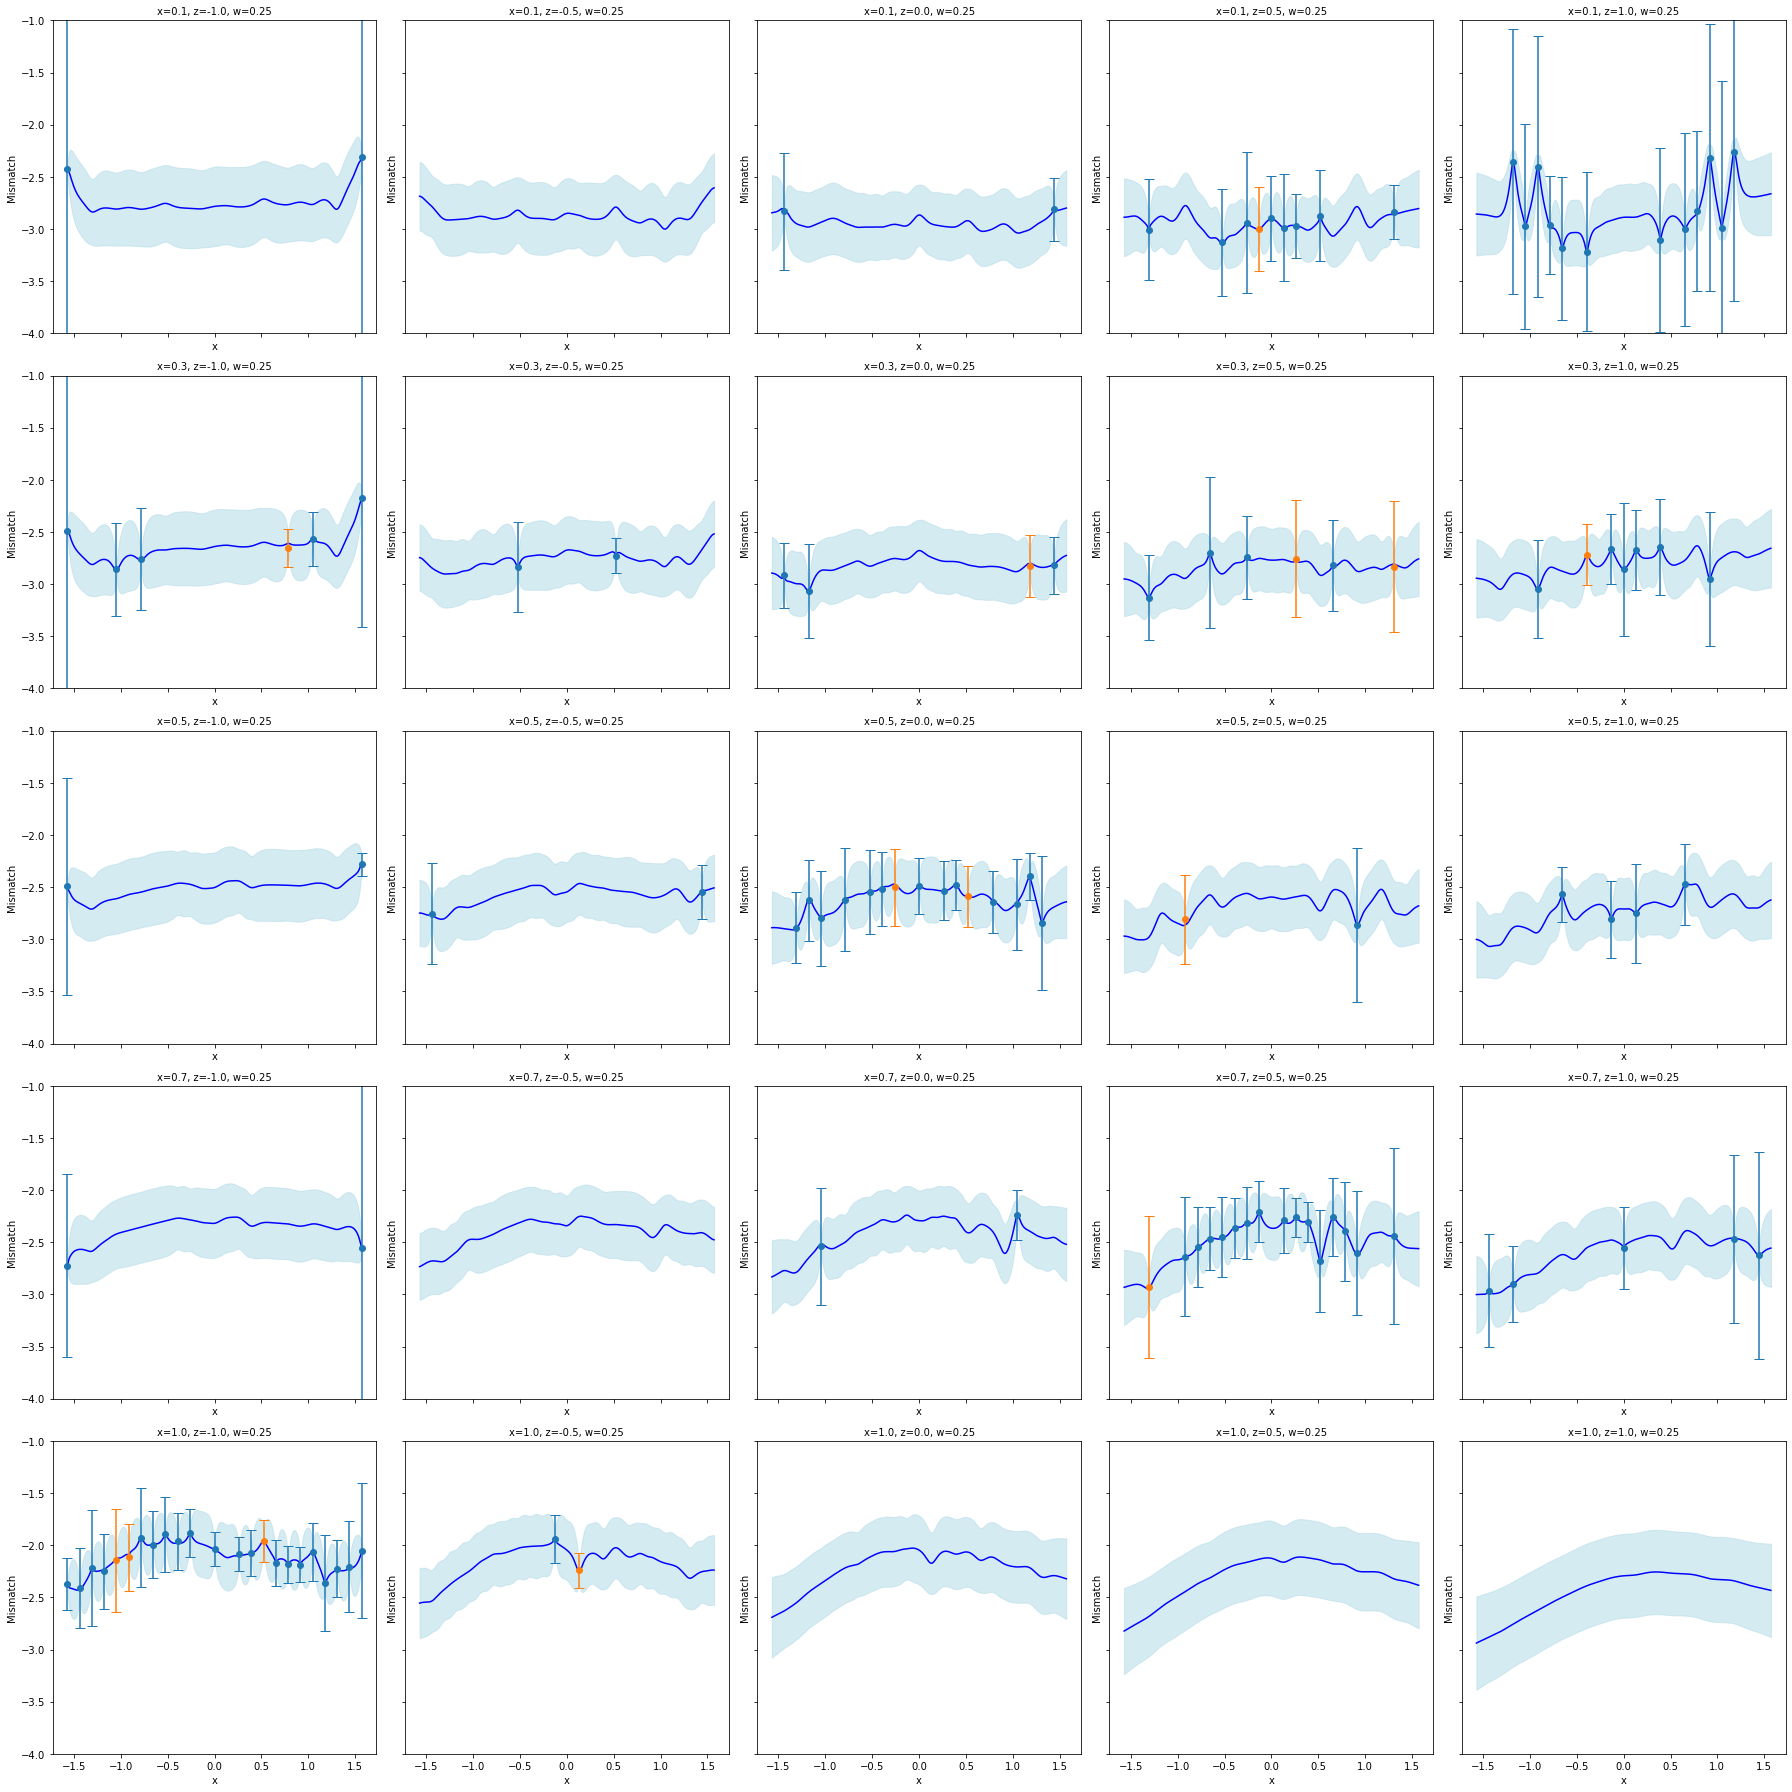
\includegraphics[width=0.8\textwidth]{LatexPlots/final_gps_plots/gps_rbfmatern_xcuts.png}
    \caption{Examining my chosen model RBF Matern kernel}
    \label{fig:RBF_Matern_xcuts}
\end{figure}


\section{Appendix D: Model Evaluation Table and graphs}
\label{appendix:D}

\begin{figure}[H]
    \centering
    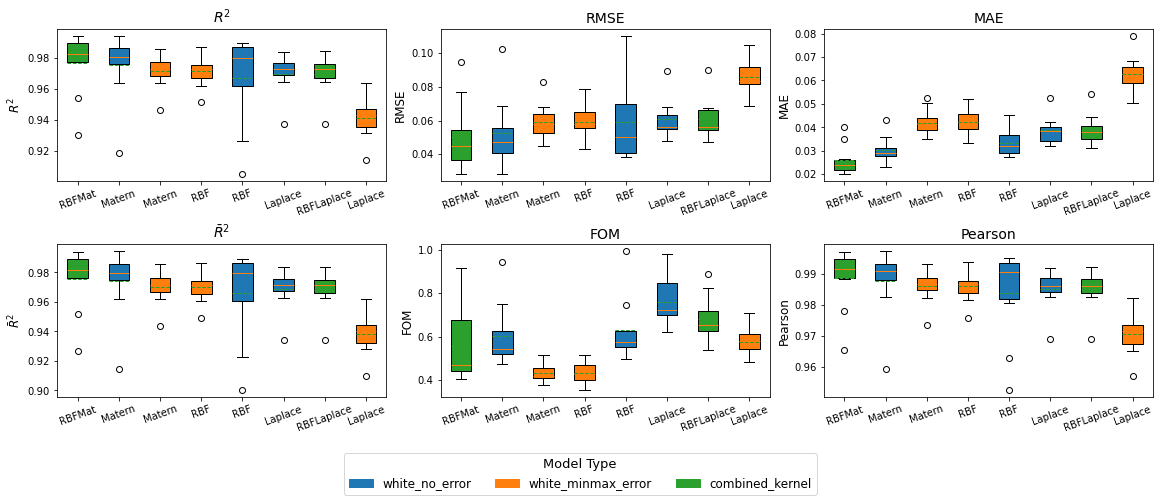
\includegraphics[width=0.8\textwidth]{LatexPlots/CV_plots/boxplots.png}
    \caption{Seeing how the best models performed over different clusters}
    \label{fig:boxplots}
\end{figure}

\begin{table}[H]
    \centering
    \caption{Final Model Rankings after training on 90\% and testing on 10\%}
    {\fontsize{7}{9.5}\selectfont
    \csvautotabular{LatexPlots/CV_plots/final_model_rankings.csv}}
    \label{tab:finalmadelsrankingtable}
\end{table}



\begin{table}[H]
    \centering
    \caption{All 32 Model Rankings from CV}
    {\fontsize{7}{9.5}\selectfont
    \csvautotabular{LatexPlots/CV_plots/model_rankings.csv}
    }
    \label{tab:rankingtable}
\end{table}
    

\section{Appendix E: Bin}
\label{appendix:bin}
\Sean{Moving Evaluation Metrics to Methods}

In figure \ref{tab:metrics-comparison}, we made a graphical representation of four out of six metrics used to evaluate our model’s accuracy. \cite{bible} discusses how these metrics provide a balanced assessment of model performance.
The Root Mean Squared Error (RMSE) and Mean Absolute Error (MAE) measure the average deviation of predictions from the true values, with RMSE penalizing larger errors more heavily.
The coefficient of determination \( R^2 \) quantifies how well the model predicts relative to the mean of the test set. It is computed as \( 1 \) minus the ratio of the squared residuals to the total variance. A value closer to \( 1 \) indicates better predictive performance.
The adjusted \( R^2 \) (\(\bar{R}^2\)) accounts for model complexity by penalizing excessive predictor variables, preventing overfitting.
The Figure of Merit (FOM) evaluates the ratio of a point’s prediction error to its associated standard deviation. A FOM near \( 1 \) is ideal, indicating that the model’s uncertainty estimates are well-calibrated. A FOM \( \ll 1 \) suggests an overly conservative model with large uncertainty, while a FOM \( \gg 1 \) may indicate overconfidence, failing to capture true variability.
The Pearson correlation coefficient measures the linear relationship between predictions and true values. A correlation of \( 1 \) (\(-1\)) signifies a perfect positive (negative) linear relationship, whereas a correlation of \( 0 \) indicates no linear association.



\begin{table}[H]
    \centering
    \renewcommand{\arraystretch}{4} % Adjust row spacing
    \setlength{\tabcolsep}{2pt} % Adjust column spacing
    \small % Reduce text size

    \begin{tabular}{|>{\centering\arraybackslash}m{2.5cm}|*{4}{>{\centering\arraybackslash}m{3cm}|}} 
        \hline
        \textbf{Metric Name} & \textbf{RMSE} & \textbf{\(R^2\)} & \textbf{FOM} & \textbf{Pearson Coefficient} \\ 
        \hline
        \textbf{Formula} & 
        \( \sqrt{\frac{1}{N} \sum (y_i - \hat{y}_i)^2} \)   & 
        \( 1 - \frac{\sum (y_i - \hat{y}_i)^2}{\sum (y_i - \bar{y})^2} \) &    
        \( \frac{RMSE}{\sigma} \) &  
        \( \frac{\text{cov}(y - \hat{y})}{\sigma_y \sigma_{\hat{y}}} \) \\ 
        \hline
        \textbf{Visual Illustration} &  
        \adjustbox{valign=c}{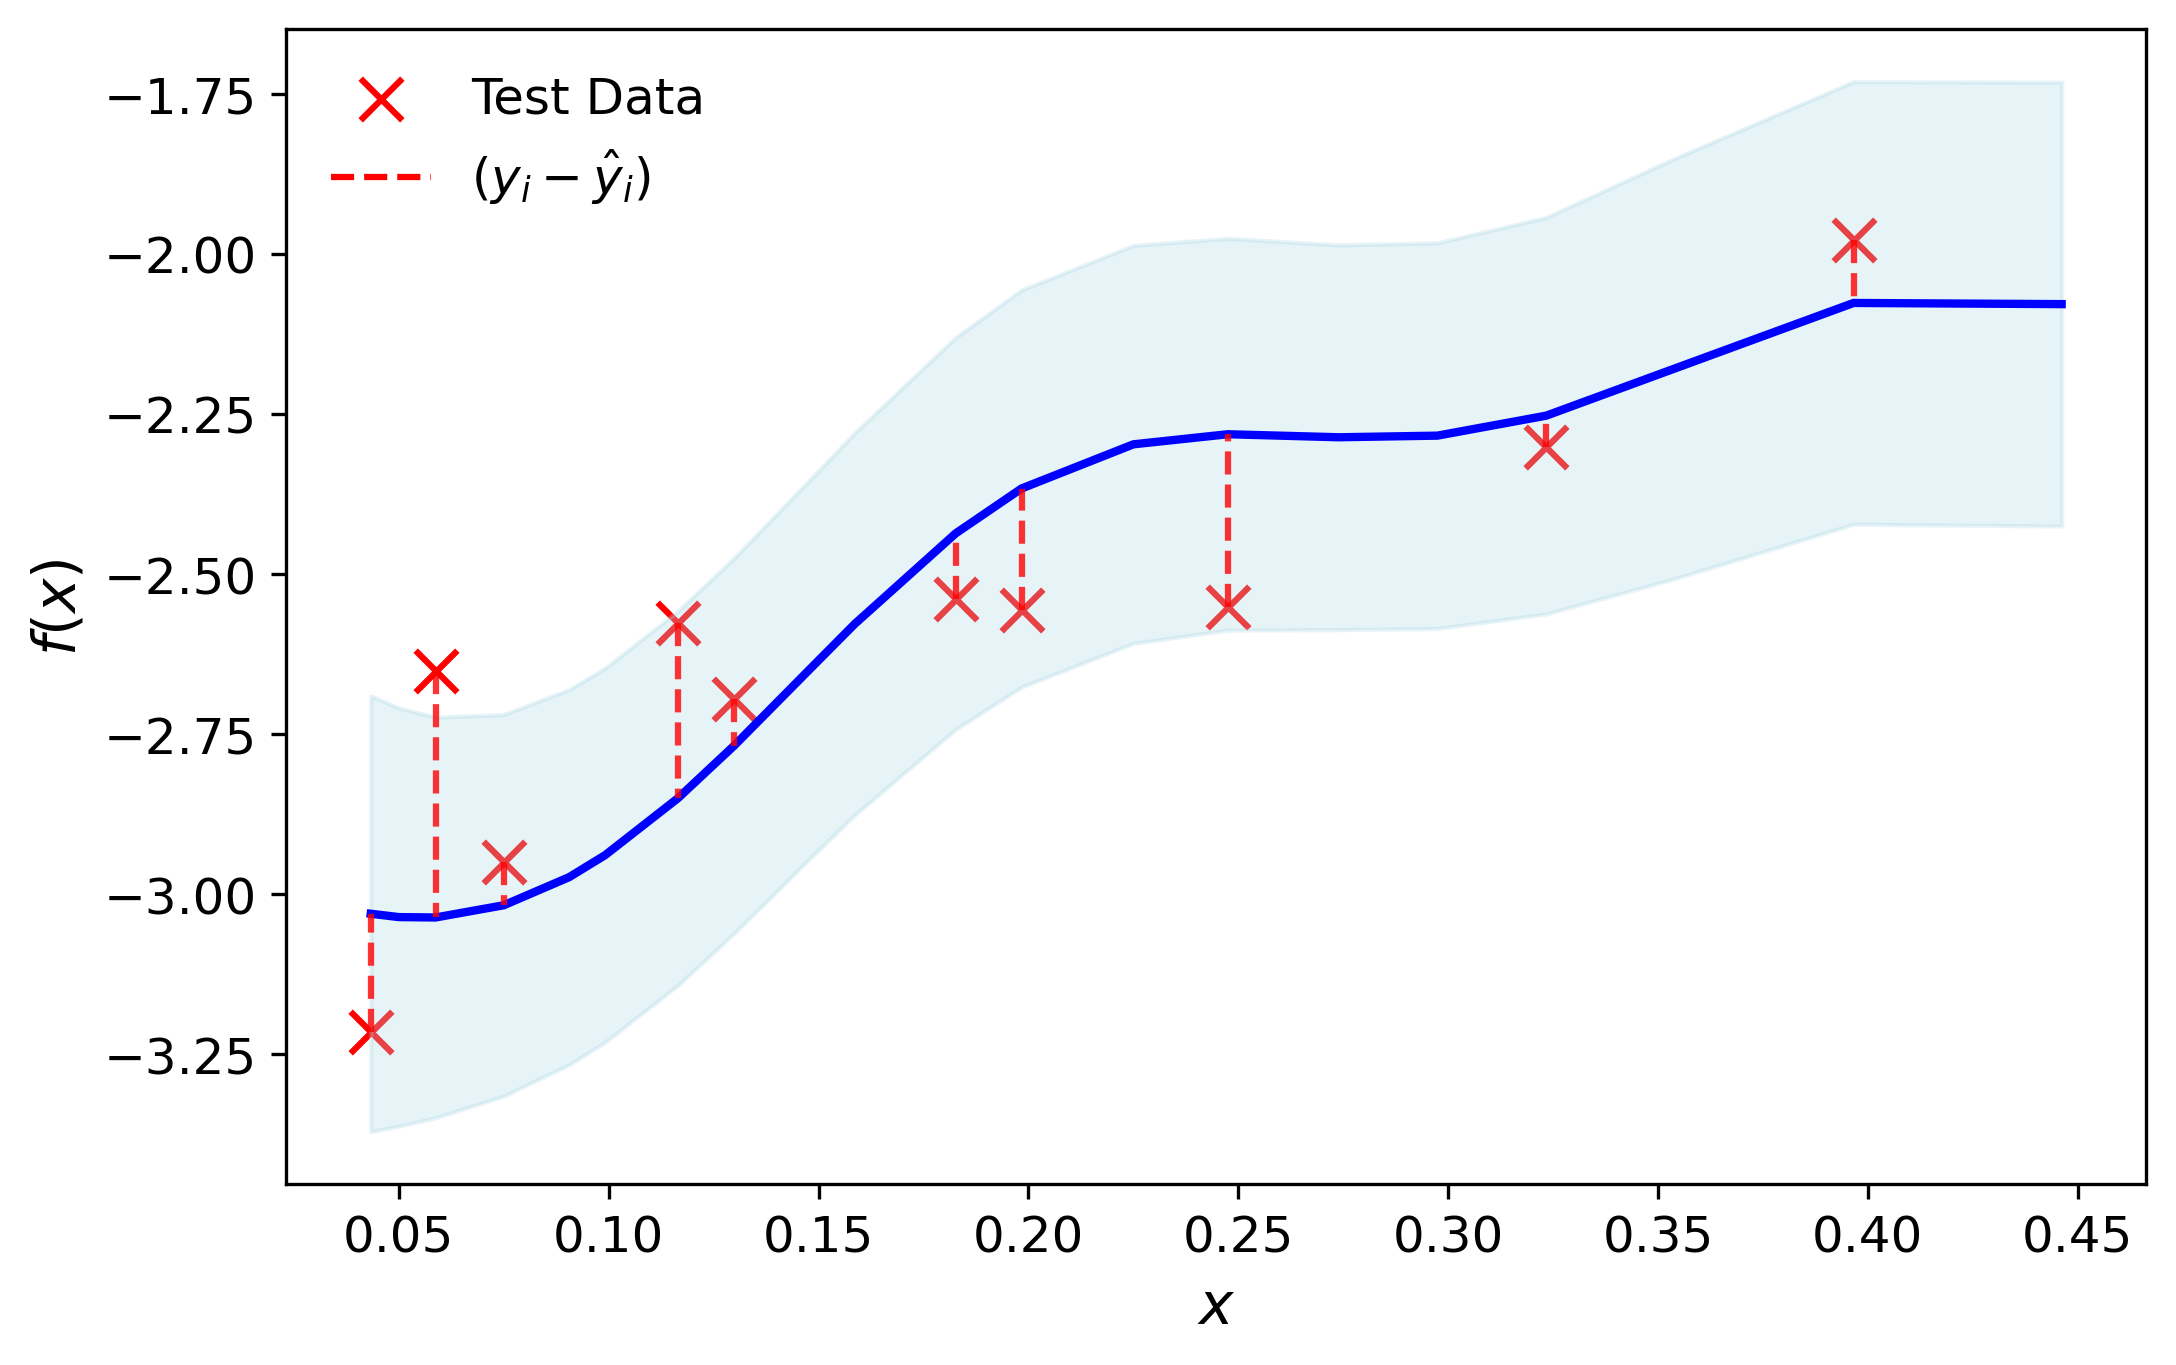
\includegraphics[width=3cm]{LatexPlots/1dplots/MAE.png}} &  
        \adjustbox{valign=c}{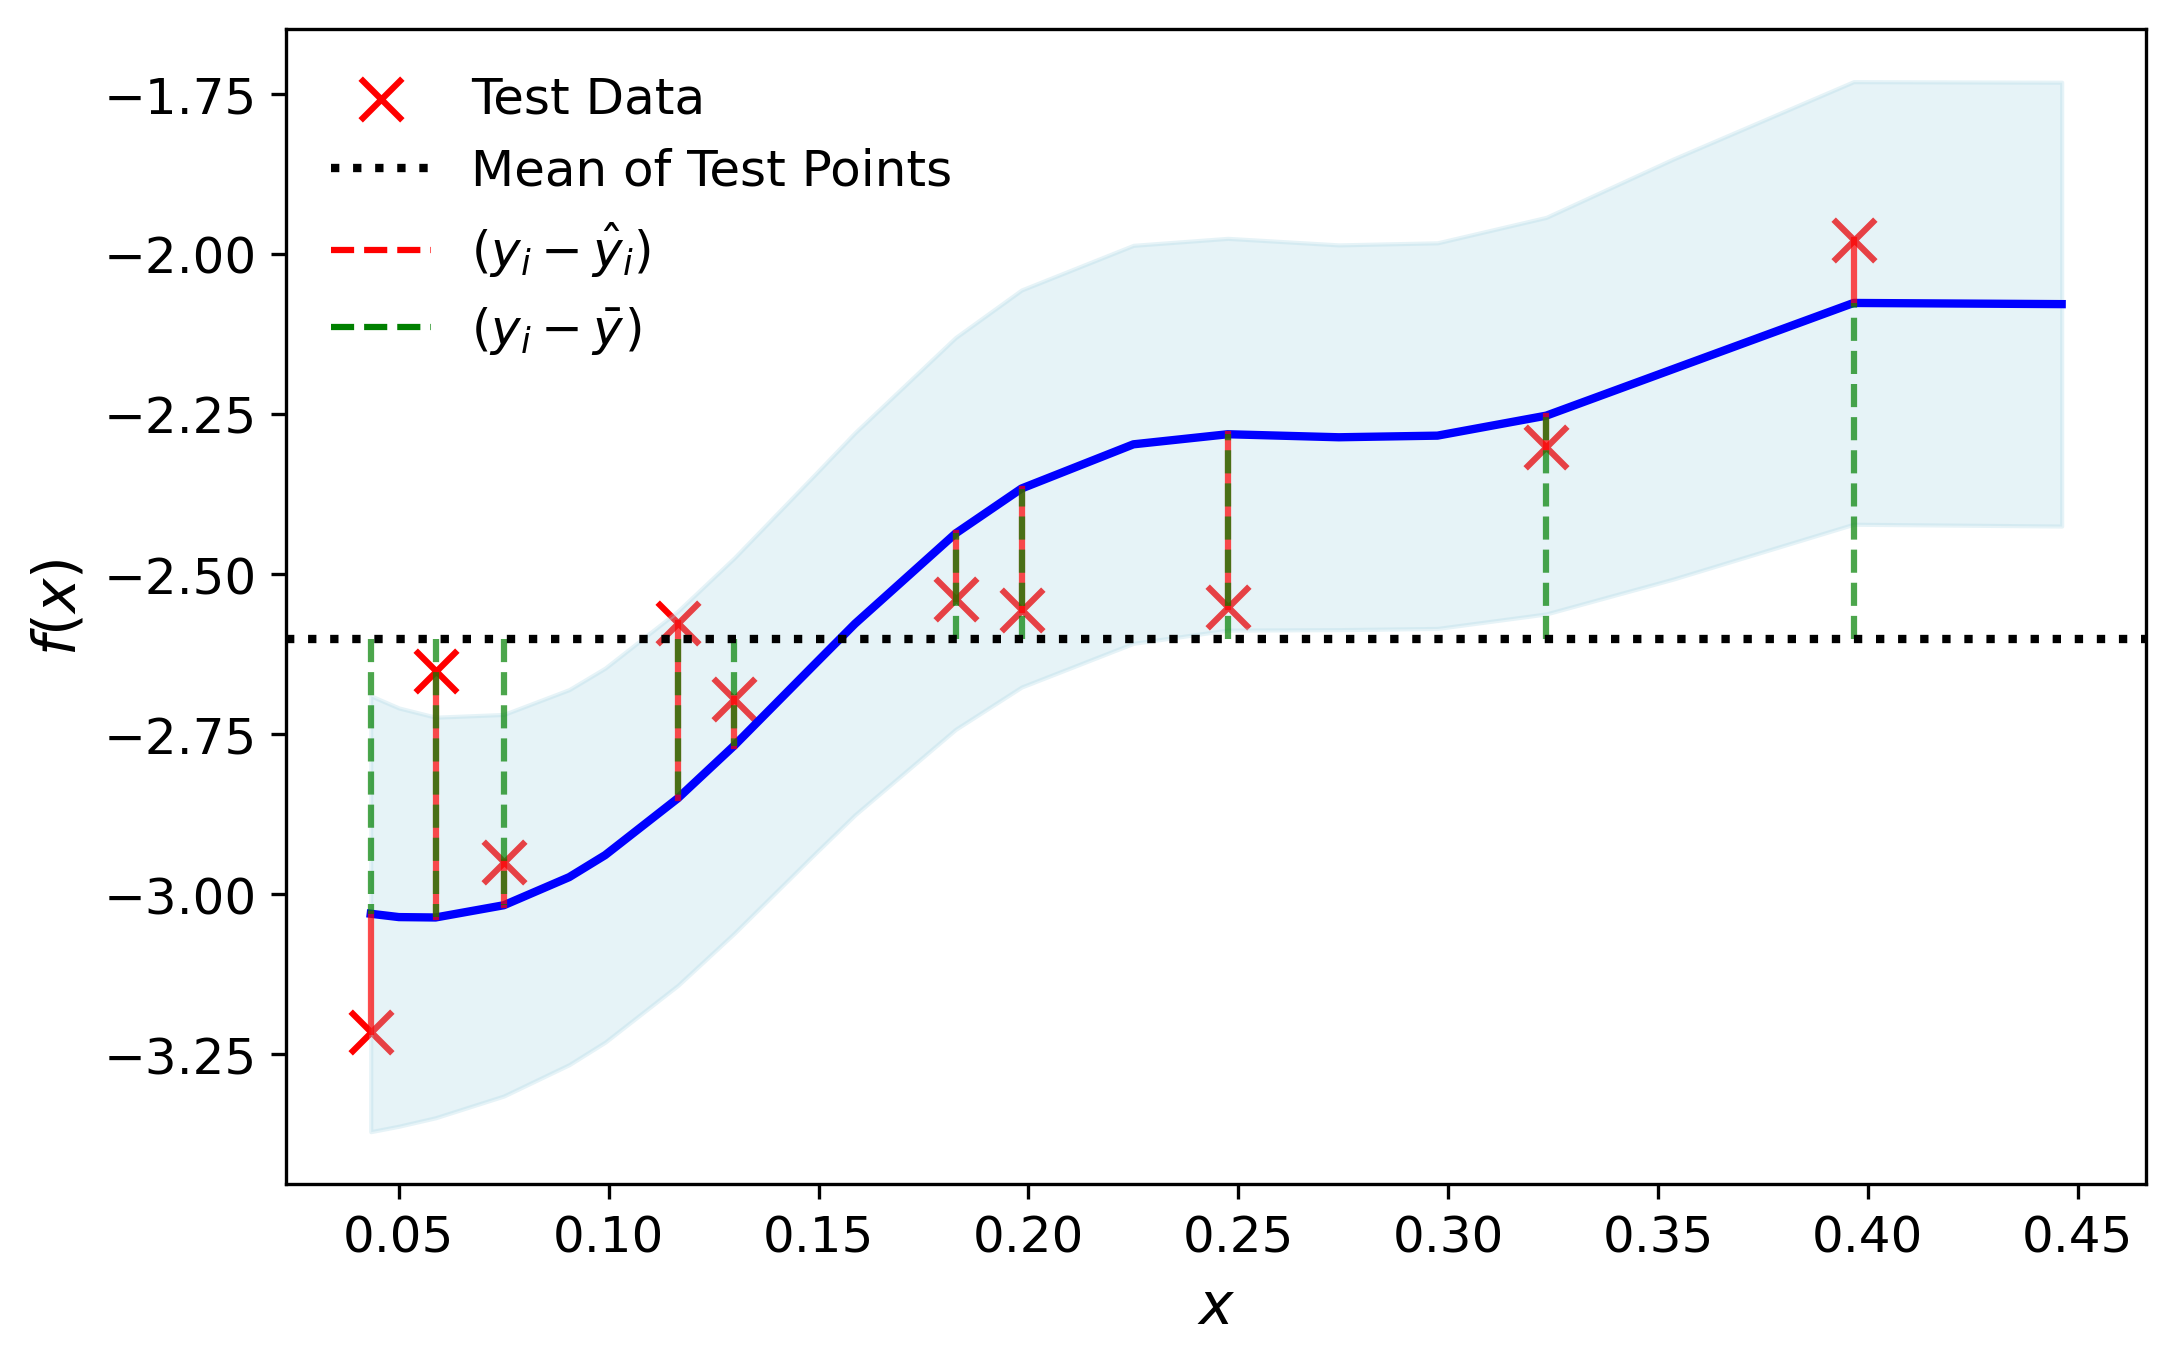
\includegraphics[width=3cm]{LatexPlots/1dplots/r2.png}} &  
        \adjustbox{valign=c}{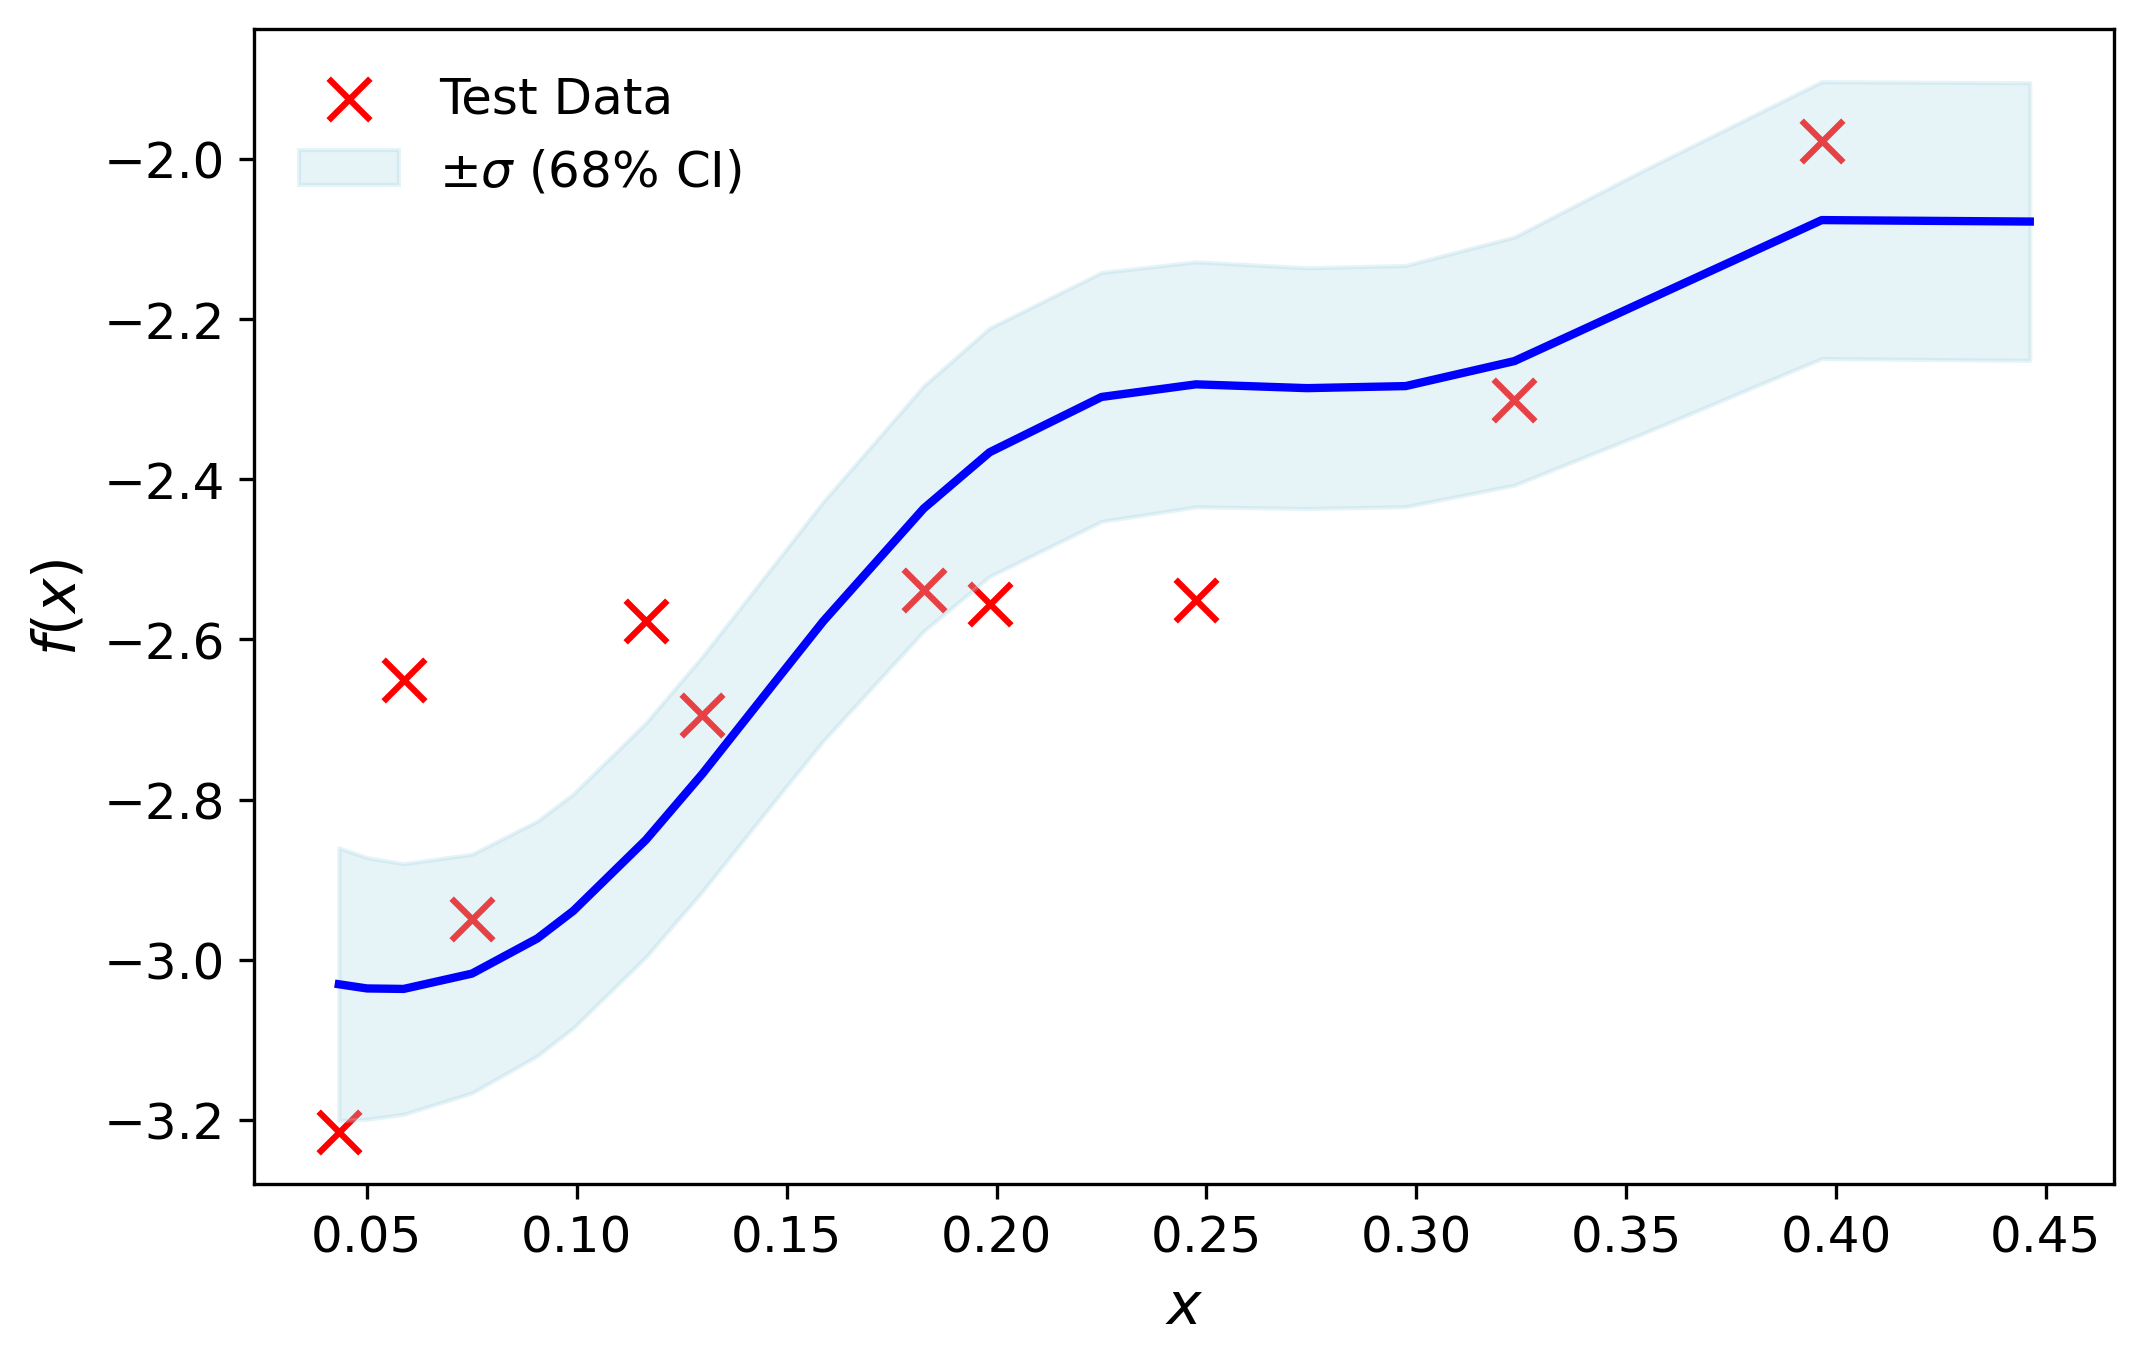
\includegraphics[width=3cm]{LatexPlots/1dplots/fom.png}} &  
        \adjustbox{valign=c}{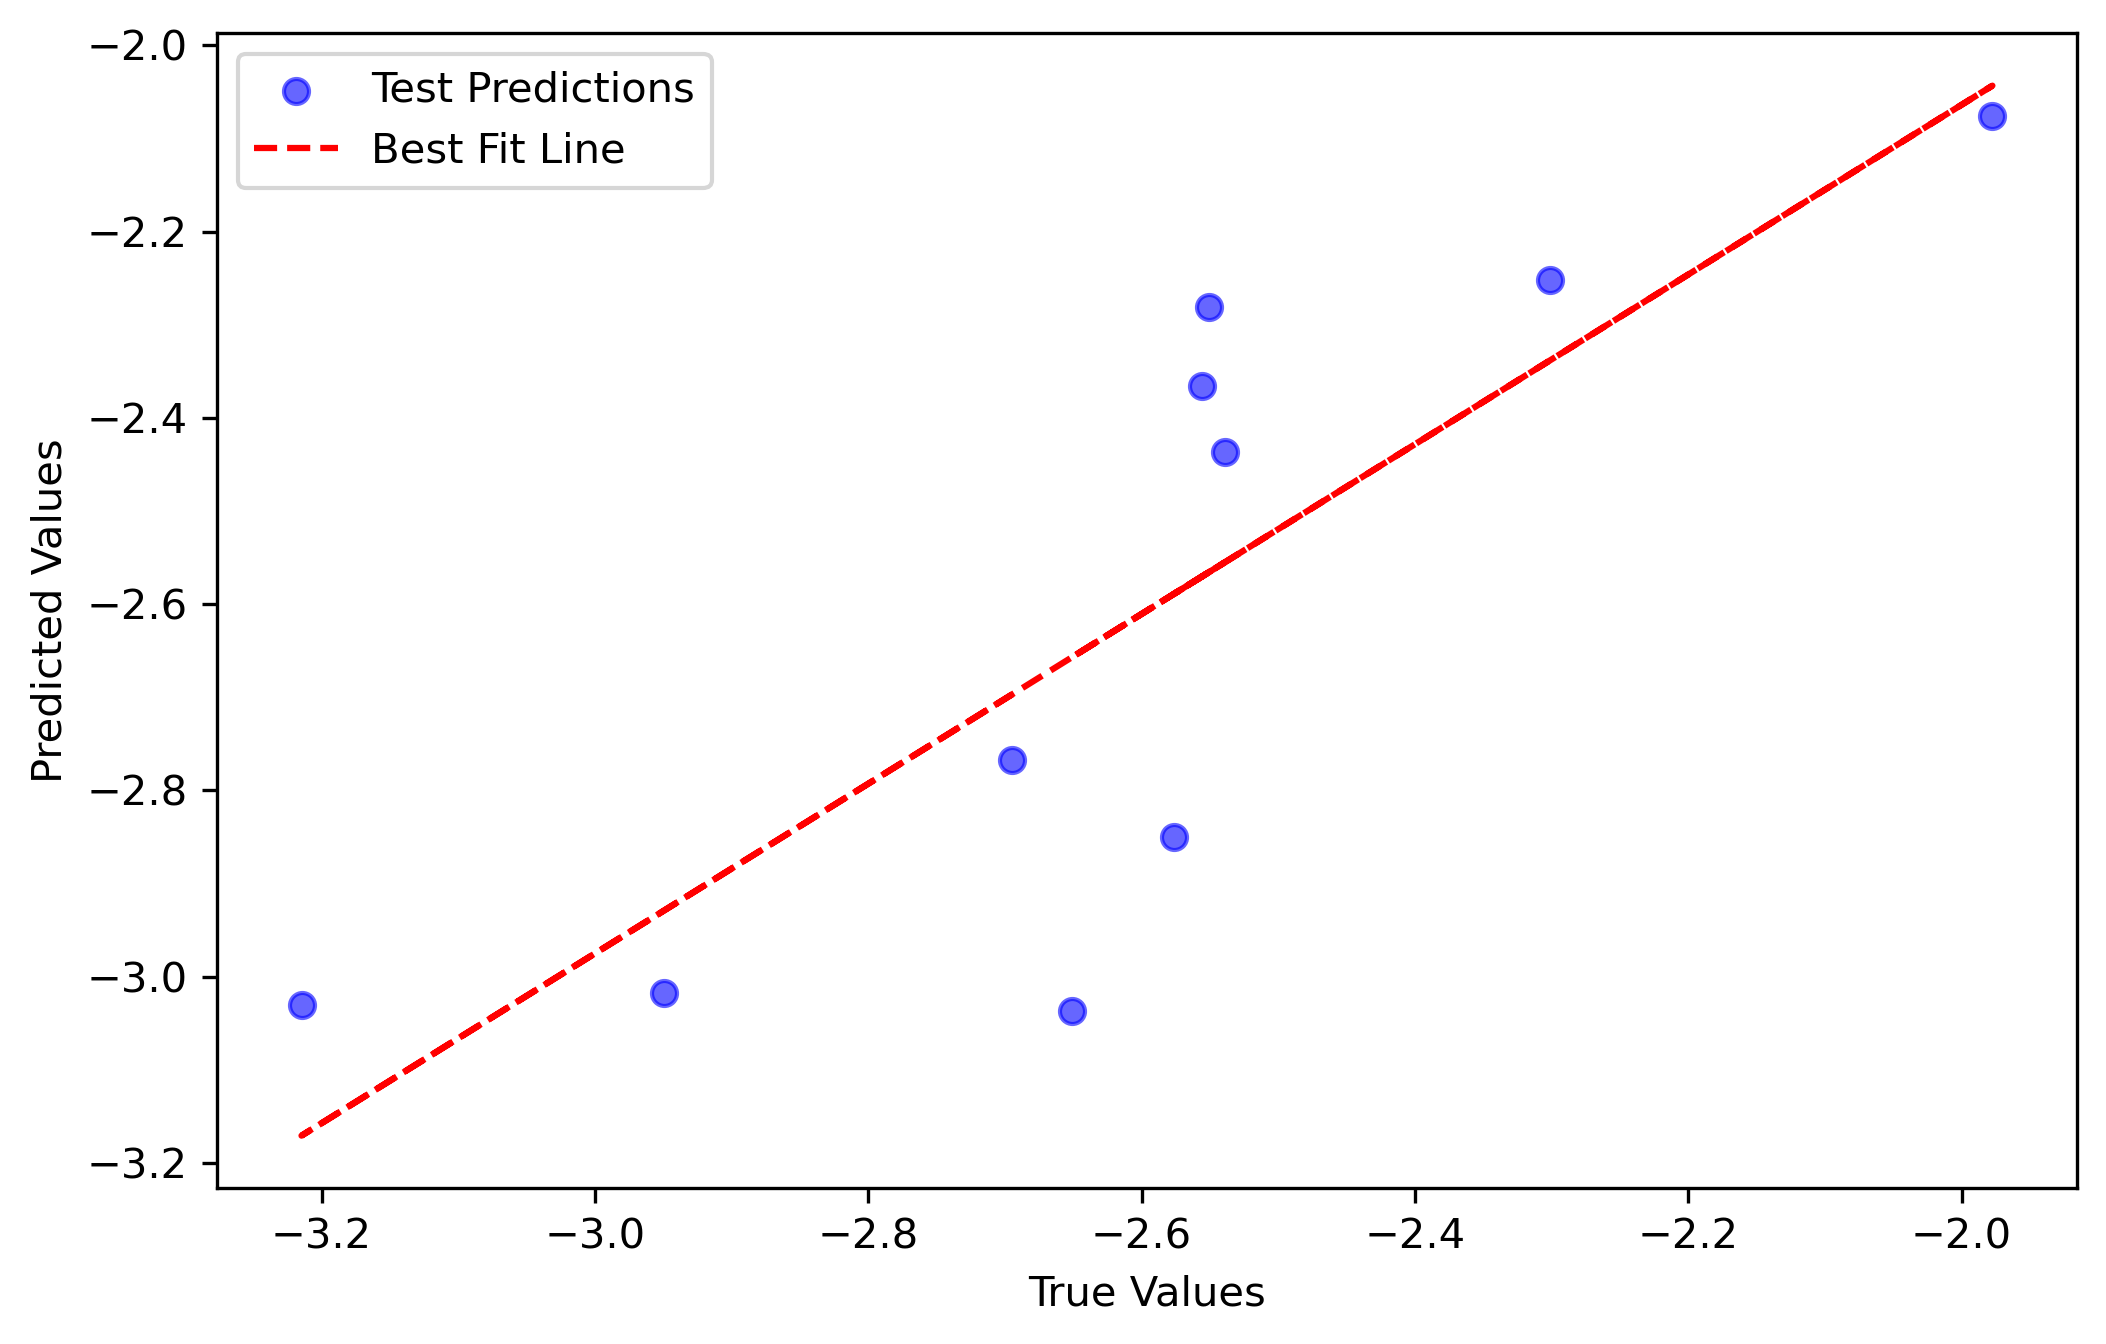
\includegraphics[width=3cm]{LatexPlots/1dplots/pearson.png}} \\  
        \hline
    \end{tabular}
    
    \caption{Comparison of different performance metrics used in evaluating models.  
    RMSE, \( R^2 \), FOM, and the Pearson Coefficient are included.  
    MAE is similar to RMSE but without squaring errors.  
    Adjusted \( R^2 \) accounts for the number of predictors and is slightly modified from \( R^2 \).
    The actual metrics for each graph are: RMSE = 0.2, \( R^2 \) = 0.6, FOM = 1.09, Pearson correlation = 0.8.}
    
    \label{tab:metrics-comparison}
\end{table}




\section{Appendix F: MCMC details}
\subsubsection*{Implementing MCMC}
\begin{figure}[H]
    \centering
    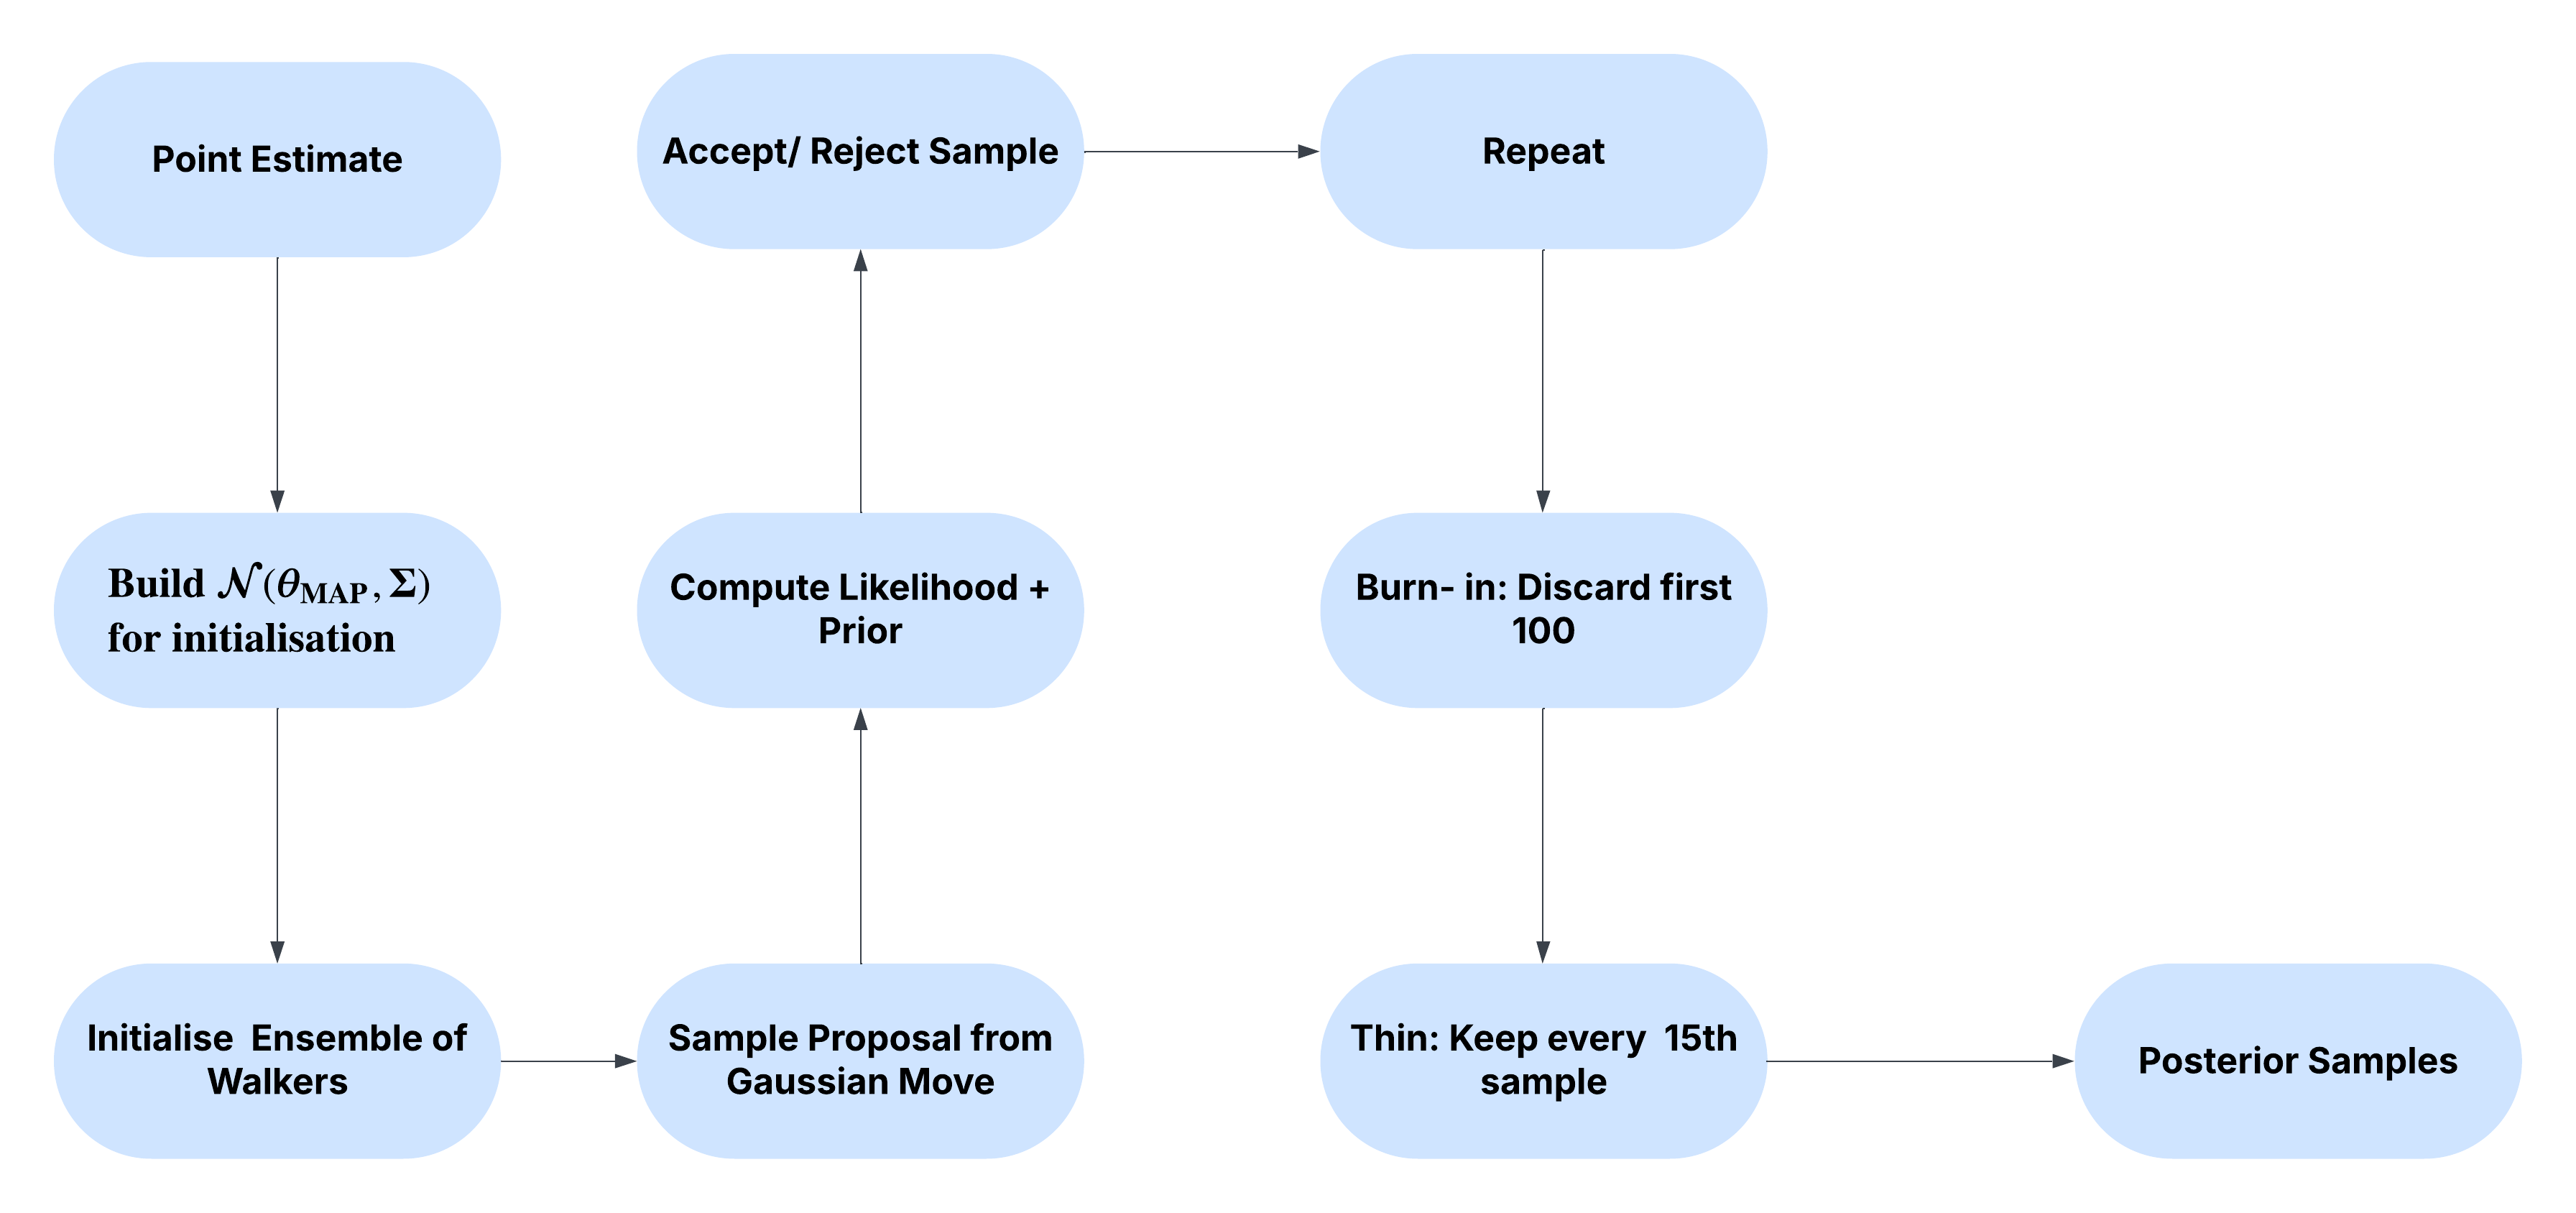
\includegraphics[width=0.8\textwidth]{LatexPlots/MCMC_Flow.png}
    \caption{Overview of the MCMC sampling procedure for Gaussian Process hyperparameter inference.
     This pipeline samples from the posterior \( p(\theta \mid \mathbf{y}, X) \) using a Metropolis-Hastings Gaussian proposal and an ensemble of walkers.}
    \label{fig:MCMC flowchart}
\end{figure}

\noindent
Before starting MCMC, we must decide which model we want to build the hyperparameter posterior for. This involves selecting one of the six kernels outlined in Section~\ref{sec: Kernels}, along with one of the three noise-modelling approaches described in Section~\ref{sec: Handlingnoise}. Once this model structure is fixed, we obtain initial point estimates for the hyperparameters by maximising the log marginal likelihood, as discussed in Section~\ref{sec: Hyper_parameters}.

\noindent
We then construct a multivariate normal distribution centred at this point estimate and sample from it to initialise each walker. From there, the walkers explore the hyperparameter space using a Gaussian proposal distribution with a specified covariance. At each step, we compute the sum of the log likelihood and log prior. The proposed sample is then accepted or rejected using the Metropolis-Hastings criterion \textcolor{red}{Could give more detail here}. This process is repeated for a fixed number of steps to generate a large set of samples.

\noindent
To ensure convergence and sample independence, we discard the first 100 samples from each walker as burn-in and apply a thinning factor of 15—retaining every 15\textsuperscript{th} sample. The resulting collection of samples forms our posterior distribution over hyperparameters, which we visualise using a kernel density estimate (KDE).


\section{Appendix G: Noise modeling using Monte Carlo Sampling}
\label{appendix:monte_carlo}

We assume the observation noise is Gaussian:
\[
\epsilon_i \sim \mathcal{N}(0, \sigma_i^2),
\]
we have the observed data \( y \) which is a noisy version of our true function values
\[
y = f + \epsilon, \quad \text{with } y \sim \mathcal{N}(f, \Sigma),
\]
where \( \Sigma = \mathrm{diag}(\sigma_1^2, \dots, \sigma_n^2) \).
Each true function value corresponds to our observed value \(\pm \epsilon\)
To account for this, we generate \( M \) noisy samples of the observations
\begin{equation}
    y^{(s)} = y + \epsilon^{(s)}, \quad \epsilon^{(s)} \sim \mathcal{N}(0, \Sigma).
\end{equation}
For each sampled dataset \( y^{(s)} \), we compute a GP posterior
\begin{equation}
    p(f_* \mid X, X_*, \theta, y^{(s)}).
\end{equation}
To obtain the final predictive distribution, we marginalize over these sampled posteriors:
\begin{equation}
    p(f_* \mid X, X_*, \theta, y) = \int p(f_* \mid X, X_*, \theta, y^{(s)}) \, p(y^{(s)} \mid y) \, dy^{(s)}.
\end{equation}
This integral is intractable so we approximate it using Monte Carlo integration where we get the average of each of our predictions on sampled datasets \(y^{(s)}\):
\begin{equation}
    p(f_* \mid X, X_*, \theta, y) \approx \frac{1}{M} \sum_{s=1}^{M} p(f_* \mid X, X_*, \theta, y^{(s)}).
\end{equation}

% %\printbibliography
% \bibliographystyle{acm}
% \bibliography{references}
\bibliography{references} 

\end{document}


